% Included from main.tex with % Included from main.tex with % Included from main.tex with % Included from main.tex with \include{sections/results}
\section{Results}
\label{sec:results}

We evaluate on four long-context benchmarks: needle retrieval, multi-document
question answering, code completion over whole repositories, and long-form
summarisation. All models are 7B-parameter decoders fine-tuned at 32k tokens
and evaluated at up to 128k.

\begin{table}[ht]
  \centering
  \caption{Accuracy and keys read per query at 128k tokens. Higher accuracy is
  better; fewer keys is cheaper. Best sparse result in bold.}
  \label{tab:results}
  \begin{tabular}{lrrrr}
    \toprule
    Method        & Needle & Multi-doc QA & Repo code & Keys read \\
    \midrule
    Dense         & 99.1   & 71.4         & 58.2      & 131{,}072 \\
    Sliding window & 41.7  & 52.9         & 44.0      & 4{,}096   \\
    BigBird       & 88.3   & 63.0         & 51.6      & 12{,}288  \\
    Routing       & 95.6   & 68.1         & 55.9      & 16{,}384  \\
    \midrule
    \textsc{Sieve} ($k=8$)  & 97.8 & 69.9 & 56.7 & 6{,}144 \\
    \textsc{Sieve} ($k=16$) & \textbf{98.9} & \textbf{71.0} & \textbf{57.8} & 11{,}264 \\
    \bottomrule
  \end{tabular}
\end{table}

Table~\ref{tab:results} summarises the main comparison. \textsc{Sieve} with
$k = 16$ is within 0.4 points of dense attention on every task while reading
$11.6\times$ fewer keys. Sliding-window attention fails at needle retrieval,
as expected, because the answer is rarely local to the question.

\begin{figure}[ht]
  \centering
  \input{figures/loss.pgf}
  \caption{Validation loss during fine-tuning. \textsc{Sieve} tracks dense
  attention closely; the shaded band is the spread over three seeds.}
  \label{fig:loss}
\end{figure}

Figure~\ref{fig:loss} shows that training with \textsc{Sieve} converges at the
same rate as dense attention, and Figure~\ref{fig:attention} shows why: the
selected blocks cover the bright regions of the dense attention map.

\begin{figure}[ht]
  \centering
  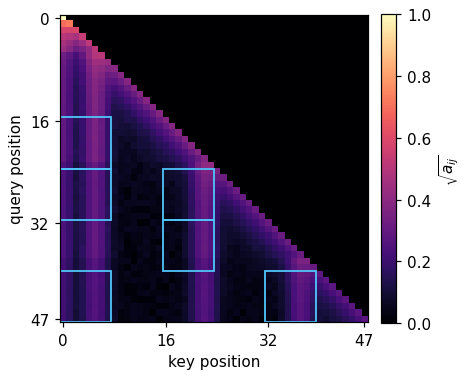
\includegraphics[width=0.8\linewidth]{figures/attention.png}
  \caption{Dense attention weights for one head of layer 18 on a 4k-token
  excerpt. Blocks selected by \textsc{Sieve} are outlined.}
  \label{fig:attention}
\end{figure}

\subsection{Ablations}

Removing the spread term $\sigma_i$ from the block score costs 2.1 points on
needle retrieval, and disabling selection reuse across layers increases
latency by 18\% with no change in accuracy. See \autoref{sec:analysis} for
why the spread term matters.

\section{Results}
\label{sec:results}

We evaluate on four long-context benchmarks: needle retrieval, multi-document
question answering, code completion over whole repositories, and long-form
summarisation. All models are 7B-parameter decoders fine-tuned at 32k tokens
and evaluated at up to 128k.

\begin{table}[ht]
  \centering
  \caption{Accuracy and keys read per query at 128k tokens. Higher accuracy is
  better; fewer keys is cheaper. Best sparse result in bold.}
  \label{tab:results}
  \begin{tabular}{lrrrr}
    \toprule
    Method        & Needle & Multi-doc QA & Repo code & Keys read \\
    \midrule
    Dense         & 99.1   & 71.4         & 58.2      & 131{,}072 \\
    Sliding window & 41.7  & 52.9         & 44.0      & 4{,}096   \\
    BigBird       & 88.3   & 63.0         & 51.6      & 12{,}288  \\
    Routing       & 95.6   & 68.1         & 55.9      & 16{,}384  \\
    \midrule
    \textsc{Sieve} ($k=8$)  & 97.8 & 69.9 & 56.7 & 6{,}144 \\
    \textsc{Sieve} ($k=16$) & \textbf{98.9} & \textbf{71.0} & \textbf{57.8} & 11{,}264 \\
    \bottomrule
  \end{tabular}
\end{table}

Table~\ref{tab:results} summarises the main comparison. \textsc{Sieve} with
$k = 16$ is within 0.4 points of dense attention on every task while reading
$11.6\times$ fewer keys. Sliding-window attention fails at needle retrieval,
as expected, because the answer is rarely local to the question.

\begin{figure}[ht]
  \centering
  %% Creator: Matplotlib, PGF backend
%%
%% To include the figure in your LaTeX document, write
%%   \input{<filename>.pgf}
%%
%% Make sure the required packages are loaded in your preamble
%%   \usepackage{pgf}
%%
%% Also ensure that all the required font packages are loaded; for instance,
%% the lmodern package is sometimes necessary when using math font.
%%   \usepackage{lmodern}
%%
%% Figures using additional raster images can only be included by \input if
%% they are in the same directory as the main LaTeX file. For loading figures
%% from other directories you can use the `import` package
%%   \usepackage{import}
%%
%% and then include the figures with
%%   \import{<path to file>}{<filename>.pgf}
%%
%% Matplotlib used the following preamble
%%   \def\mathdefault#1{#1}
%%   \everymath=\expandafter{\the\everymath\displaystyle}
%%   
%%   \ifdefined\pdftexversion\else  % non-pdftex case.
%%     \usepackage{fontspec}
%%     \setmainfont{DejaVuSerif.ttf}[Path=\detokenize{/Library/Frameworks/Python.framework/Versions/3.12/lib/python3.12/site-packages/matplotlib/mpl-data/fonts/ttf/}]
%%     \setsansfont{DejaVuSans.ttf}[Path=\detokenize{/Library/Frameworks/Python.framework/Versions/3.12/lib/python3.12/site-packages/matplotlib/mpl-data/fonts/ttf/}]
%%     \setmonofont{DejaVuSansMono.ttf}[Path=\detokenize{/Library/Frameworks/Python.framework/Versions/3.12/lib/python3.12/site-packages/matplotlib/mpl-data/fonts/ttf/}]
%%   \fi
%%   \makeatletter\@ifpackageloaded{underscore}{}{\usepackage[strings]{underscore}}\makeatother
%%
\begingroup%
\makeatletter%
\begin{pgfpicture}%
\pgfpathrectangle{\pgfpointorigin}{\pgfqpoint{4.600000in}{2.900000in}}%
\pgfusepath{use as bounding box, clip}%
\begin{pgfscope}%
\pgfsetbuttcap%
\pgfsetmiterjoin%
\definecolor{currentfill}{rgb}{1.000000,1.000000,1.000000}%
\pgfsetfillcolor{currentfill}%
\pgfsetlinewidth{0.000000pt}%
\definecolor{currentstroke}{rgb}{1.000000,1.000000,1.000000}%
\pgfsetstrokecolor{currentstroke}%
\pgfsetdash{}{0pt}%
\pgfpathmoveto{\pgfqpoint{0.000000in}{0.000000in}}%
\pgfpathlineto{\pgfqpoint{4.600000in}{0.000000in}}%
\pgfpathlineto{\pgfqpoint{4.600000in}{2.900000in}}%
\pgfpathlineto{\pgfqpoint{0.000000in}{2.900000in}}%
\pgfpathlineto{\pgfqpoint{0.000000in}{0.000000in}}%
\pgfpathclose%
\pgfusepath{fill}%
\end{pgfscope}%
\begin{pgfscope}%
\pgfsetbuttcap%
\pgfsetmiterjoin%
\definecolor{currentfill}{rgb}{1.000000,1.000000,1.000000}%
\pgfsetfillcolor{currentfill}%
\pgfsetlinewidth{0.000000pt}%
\definecolor{currentstroke}{rgb}{0.000000,0.000000,0.000000}%
\pgfsetstrokecolor{currentstroke}%
\pgfsetstrokeopacity{0.000000}%
\pgfsetdash{}{0pt}%
\pgfpathmoveto{\pgfqpoint{0.942108in}{0.582778in}}%
\pgfpathlineto{\pgfqpoint{4.450000in}{0.582778in}}%
\pgfpathlineto{\pgfqpoint{4.450000in}{2.750000in}}%
\pgfpathlineto{\pgfqpoint{0.942108in}{2.750000in}}%
\pgfpathlineto{\pgfqpoint{0.942108in}{0.582778in}}%
\pgfpathclose%
\pgfusepath{fill}%
\end{pgfscope}%
\begin{pgfscope}%
\pgfpathrectangle{\pgfqpoint{0.942108in}{0.582778in}}{\pgfqpoint{3.507892in}{2.167222in}}%
\pgfusepath{clip}%
\pgfsetbuttcap%
\pgfsetroundjoin%
\definecolor{currentfill}{rgb}{1.000000,0.584314,0.000000}%
\pgfsetfillcolor{currentfill}%
\pgfsetfillopacity{0.180000}%
\pgfsetlinewidth{0.000000pt}%
\definecolor{currentstroke}{rgb}{1.000000,0.584314,0.000000}%
\pgfsetstrokecolor{currentstroke}%
\pgfsetstrokeopacity{0.180000}%
\pgfsetdash{}{0pt}%
\pgfsys@defobject{currentmarker}{\pgfqpoint{1.101557in}{0.700885in}}{\pgfqpoint{4.290550in}{2.495498in}}{%
\pgfpathmoveto{\pgfqpoint{1.101557in}{2.495498in}}%
\pgfpathlineto{\pgfqpoint{1.101557in}{2.417550in}}%
\pgfpathlineto{\pgfqpoint{1.121488in}{2.374273in}}%
\pgfpathlineto{\pgfqpoint{1.141420in}{2.310227in}}%
\pgfpathlineto{\pgfqpoint{1.161351in}{2.287531in}}%
\pgfpathlineto{\pgfqpoint{1.181282in}{2.240011in}}%
\pgfpathlineto{\pgfqpoint{1.201213in}{2.215017in}}%
\pgfpathlineto{\pgfqpoint{1.221144in}{2.162805in}}%
\pgfpathlineto{\pgfqpoint{1.241076in}{2.119581in}}%
\pgfpathlineto{\pgfqpoint{1.261007in}{2.085505in}}%
\pgfpathlineto{\pgfqpoint{1.280938in}{2.050904in}}%
\pgfpathlineto{\pgfqpoint{1.300869in}{2.008160in}}%
\pgfpathlineto{\pgfqpoint{1.320800in}{1.976095in}}%
\pgfpathlineto{\pgfqpoint{1.340732in}{1.929877in}}%
\pgfpathlineto{\pgfqpoint{1.360663in}{1.904543in}}%
\pgfpathlineto{\pgfqpoint{1.380594in}{1.879047in}}%
\pgfpathlineto{\pgfqpoint{1.400525in}{1.856081in}}%
\pgfpathlineto{\pgfqpoint{1.420457in}{1.812893in}}%
\pgfpathlineto{\pgfqpoint{1.440388in}{1.777388in}}%
\pgfpathlineto{\pgfqpoint{1.460319in}{1.754407in}}%
\pgfpathlineto{\pgfqpoint{1.480250in}{1.722701in}}%
\pgfpathlineto{\pgfqpoint{1.500181in}{1.698938in}}%
\pgfpathlineto{\pgfqpoint{1.520113in}{1.664865in}}%
\pgfpathlineto{\pgfqpoint{1.540044in}{1.625673in}}%
\pgfpathlineto{\pgfqpoint{1.559975in}{1.601581in}}%
\pgfpathlineto{\pgfqpoint{1.579906in}{1.573959in}}%
\pgfpathlineto{\pgfqpoint{1.599837in}{1.548897in}}%
\pgfpathlineto{\pgfqpoint{1.619769in}{1.522375in}}%
\pgfpathlineto{\pgfqpoint{1.639700in}{1.488027in}}%
\pgfpathlineto{\pgfqpoint{1.659631in}{1.450840in}}%
\pgfpathlineto{\pgfqpoint{1.679562in}{1.441056in}}%
\pgfpathlineto{\pgfqpoint{1.699493in}{1.404633in}}%
\pgfpathlineto{\pgfqpoint{1.719425in}{1.402809in}}%
\pgfpathlineto{\pgfqpoint{1.739356in}{1.380364in}}%
\pgfpathlineto{\pgfqpoint{1.759287in}{1.342313in}}%
\pgfpathlineto{\pgfqpoint{1.779218in}{1.345331in}}%
\pgfpathlineto{\pgfqpoint{1.799149in}{1.327086in}}%
\pgfpathlineto{\pgfqpoint{1.819081in}{1.299820in}}%
\pgfpathlineto{\pgfqpoint{1.839012in}{1.296794in}}%
\pgfpathlineto{\pgfqpoint{1.858943in}{1.280513in}}%
\pgfpathlineto{\pgfqpoint{1.878874in}{1.231137in}}%
\pgfpathlineto{\pgfqpoint{1.898805in}{1.236844in}}%
\pgfpathlineto{\pgfqpoint{1.918737in}{1.213867in}}%
\pgfpathlineto{\pgfqpoint{1.938668in}{1.197274in}}%
\pgfpathlineto{\pgfqpoint{1.958599in}{1.186760in}}%
\pgfpathlineto{\pgfqpoint{1.978530in}{1.154095in}}%
\pgfpathlineto{\pgfqpoint{1.998462in}{1.140456in}}%
\pgfpathlineto{\pgfqpoint{2.018393in}{1.123469in}}%
\pgfpathlineto{\pgfqpoint{2.038324in}{1.110151in}}%
\pgfpathlineto{\pgfqpoint{2.058255in}{1.103458in}}%
\pgfpathlineto{\pgfqpoint{2.078186in}{1.075874in}}%
\pgfpathlineto{\pgfqpoint{2.098118in}{1.067387in}}%
\pgfpathlineto{\pgfqpoint{2.118049in}{1.072241in}}%
\pgfpathlineto{\pgfqpoint{2.137980in}{1.053360in}}%
\pgfpathlineto{\pgfqpoint{2.157911in}{1.046571in}}%
\pgfpathlineto{\pgfqpoint{2.177842in}{1.011003in}}%
\pgfpathlineto{\pgfqpoint{2.197774in}{1.011974in}}%
\pgfpathlineto{\pgfqpoint{2.217705in}{1.003878in}}%
\pgfpathlineto{\pgfqpoint{2.237636in}{0.999971in}}%
\pgfpathlineto{\pgfqpoint{2.257567in}{0.983480in}}%
\pgfpathlineto{\pgfqpoint{2.277498in}{0.990178in}}%
\pgfpathlineto{\pgfqpoint{2.297430in}{0.970365in}}%
\pgfpathlineto{\pgfqpoint{2.317361in}{0.962247in}}%
\pgfpathlineto{\pgfqpoint{2.337292in}{0.953582in}}%
\pgfpathlineto{\pgfqpoint{2.357223in}{0.952656in}}%
\pgfpathlineto{\pgfqpoint{2.377154in}{0.931985in}}%
\pgfpathlineto{\pgfqpoint{2.397086in}{0.941206in}}%
\pgfpathlineto{\pgfqpoint{2.417017in}{0.926623in}}%
\pgfpathlineto{\pgfqpoint{2.436948in}{0.916085in}}%
\pgfpathlineto{\pgfqpoint{2.456879in}{0.907859in}}%
\pgfpathlineto{\pgfqpoint{2.476810in}{0.906163in}}%
\pgfpathlineto{\pgfqpoint{2.496742in}{0.904850in}}%
\pgfpathlineto{\pgfqpoint{2.516673in}{0.897768in}}%
\pgfpathlineto{\pgfqpoint{2.536604in}{0.885615in}}%
\pgfpathlineto{\pgfqpoint{2.556535in}{0.885001in}}%
\pgfpathlineto{\pgfqpoint{2.576467in}{0.871282in}}%
\pgfpathlineto{\pgfqpoint{2.596398in}{0.877727in}}%
\pgfpathlineto{\pgfqpoint{2.616329in}{0.858941in}}%
\pgfpathlineto{\pgfqpoint{2.636260in}{0.832128in}}%
\pgfpathlineto{\pgfqpoint{2.656191in}{0.863177in}}%
\pgfpathlineto{\pgfqpoint{2.676123in}{0.845518in}}%
\pgfpathlineto{\pgfqpoint{2.696054in}{0.827485in}}%
\pgfpathlineto{\pgfqpoint{2.715985in}{0.833274in}}%
\pgfpathlineto{\pgfqpoint{2.735916in}{0.821827in}}%
\pgfpathlineto{\pgfqpoint{2.755847in}{0.848677in}}%
\pgfpathlineto{\pgfqpoint{2.775779in}{0.828111in}}%
\pgfpathlineto{\pgfqpoint{2.795710in}{0.802798in}}%
\pgfpathlineto{\pgfqpoint{2.815641in}{0.821040in}}%
\pgfpathlineto{\pgfqpoint{2.835572in}{0.807719in}}%
\pgfpathlineto{\pgfqpoint{2.855503in}{0.828004in}}%
\pgfpathlineto{\pgfqpoint{2.875435in}{0.794247in}}%
\pgfpathlineto{\pgfqpoint{2.895366in}{0.778763in}}%
\pgfpathlineto{\pgfqpoint{2.915297in}{0.799455in}}%
\pgfpathlineto{\pgfqpoint{2.935228in}{0.792266in}}%
\pgfpathlineto{\pgfqpoint{2.955159in}{0.788714in}}%
\pgfpathlineto{\pgfqpoint{2.975091in}{0.768414in}}%
\pgfpathlineto{\pgfqpoint{2.995022in}{0.791818in}}%
\pgfpathlineto{\pgfqpoint{3.014953in}{0.801711in}}%
\pgfpathlineto{\pgfqpoint{3.034884in}{0.763259in}}%
\pgfpathlineto{\pgfqpoint{3.054815in}{0.791773in}}%
\pgfpathlineto{\pgfqpoint{3.074747in}{0.772132in}}%
\pgfpathlineto{\pgfqpoint{3.094678in}{0.798798in}}%
\pgfpathlineto{\pgfqpoint{3.114609in}{0.777778in}}%
\pgfpathlineto{\pgfqpoint{3.134540in}{0.769560in}}%
\pgfpathlineto{\pgfqpoint{3.154472in}{0.780285in}}%
\pgfpathlineto{\pgfqpoint{3.174403in}{0.772687in}}%
\pgfpathlineto{\pgfqpoint{3.194334in}{0.759906in}}%
\pgfpathlineto{\pgfqpoint{3.214265in}{0.770844in}}%
\pgfpathlineto{\pgfqpoint{3.234196in}{0.757275in}}%
\pgfpathlineto{\pgfqpoint{3.254128in}{0.743228in}}%
\pgfpathlineto{\pgfqpoint{3.274059in}{0.778522in}}%
\pgfpathlineto{\pgfqpoint{3.293990in}{0.754145in}}%
\pgfpathlineto{\pgfqpoint{3.313921in}{0.750206in}}%
\pgfpathlineto{\pgfqpoint{3.333852in}{0.757868in}}%
\pgfpathlineto{\pgfqpoint{3.353784in}{0.738404in}}%
\pgfpathlineto{\pgfqpoint{3.373715in}{0.739117in}}%
\pgfpathlineto{\pgfqpoint{3.393646in}{0.746003in}}%
\pgfpathlineto{\pgfqpoint{3.413577in}{0.744622in}}%
\pgfpathlineto{\pgfqpoint{3.433508in}{0.749027in}}%
\pgfpathlineto{\pgfqpoint{3.453440in}{0.757690in}}%
\pgfpathlineto{\pgfqpoint{3.473371in}{0.741741in}}%
\pgfpathlineto{\pgfqpoint{3.493302in}{0.749682in}}%
\pgfpathlineto{\pgfqpoint{3.513233in}{0.749669in}}%
\pgfpathlineto{\pgfqpoint{3.533164in}{0.733162in}}%
\pgfpathlineto{\pgfqpoint{3.553096in}{0.744330in}}%
\pgfpathlineto{\pgfqpoint{3.573027in}{0.732720in}}%
\pgfpathlineto{\pgfqpoint{3.592958in}{0.750149in}}%
\pgfpathlineto{\pgfqpoint{3.612889in}{0.743789in}}%
\pgfpathlineto{\pgfqpoint{3.632821in}{0.739025in}}%
\pgfpathlineto{\pgfqpoint{3.652752in}{0.726028in}}%
\pgfpathlineto{\pgfqpoint{3.672683in}{0.738420in}}%
\pgfpathlineto{\pgfqpoint{3.692614in}{0.729817in}}%
\pgfpathlineto{\pgfqpoint{3.712545in}{0.742266in}}%
\pgfpathlineto{\pgfqpoint{3.732477in}{0.734287in}}%
\pgfpathlineto{\pgfqpoint{3.752408in}{0.727536in}}%
\pgfpathlineto{\pgfqpoint{3.772339in}{0.742233in}}%
\pgfpathlineto{\pgfqpoint{3.792270in}{0.739840in}}%
\pgfpathlineto{\pgfqpoint{3.812201in}{0.727793in}}%
\pgfpathlineto{\pgfqpoint{3.832133in}{0.742508in}}%
\pgfpathlineto{\pgfqpoint{3.852064in}{0.729337in}}%
\pgfpathlineto{\pgfqpoint{3.871995in}{0.728757in}}%
\pgfpathlineto{\pgfqpoint{3.891926in}{0.732009in}}%
\pgfpathlineto{\pgfqpoint{3.911857in}{0.724041in}}%
\pgfpathlineto{\pgfqpoint{3.931789in}{0.726280in}}%
\pgfpathlineto{\pgfqpoint{3.951720in}{0.728259in}}%
\pgfpathlineto{\pgfqpoint{3.971651in}{0.742106in}}%
\pgfpathlineto{\pgfqpoint{3.991582in}{0.741407in}}%
\pgfpathlineto{\pgfqpoint{4.011513in}{0.726273in}}%
\pgfpathlineto{\pgfqpoint{4.031445in}{0.741487in}}%
\pgfpathlineto{\pgfqpoint{4.051376in}{0.727374in}}%
\pgfpathlineto{\pgfqpoint{4.071307in}{0.730549in}}%
\pgfpathlineto{\pgfqpoint{4.091238in}{0.734355in}}%
\pgfpathlineto{\pgfqpoint{4.111169in}{0.729167in}}%
\pgfpathlineto{\pgfqpoint{4.131101in}{0.746147in}}%
\pgfpathlineto{\pgfqpoint{4.151032in}{0.728169in}}%
\pgfpathlineto{\pgfqpoint{4.170963in}{0.716167in}}%
\pgfpathlineto{\pgfqpoint{4.190894in}{0.736178in}}%
\pgfpathlineto{\pgfqpoint{4.210826in}{0.722074in}}%
\pgfpathlineto{\pgfqpoint{4.230757in}{0.722710in}}%
\pgfpathlineto{\pgfqpoint{4.250688in}{0.700885in}}%
\pgfpathlineto{\pgfqpoint{4.270619in}{0.732643in}}%
\pgfpathlineto{\pgfqpoint{4.290550in}{0.730954in}}%
\pgfpathlineto{\pgfqpoint{4.290550in}{0.799688in}}%
\pgfpathlineto{\pgfqpoint{4.290550in}{0.799688in}}%
\pgfpathlineto{\pgfqpoint{4.270619in}{0.801403in}}%
\pgfpathlineto{\pgfqpoint{4.250688in}{0.770748in}}%
\pgfpathlineto{\pgfqpoint{4.230757in}{0.791953in}}%
\pgfpathlineto{\pgfqpoint{4.210826in}{0.791423in}}%
\pgfpathlineto{\pgfqpoint{4.190894in}{0.805161in}}%
\pgfpathlineto{\pgfqpoint{4.170963in}{0.785882in}}%
\pgfpathlineto{\pgfqpoint{4.151032in}{0.797588in}}%
\pgfpathlineto{\pgfqpoint{4.131101in}{0.815081in}}%
\pgfpathlineto{\pgfqpoint{4.111169in}{0.798741in}}%
\pgfpathlineto{\pgfqpoint{4.091238in}{0.803858in}}%
\pgfpathlineto{\pgfqpoint{4.071307in}{0.800274in}}%
\pgfpathlineto{\pgfqpoint{4.051376in}{0.797302in}}%
\pgfpathlineto{\pgfqpoint{4.031445in}{0.811061in}}%
\pgfpathlineto{\pgfqpoint{4.011513in}{0.796444in}}%
\pgfpathlineto{\pgfqpoint{3.991582in}{0.811194in}}%
\pgfpathlineto{\pgfqpoint{3.971651in}{0.811979in}}%
\pgfpathlineto{\pgfqpoint{3.951720in}{0.798694in}}%
\pgfpathlineto{\pgfqpoint{3.931789in}{0.796894in}}%
\pgfpathlineto{\pgfqpoint{3.911857in}{0.794844in}}%
\pgfpathlineto{\pgfqpoint{3.891926in}{0.802669in}}%
\pgfpathlineto{\pgfqpoint{3.871995in}{0.799645in}}%
\pgfpathlineto{\pgfqpoint{3.852064in}{0.800329in}}%
\pgfpathlineto{\pgfqpoint{3.832133in}{0.813194in}}%
\pgfpathlineto{\pgfqpoint{3.812201in}{0.799092in}}%
\pgfpathlineto{\pgfqpoint{3.792270in}{0.810874in}}%
\pgfpathlineto{\pgfqpoint{3.772339in}{0.813321in}}%
\pgfpathlineto{\pgfqpoint{3.752408in}{0.799247in}}%
\pgfpathlineto{\pgfqpoint{3.732477in}{0.805914in}}%
\pgfpathlineto{\pgfqpoint{3.712545in}{0.813771in}}%
\pgfpathlineto{\pgfqpoint{3.692614in}{0.801882in}}%
\pgfpathlineto{\pgfqpoint{3.672683in}{0.810346in}}%
\pgfpathlineto{\pgfqpoint{3.652752in}{0.798521in}}%
\pgfpathlineto{\pgfqpoint{3.632821in}{0.811238in}}%
\pgfpathlineto{\pgfqpoint{3.612889in}{0.816000in}}%
\pgfpathlineto{\pgfqpoint{3.592958in}{0.822308in}}%
\pgfpathlineto{\pgfqpoint{3.573027in}{0.805630in}}%
\pgfpathlineto{\pgfqpoint{3.553096in}{0.817016in}}%
\pgfpathlineto{\pgfqpoint{3.533164in}{0.806398in}}%
\pgfpathlineto{\pgfqpoint{3.513233in}{0.822521in}}%
\pgfpathlineto{\pgfqpoint{3.493302in}{0.822712in}}%
\pgfpathlineto{\pgfqpoint{3.473371in}{0.815222in}}%
\pgfpathlineto{\pgfqpoint{3.453440in}{0.830816in}}%
\pgfpathlineto{\pgfqpoint{3.433508in}{0.822636in}}%
\pgfpathlineto{\pgfqpoint{3.413577in}{0.818575in}}%
\pgfpathlineto{\pgfqpoint{3.393646in}{0.820107in}}%
\pgfpathlineto{\pgfqpoint{3.373715in}{0.813661in}}%
\pgfpathlineto{\pgfqpoint{3.353784in}{0.813179in}}%
\pgfpathlineto{\pgfqpoint{3.333852in}{0.832181in}}%
\pgfpathlineto{\pgfqpoint{3.313921in}{0.824999in}}%
\pgfpathlineto{\pgfqpoint{3.293990in}{0.829020in}}%
\pgfpathlineto{\pgfqpoint{3.274059in}{0.852777in}}%
\pgfpathlineto{\pgfqpoint{3.254128in}{0.818936in}}%
\pgfpathlineto{\pgfqpoint{3.234196in}{0.832724in}}%
\pgfpathlineto{\pgfqpoint{3.214265in}{0.846057in}}%
\pgfpathlineto{\pgfqpoint{3.194334in}{0.835742in}}%
\pgfpathlineto{\pgfqpoint{3.174403in}{0.848322in}}%
\pgfpathlineto{\pgfqpoint{3.154472in}{0.855904in}}%
\pgfpathlineto{\pgfqpoint{3.134540in}{0.845812in}}%
\pgfpathlineto{\pgfqpoint{3.114609in}{0.854001in}}%
\pgfpathlineto{\pgfqpoint{3.094678in}{0.874546in}}%
\pgfpathlineto{\pgfqpoint{3.074747in}{0.849094in}}%
\pgfpathlineto{\pgfqpoint{3.054815in}{0.868314in}}%
\pgfpathlineto{\pgfqpoint{3.034884in}{0.841102in}}%
\pgfpathlineto{\pgfqpoint{3.014953in}{0.878467in}}%
\pgfpathlineto{\pgfqpoint{2.995022in}{0.869220in}}%
\pgfpathlineto{\pgfqpoint{2.975091in}{0.846961in}}%
\pgfpathlineto{\pgfqpoint{2.955159in}{0.866832in}}%
\pgfpathlineto{\pgfqpoint{2.935228in}{0.870569in}}%
\pgfpathlineto{\pgfqpoint{2.915297in}{0.877815in}}%
\pgfpathlineto{\pgfqpoint{2.895366in}{0.858204in}}%
\pgfpathlineto{\pgfqpoint{2.875435in}{0.873453in}}%
\pgfpathlineto{\pgfqpoint{2.855503in}{0.906316in}}%
\pgfpathlineto{\pgfqpoint{2.835572in}{0.887113in}}%
\pgfpathlineto{\pgfqpoint{2.815641in}{0.900295in}}%
\pgfpathlineto{\pgfqpoint{2.795710in}{0.883084in}}%
\pgfpathlineto{\pgfqpoint{2.775779in}{0.907824in}}%
\pgfpathlineto{\pgfqpoint{2.755847in}{0.928001in}}%
\pgfpathlineto{\pgfqpoint{2.735916in}{0.902521in}}%
\pgfpathlineto{\pgfqpoint{2.715985in}{0.913927in}}%
\pgfpathlineto{\pgfqpoint{2.696054in}{0.908748in}}%
\pgfpathlineto{\pgfqpoint{2.676123in}{0.926505in}}%
\pgfpathlineto{\pgfqpoint{2.656191in}{0.943908in}}%
\pgfpathlineto{\pgfqpoint{2.636260in}{0.914444in}}%
\pgfpathlineto{\pgfqpoint{2.616329in}{0.940665in}}%
\pgfpathlineto{\pgfqpoint{2.596398in}{0.959170in}}%
\pgfpathlineto{\pgfqpoint{2.576467in}{0.953405in}}%
\pgfpathlineto{\pgfqpoint{2.556535in}{0.967048in}}%
\pgfpathlineto{\pgfqpoint{2.536604in}{0.968090in}}%
\pgfpathlineto{\pgfqpoint{2.516673in}{0.980241in}}%
\pgfpathlineto{\pgfqpoint{2.496742in}{0.987521in}}%
\pgfpathlineto{\pgfqpoint{2.476810in}{0.989259in}}%
\pgfpathlineto{\pgfqpoint{2.456879in}{0.991377in}}%
\pgfpathlineto{\pgfqpoint{2.436948in}{0.999779in}}%
\pgfpathlineto{\pgfqpoint{2.417017in}{1.010414in}}%
\pgfpathlineto{\pgfqpoint{2.397086in}{1.024943in}}%
\pgfpathlineto{\pgfqpoint{2.377154in}{1.016602in}}%
\pgfpathlineto{\pgfqpoint{2.357223in}{1.036996in}}%
\pgfpathlineto{\pgfqpoint{2.337292in}{1.038425in}}%
\pgfpathlineto{\pgfqpoint{2.317361in}{1.047298in}}%
\pgfpathlineto{\pgfqpoint{2.297430in}{1.055655in}}%
\pgfpathlineto{\pgfqpoint{2.277498in}{1.075254in}}%
\pgfpathlineto{\pgfqpoint{2.257567in}{1.069397in}}%
\pgfpathlineto{\pgfqpoint{2.237636in}{1.085821in}}%
\pgfpathlineto{\pgfqpoint{2.217705in}{1.090169in}}%
\pgfpathlineto{\pgfqpoint{2.197774in}{1.098549in}}%
\pgfpathlineto{\pgfqpoint{2.177842in}{1.098235in}}%
\pgfpathlineto{\pgfqpoint{2.157911in}{1.133003in}}%
\pgfpathlineto{\pgfqpoint{2.137980in}{1.140154in}}%
\pgfpathlineto{\pgfqpoint{2.118049in}{1.158921in}}%
\pgfpathlineto{\pgfqpoint{2.098118in}{1.154917in}}%
\pgfpathlineto{\pgfqpoint{2.078186in}{1.163727in}}%
\pgfpathlineto{\pgfqpoint{2.058255in}{1.190870in}}%
\pgfpathlineto{\pgfqpoint{2.038324in}{1.197977in}}%
\pgfpathlineto{\pgfqpoint{2.018393in}{1.211449in}}%
\pgfpathlineto{\pgfqpoint{1.998462in}{1.228450in}}%
\pgfpathlineto{\pgfqpoint{1.978530in}{1.242249in}}%
\pgfpathlineto{\pgfqpoint{1.958599in}{1.274310in}}%
\pgfpathlineto{\pgfqpoint{1.938668in}{1.285127in}}%
\pgfpathlineto{\pgfqpoint{1.918737in}{1.301787in}}%
\pgfpathlineto{\pgfqpoint{1.898805in}{1.324581in}}%
\pgfpathlineto{\pgfqpoint{1.878874in}{1.319867in}}%
\pgfpathlineto{\pgfqpoint{1.858943in}{1.368003in}}%
\pgfpathlineto{\pgfqpoint{1.839012in}{1.384399in}}%
\pgfpathlineto{\pgfqpoint{1.819081in}{1.388088in}}%
\pgfpathlineto{\pgfqpoint{1.799149in}{1.415041in}}%
\pgfpathlineto{\pgfqpoint{1.779218in}{1.433350in}}%
\pgfpathlineto{\pgfqpoint{1.759287in}{1.431274in}}%
\pgfpathlineto{\pgfqpoint{1.739356in}{1.468597in}}%
\pgfpathlineto{\pgfqpoint{1.719425in}{1.490963in}}%
\pgfpathlineto{\pgfqpoint{1.699493in}{1.493559in}}%
\pgfpathlineto{\pgfqpoint{1.679562in}{1.529349in}}%
\pgfpathlineto{\pgfqpoint{1.659631in}{1.539599in}}%
\pgfpathlineto{\pgfqpoint{1.639700in}{1.576142in}}%
\pgfpathlineto{\pgfqpoint{1.619769in}{1.609975in}}%
\pgfpathlineto{\pgfqpoint{1.599837in}{1.636309in}}%
\pgfpathlineto{\pgfqpoint{1.579906in}{1.661251in}}%
\pgfpathlineto{\pgfqpoint{1.559975in}{1.688660in}}%
\pgfpathlineto{\pgfqpoint{1.540044in}{1.712691in}}%
\pgfpathlineto{\pgfqpoint{1.520113in}{1.751226in}}%
\pgfpathlineto{\pgfqpoint{1.500181in}{1.784859in}}%
\pgfpathlineto{\pgfqpoint{1.480250in}{1.808602in}}%
\pgfpathlineto{\pgfqpoint{1.460319in}{1.839982in}}%
\pgfpathlineto{\pgfqpoint{1.440388in}{1.862992in}}%
\pgfpathlineto{\pgfqpoint{1.420457in}{1.898040in}}%
\pgfpathlineto{\pgfqpoint{1.400525in}{1.940483in}}%
\pgfpathlineto{\pgfqpoint{1.380594in}{1.963505in}}%
\pgfpathlineto{\pgfqpoint{1.360663in}{1.988967in}}%
\pgfpathlineto{\pgfqpoint{1.340732in}{2.014282in}}%
\pgfpathlineto{\pgfqpoint{1.320800in}{2.059679in}}%
\pgfpathlineto{\pgfqpoint{1.300869in}{2.091484in}}%
\pgfpathlineto{\pgfqpoint{1.280938in}{2.133567in}}%
\pgfpathlineto{\pgfqpoint{1.261007in}{2.167830in}}%
\pgfpathlineto{\pgfqpoint{1.241076in}{2.201598in}}%
\pgfpathlineto{\pgfqpoint{1.221144in}{2.244179in}}%
\pgfpathlineto{\pgfqpoint{1.201213in}{2.295425in}}%
\pgfpathlineto{\pgfqpoint{1.181282in}{2.320481in}}%
\pgfpathlineto{\pgfqpoint{1.161351in}{2.367236in}}%
\pgfpathlineto{\pgfqpoint{1.141420in}{2.390093in}}%
\pgfpathlineto{\pgfqpoint{1.121488in}{2.452793in}}%
\pgfpathlineto{\pgfqpoint{1.101557in}{2.495498in}}%
\pgfpathlineto{\pgfqpoint{1.101557in}{2.495498in}}%
\pgfpathclose%
\pgfusepath{fill}%
}%
\begin{pgfscope}%
\pgfsys@transformshift{0.000000in}{0.000000in}%
\pgfsys@useobject{currentmarker}{}%
\end{pgfscope}%
\end{pgfscope}%
\begin{pgfscope}%
\pgfpathrectangle{\pgfqpoint{0.942108in}{0.582778in}}{\pgfqpoint{3.507892in}{2.167222in}}%
\pgfusepath{clip}%
\pgfsetrectcap%
\pgfsetroundjoin%
\pgfsetlinewidth{0.602250pt}%
\definecolor{currentstroke}{rgb}{0.819608,0.819608,0.839216}%
\pgfsetstrokecolor{currentstroke}%
\pgfsetdash{}{0pt}%
\pgfpathmoveto{\pgfqpoint{1.101557in}{0.582778in}}%
\pgfpathlineto{\pgfqpoint{1.101557in}{2.750000in}}%
\pgfusepath{stroke}%
\end{pgfscope}%
\begin{pgfscope}%
\pgfsetbuttcap%
\pgfsetroundjoin%
\definecolor{currentfill}{rgb}{0.000000,0.000000,0.000000}%
\pgfsetfillcolor{currentfill}%
\pgfsetlinewidth{0.803000pt}%
\definecolor{currentstroke}{rgb}{0.000000,0.000000,0.000000}%
\pgfsetstrokecolor{currentstroke}%
\pgfsetdash{}{0pt}%
\pgfsys@defobject{currentmarker}{\pgfqpoint{0.000000in}{-0.048611in}}{\pgfqpoint{0.000000in}{0.000000in}}{%
\pgfpathmoveto{\pgfqpoint{0.000000in}{0.000000in}}%
\pgfpathlineto{\pgfqpoint{0.000000in}{-0.048611in}}%
\pgfusepath{stroke,fill}%
}%
\begin{pgfscope}%
\pgfsys@transformshift{1.101557in}{0.582778in}%
\pgfsys@useobject{currentmarker}{}%
\end{pgfscope}%
\end{pgfscope}%
\begin{pgfscope}%
\definecolor{textcolor}{rgb}{0.000000,0.000000,0.000000}%
\pgfsetstrokecolor{textcolor}%
\pgfsetfillcolor{textcolor}%
\pgftext[x=1.101557in,y=0.485556in,,top]{\color{textcolor}{\sffamily\fontsize{10.000000}{12.000000}\selectfont\catcode`\^=\active\def^{\ifmmode\sp\else\^{}\fi}\catcode`\%=\active\def%{\%}0}}%
\end{pgfscope}%
\begin{pgfscope}%
\pgfpathrectangle{\pgfqpoint{0.942108in}{0.582778in}}{\pgfqpoint{3.507892in}{2.167222in}}%
\pgfusepath{clip}%
\pgfsetrectcap%
\pgfsetroundjoin%
\pgfsetlinewidth{0.602250pt}%
\definecolor{currentstroke}{rgb}{0.819608,0.819608,0.839216}%
\pgfsetstrokecolor{currentstroke}%
\pgfsetdash{}{0pt}%
\pgfpathmoveto{\pgfqpoint{1.898805in}{0.582778in}}%
\pgfpathlineto{\pgfqpoint{1.898805in}{2.750000in}}%
\pgfusepath{stroke}%
\end{pgfscope}%
\begin{pgfscope}%
\pgfsetbuttcap%
\pgfsetroundjoin%
\definecolor{currentfill}{rgb}{0.000000,0.000000,0.000000}%
\pgfsetfillcolor{currentfill}%
\pgfsetlinewidth{0.803000pt}%
\definecolor{currentstroke}{rgb}{0.000000,0.000000,0.000000}%
\pgfsetstrokecolor{currentstroke}%
\pgfsetdash{}{0pt}%
\pgfsys@defobject{currentmarker}{\pgfqpoint{0.000000in}{-0.048611in}}{\pgfqpoint{0.000000in}{0.000000in}}{%
\pgfpathmoveto{\pgfqpoint{0.000000in}{0.000000in}}%
\pgfpathlineto{\pgfqpoint{0.000000in}{-0.048611in}}%
\pgfusepath{stroke,fill}%
}%
\begin{pgfscope}%
\pgfsys@transformshift{1.898805in}{0.582778in}%
\pgfsys@useobject{currentmarker}{}%
\end{pgfscope}%
\end{pgfscope}%
\begin{pgfscope}%
\definecolor{textcolor}{rgb}{0.000000,0.000000,0.000000}%
\pgfsetstrokecolor{textcolor}%
\pgfsetfillcolor{textcolor}%
\pgftext[x=1.898805in,y=0.485556in,,top]{\color{textcolor}{\sffamily\fontsize{10.000000}{12.000000}\selectfont\catcode`\^=\active\def^{\ifmmode\sp\else\^{}\fi}\catcode`\%=\active\def%{\%}5k}}%
\end{pgfscope}%
\begin{pgfscope}%
\pgfpathrectangle{\pgfqpoint{0.942108in}{0.582778in}}{\pgfqpoint{3.507892in}{2.167222in}}%
\pgfusepath{clip}%
\pgfsetrectcap%
\pgfsetroundjoin%
\pgfsetlinewidth{0.602250pt}%
\definecolor{currentstroke}{rgb}{0.819608,0.819608,0.839216}%
\pgfsetstrokecolor{currentstroke}%
\pgfsetdash{}{0pt}%
\pgfpathmoveto{\pgfqpoint{2.696054in}{0.582778in}}%
\pgfpathlineto{\pgfqpoint{2.696054in}{2.750000in}}%
\pgfusepath{stroke}%
\end{pgfscope}%
\begin{pgfscope}%
\pgfsetbuttcap%
\pgfsetroundjoin%
\definecolor{currentfill}{rgb}{0.000000,0.000000,0.000000}%
\pgfsetfillcolor{currentfill}%
\pgfsetlinewidth{0.803000pt}%
\definecolor{currentstroke}{rgb}{0.000000,0.000000,0.000000}%
\pgfsetstrokecolor{currentstroke}%
\pgfsetdash{}{0pt}%
\pgfsys@defobject{currentmarker}{\pgfqpoint{0.000000in}{-0.048611in}}{\pgfqpoint{0.000000in}{0.000000in}}{%
\pgfpathmoveto{\pgfqpoint{0.000000in}{0.000000in}}%
\pgfpathlineto{\pgfqpoint{0.000000in}{-0.048611in}}%
\pgfusepath{stroke,fill}%
}%
\begin{pgfscope}%
\pgfsys@transformshift{2.696054in}{0.582778in}%
\pgfsys@useobject{currentmarker}{}%
\end{pgfscope}%
\end{pgfscope}%
\begin{pgfscope}%
\definecolor{textcolor}{rgb}{0.000000,0.000000,0.000000}%
\pgfsetstrokecolor{textcolor}%
\pgfsetfillcolor{textcolor}%
\pgftext[x=2.696054in,y=0.485556in,,top]{\color{textcolor}{\sffamily\fontsize{10.000000}{12.000000}\selectfont\catcode`\^=\active\def^{\ifmmode\sp\else\^{}\fi}\catcode`\%=\active\def%{\%}10k}}%
\end{pgfscope}%
\begin{pgfscope}%
\pgfpathrectangle{\pgfqpoint{0.942108in}{0.582778in}}{\pgfqpoint{3.507892in}{2.167222in}}%
\pgfusepath{clip}%
\pgfsetrectcap%
\pgfsetroundjoin%
\pgfsetlinewidth{0.602250pt}%
\definecolor{currentstroke}{rgb}{0.819608,0.819608,0.839216}%
\pgfsetstrokecolor{currentstroke}%
\pgfsetdash{}{0pt}%
\pgfpathmoveto{\pgfqpoint{3.493302in}{0.582778in}}%
\pgfpathlineto{\pgfqpoint{3.493302in}{2.750000in}}%
\pgfusepath{stroke}%
\end{pgfscope}%
\begin{pgfscope}%
\pgfsetbuttcap%
\pgfsetroundjoin%
\definecolor{currentfill}{rgb}{0.000000,0.000000,0.000000}%
\pgfsetfillcolor{currentfill}%
\pgfsetlinewidth{0.803000pt}%
\definecolor{currentstroke}{rgb}{0.000000,0.000000,0.000000}%
\pgfsetstrokecolor{currentstroke}%
\pgfsetdash{}{0pt}%
\pgfsys@defobject{currentmarker}{\pgfqpoint{0.000000in}{-0.048611in}}{\pgfqpoint{0.000000in}{0.000000in}}{%
\pgfpathmoveto{\pgfqpoint{0.000000in}{0.000000in}}%
\pgfpathlineto{\pgfqpoint{0.000000in}{-0.048611in}}%
\pgfusepath{stroke,fill}%
}%
\begin{pgfscope}%
\pgfsys@transformshift{3.493302in}{0.582778in}%
\pgfsys@useobject{currentmarker}{}%
\end{pgfscope}%
\end{pgfscope}%
\begin{pgfscope}%
\definecolor{textcolor}{rgb}{0.000000,0.000000,0.000000}%
\pgfsetstrokecolor{textcolor}%
\pgfsetfillcolor{textcolor}%
\pgftext[x=3.493302in,y=0.485556in,,top]{\color{textcolor}{\sffamily\fontsize{10.000000}{12.000000}\selectfont\catcode`\^=\active\def^{\ifmmode\sp\else\^{}\fi}\catcode`\%=\active\def%{\%}15k}}%
\end{pgfscope}%
\begin{pgfscope}%
\pgfpathrectangle{\pgfqpoint{0.942108in}{0.582778in}}{\pgfqpoint{3.507892in}{2.167222in}}%
\pgfusepath{clip}%
\pgfsetrectcap%
\pgfsetroundjoin%
\pgfsetlinewidth{0.602250pt}%
\definecolor{currentstroke}{rgb}{0.819608,0.819608,0.839216}%
\pgfsetstrokecolor{currentstroke}%
\pgfsetdash{}{0pt}%
\pgfpathmoveto{\pgfqpoint{4.290550in}{0.582778in}}%
\pgfpathlineto{\pgfqpoint{4.290550in}{2.750000in}}%
\pgfusepath{stroke}%
\end{pgfscope}%
\begin{pgfscope}%
\pgfsetbuttcap%
\pgfsetroundjoin%
\definecolor{currentfill}{rgb}{0.000000,0.000000,0.000000}%
\pgfsetfillcolor{currentfill}%
\pgfsetlinewidth{0.803000pt}%
\definecolor{currentstroke}{rgb}{0.000000,0.000000,0.000000}%
\pgfsetstrokecolor{currentstroke}%
\pgfsetdash{}{0pt}%
\pgfsys@defobject{currentmarker}{\pgfqpoint{0.000000in}{-0.048611in}}{\pgfqpoint{0.000000in}{0.000000in}}{%
\pgfpathmoveto{\pgfqpoint{0.000000in}{0.000000in}}%
\pgfpathlineto{\pgfqpoint{0.000000in}{-0.048611in}}%
\pgfusepath{stroke,fill}%
}%
\begin{pgfscope}%
\pgfsys@transformshift{4.290550in}{0.582778in}%
\pgfsys@useobject{currentmarker}{}%
\end{pgfscope}%
\end{pgfscope}%
\begin{pgfscope}%
\definecolor{textcolor}{rgb}{0.000000,0.000000,0.000000}%
\pgfsetstrokecolor{textcolor}%
\pgfsetfillcolor{textcolor}%
\pgftext[x=4.290550in,y=0.485556in,,top]{\color{textcolor}{\sffamily\fontsize{10.000000}{12.000000}\selectfont\catcode`\^=\active\def^{\ifmmode\sp\else\^{}\fi}\catcode`\%=\active\def%{\%}20k}}%
\end{pgfscope}%
\begin{pgfscope}%
\definecolor{textcolor}{rgb}{0.000000,0.000000,0.000000}%
\pgfsetstrokecolor{textcolor}%
\pgfsetfillcolor{textcolor}%
\pgftext[x=2.696054in,y=0.329200in,,top]{\color{textcolor}{\sffamily\fontsize{10.000000}{12.000000}\selectfont\catcode`\^=\active\def^{\ifmmode\sp\else\^{}\fi}\catcode`\%=\active\def%{\%}training step}}%
\end{pgfscope}%
\begin{pgfscope}%
\pgfsetbuttcap%
\pgfsetroundjoin%
\definecolor{currentfill}{rgb}{0.000000,0.000000,0.000000}%
\pgfsetfillcolor{currentfill}%
\pgfsetlinewidth{0.602250pt}%
\definecolor{currentstroke}{rgb}{0.000000,0.000000,0.000000}%
\pgfsetstrokecolor{currentstroke}%
\pgfsetdash{}{0pt}%
\pgfsys@defobject{currentmarker}{\pgfqpoint{-0.027778in}{0.000000in}}{\pgfqpoint{-0.000000in}{0.000000in}}{%
\pgfpathmoveto{\pgfqpoint{-0.000000in}{0.000000in}}%
\pgfpathlineto{\pgfqpoint{-0.027778in}{0.000000in}}%
\pgfusepath{stroke,fill}%
}%
\begin{pgfscope}%
\pgfsys@transformshift{0.942108in}{0.806278in}%
\pgfsys@useobject{currentmarker}{}%
\end{pgfscope}%
\end{pgfscope}%
\begin{pgfscope}%
\definecolor{textcolor}{rgb}{0.000000,0.000000,0.000000}%
\pgfsetstrokecolor{textcolor}%
\pgfsetfillcolor{textcolor}%
\pgftext[x=0.498790in, y=0.750118in, left, base]{\color{textcolor}{\sffamily\fontsize{10.000000}{12.000000}\selectfont\catcode`\^=\active\def^{\ifmmode\sp\else\^{}\fi}\catcode`\%=\active\def%{\%}$\mathdefault{2\times10^{0}}$}}%
\end{pgfscope}%
\begin{pgfscope}%
\pgfsetbuttcap%
\pgfsetroundjoin%
\definecolor{currentfill}{rgb}{0.000000,0.000000,0.000000}%
\pgfsetfillcolor{currentfill}%
\pgfsetlinewidth{0.602250pt}%
\definecolor{currentstroke}{rgb}{0.000000,0.000000,0.000000}%
\pgfsetstrokecolor{currentstroke}%
\pgfsetdash{}{0pt}%
\pgfsys@defobject{currentmarker}{\pgfqpoint{-0.027778in}{0.000000in}}{\pgfqpoint{-0.000000in}{0.000000in}}{%
\pgfpathmoveto{\pgfqpoint{-0.000000in}{0.000000in}}%
\pgfpathlineto{\pgfqpoint{-0.027778in}{0.000000in}}%
\pgfusepath{stroke,fill}%
}%
\begin{pgfscope}%
\pgfsys@transformshift{0.942108in}{1.666389in}%
\pgfsys@useobject{currentmarker}{}%
\end{pgfscope}%
\end{pgfscope}%
\begin{pgfscope}%
\definecolor{textcolor}{rgb}{0.000000,0.000000,0.000000}%
\pgfsetstrokecolor{textcolor}%
\pgfsetfillcolor{textcolor}%
\pgftext[x=0.498790in, y=1.610229in, left, base]{\color{textcolor}{\sffamily\fontsize{10.000000}{12.000000}\selectfont\catcode`\^=\active\def^{\ifmmode\sp\else\^{}\fi}\catcode`\%=\active\def%{\%}$\mathdefault{3\times10^{0}}$}}%
\end{pgfscope}%
\begin{pgfscope}%
\pgfsetbuttcap%
\pgfsetroundjoin%
\definecolor{currentfill}{rgb}{0.000000,0.000000,0.000000}%
\pgfsetfillcolor{currentfill}%
\pgfsetlinewidth{0.602250pt}%
\definecolor{currentstroke}{rgb}{0.000000,0.000000,0.000000}%
\pgfsetstrokecolor{currentstroke}%
\pgfsetdash{}{0pt}%
\pgfsys@defobject{currentmarker}{\pgfqpoint{-0.027778in}{0.000000in}}{\pgfqpoint{-0.000000in}{0.000000in}}{%
\pgfpathmoveto{\pgfqpoint{-0.000000in}{0.000000in}}%
\pgfpathlineto{\pgfqpoint{-0.027778in}{0.000000in}}%
\pgfusepath{stroke,fill}%
}%
\begin{pgfscope}%
\pgfsys@transformshift{0.942108in}{2.276647in}%
\pgfsys@useobject{currentmarker}{}%
\end{pgfscope}%
\end{pgfscope}%
\begin{pgfscope}%
\definecolor{textcolor}{rgb}{0.000000,0.000000,0.000000}%
\pgfsetstrokecolor{textcolor}%
\pgfsetfillcolor{textcolor}%
\pgftext[x=0.498790in, y=2.220487in, left, base]{\color{textcolor}{\sffamily\fontsize{10.000000}{12.000000}\selectfont\catcode`\^=\active\def^{\ifmmode\sp\else\^{}\fi}\catcode`\%=\active\def%{\%}$\mathdefault{4\times10^{0}}$}}%
\end{pgfscope}%
\begin{pgfscope}%
\pgfsetbuttcap%
\pgfsetroundjoin%
\definecolor{currentfill}{rgb}{0.000000,0.000000,0.000000}%
\pgfsetfillcolor{currentfill}%
\pgfsetlinewidth{0.602250pt}%
\definecolor{currentstroke}{rgb}{0.000000,0.000000,0.000000}%
\pgfsetstrokecolor{currentstroke}%
\pgfsetdash{}{0pt}%
\pgfsys@defobject{currentmarker}{\pgfqpoint{-0.027778in}{0.000000in}}{\pgfqpoint{-0.000000in}{0.000000in}}{%
\pgfpathmoveto{\pgfqpoint{-0.000000in}{0.000000in}}%
\pgfpathlineto{\pgfqpoint{-0.027778in}{0.000000in}}%
\pgfusepath{stroke,fill}%
}%
\begin{pgfscope}%
\pgfsys@transformshift{0.942108in}{2.750000in}%
\pgfsys@useobject{currentmarker}{}%
\end{pgfscope}%
\end{pgfscope}%
\begin{pgfscope}%
\definecolor{textcolor}{rgb}{0.000000,0.000000,0.000000}%
\pgfsetstrokecolor{textcolor}%
\pgfsetfillcolor{textcolor}%
\pgftext[x=0.443235in,y=1.666389in,,bottom,rotate=90.000000]{\color{textcolor}{\sffamily\fontsize{10.000000}{12.000000}\selectfont\catcode`\^=\active\def^{\ifmmode\sp\else\^{}\fi}\catcode`\%=\active\def%{\%}validation loss $\ell$}}%
\end{pgfscope}%
\begin{pgfscope}%
\pgfpathrectangle{\pgfqpoint{0.942108in}{0.582778in}}{\pgfqpoint{3.507892in}{2.167222in}}%
\pgfusepath{clip}%
\pgfsetrectcap%
\pgfsetroundjoin%
\pgfsetlinewidth{1.405250pt}%
\definecolor{currentstroke}{rgb}{0.000000,0.478431,1.000000}%
\pgfsetstrokecolor{currentstroke}%
\pgfsetdash{}{0pt}%
\pgfpathmoveto{\pgfqpoint{1.101557in}{2.435375in}}%
\pgfpathlineto{\pgfqpoint{1.121488in}{2.394885in}}%
\pgfpathlineto{\pgfqpoint{1.181282in}{2.252099in}}%
\pgfpathlineto{\pgfqpoint{1.201213in}{2.213736in}}%
\pgfpathlineto{\pgfqpoint{1.221144in}{2.187594in}}%
\pgfpathlineto{\pgfqpoint{1.241076in}{2.150292in}}%
\pgfpathlineto{\pgfqpoint{1.261007in}{2.101742in}}%
\pgfpathlineto{\pgfqpoint{1.280938in}{2.066257in}}%
\pgfpathlineto{\pgfqpoint{1.300869in}{2.016278in}}%
\pgfpathlineto{\pgfqpoint{1.340732in}{1.947505in}}%
\pgfpathlineto{\pgfqpoint{1.360663in}{1.901770in}}%
\pgfpathlineto{\pgfqpoint{1.380594in}{1.867160in}}%
\pgfpathlineto{\pgfqpoint{1.400525in}{1.840680in}}%
\pgfpathlineto{\pgfqpoint{1.440388in}{1.765522in}}%
\pgfpathlineto{\pgfqpoint{1.460319in}{1.744407in}}%
\pgfpathlineto{\pgfqpoint{1.480250in}{1.708155in}}%
\pgfpathlineto{\pgfqpoint{1.500181in}{1.687550in}}%
\pgfpathlineto{\pgfqpoint{1.520113in}{1.649813in}}%
\pgfpathlineto{\pgfqpoint{1.540044in}{1.618430in}}%
\pgfpathlineto{\pgfqpoint{1.559975in}{1.593512in}}%
\pgfpathlineto{\pgfqpoint{1.599837in}{1.532593in}}%
\pgfpathlineto{\pgfqpoint{1.619769in}{1.508560in}}%
\pgfpathlineto{\pgfqpoint{1.639700in}{1.492553in}}%
\pgfpathlineto{\pgfqpoint{1.659631in}{1.466952in}}%
\pgfpathlineto{\pgfqpoint{1.679562in}{1.448209in}}%
\pgfpathlineto{\pgfqpoint{1.699493in}{1.399677in}}%
\pgfpathlineto{\pgfqpoint{1.719425in}{1.387858in}}%
\pgfpathlineto{\pgfqpoint{1.739356in}{1.365486in}}%
\pgfpathlineto{\pgfqpoint{1.759287in}{1.348969in}}%
\pgfpathlineto{\pgfqpoint{1.779218in}{1.322659in}}%
\pgfpathlineto{\pgfqpoint{1.799149in}{1.301790in}}%
\pgfpathlineto{\pgfqpoint{1.819081in}{1.293360in}}%
\pgfpathlineto{\pgfqpoint{1.839012in}{1.268952in}}%
\pgfpathlineto{\pgfqpoint{1.858943in}{1.238505in}}%
\pgfpathlineto{\pgfqpoint{1.878874in}{1.242585in}}%
\pgfpathlineto{\pgfqpoint{1.898805in}{1.222172in}}%
\pgfpathlineto{\pgfqpoint{1.918737in}{1.191258in}}%
\pgfpathlineto{\pgfqpoint{1.938668in}{1.187403in}}%
\pgfpathlineto{\pgfqpoint{1.958599in}{1.157439in}}%
\pgfpathlineto{\pgfqpoint{1.978530in}{1.158769in}}%
\pgfpathlineto{\pgfqpoint{1.998462in}{1.131742in}}%
\pgfpathlineto{\pgfqpoint{2.018393in}{1.111962in}}%
\pgfpathlineto{\pgfqpoint{2.038324in}{1.101862in}}%
\pgfpathlineto{\pgfqpoint{2.058255in}{1.084719in}}%
\pgfpathlineto{\pgfqpoint{2.078186in}{1.080346in}}%
\pgfpathlineto{\pgfqpoint{2.118049in}{1.053961in}}%
\pgfpathlineto{\pgfqpoint{2.137980in}{1.036651in}}%
\pgfpathlineto{\pgfqpoint{2.157911in}{0.996395in}}%
\pgfpathlineto{\pgfqpoint{2.177842in}{1.020039in}}%
\pgfpathlineto{\pgfqpoint{2.197774in}{0.990939in}}%
\pgfpathlineto{\pgfqpoint{2.217705in}{1.000337in}}%
\pgfpathlineto{\pgfqpoint{2.237636in}{0.998463in}}%
\pgfpathlineto{\pgfqpoint{2.257567in}{0.980914in}}%
\pgfpathlineto{\pgfqpoint{2.277498in}{0.965447in}}%
\pgfpathlineto{\pgfqpoint{2.297430in}{0.958349in}}%
\pgfpathlineto{\pgfqpoint{2.317361in}{0.950059in}}%
\pgfpathlineto{\pgfqpoint{2.337292in}{0.937796in}}%
\pgfpathlineto{\pgfqpoint{2.357223in}{0.929347in}}%
\pgfpathlineto{\pgfqpoint{2.377154in}{0.918358in}}%
\pgfpathlineto{\pgfqpoint{2.397086in}{0.930216in}}%
\pgfpathlineto{\pgfqpoint{2.417017in}{0.911854in}}%
\pgfpathlineto{\pgfqpoint{2.436948in}{0.913712in}}%
\pgfpathlineto{\pgfqpoint{2.456879in}{0.895838in}}%
\pgfpathlineto{\pgfqpoint{2.476810in}{0.892230in}}%
\pgfpathlineto{\pgfqpoint{2.496742in}{0.883672in}}%
\pgfpathlineto{\pgfqpoint{2.516673in}{0.883354in}}%
\pgfpathlineto{\pgfqpoint{2.536604in}{0.880770in}}%
\pgfpathlineto{\pgfqpoint{2.556535in}{0.869735in}}%
\pgfpathlineto{\pgfqpoint{2.576467in}{0.855924in}}%
\pgfpathlineto{\pgfqpoint{2.596398in}{0.849684in}}%
\pgfpathlineto{\pgfqpoint{2.616329in}{0.866702in}}%
\pgfpathlineto{\pgfqpoint{2.636260in}{0.844248in}}%
\pgfpathlineto{\pgfqpoint{2.656191in}{0.839421in}}%
\pgfpathlineto{\pgfqpoint{2.676123in}{0.850674in}}%
\pgfpathlineto{\pgfqpoint{2.696054in}{0.842874in}}%
\pgfpathlineto{\pgfqpoint{2.715985in}{0.833657in}}%
\pgfpathlineto{\pgfqpoint{2.735916in}{0.821200in}}%
\pgfpathlineto{\pgfqpoint{2.755847in}{0.841798in}}%
\pgfpathlineto{\pgfqpoint{2.775779in}{0.820568in}}%
\pgfpathlineto{\pgfqpoint{2.795710in}{0.818278in}}%
\pgfpathlineto{\pgfqpoint{2.815641in}{0.808379in}}%
\pgfpathlineto{\pgfqpoint{2.835572in}{0.793950in}}%
\pgfpathlineto{\pgfqpoint{2.855503in}{0.791428in}}%
\pgfpathlineto{\pgfqpoint{2.875435in}{0.803692in}}%
\pgfpathlineto{\pgfqpoint{2.895366in}{0.800524in}}%
\pgfpathlineto{\pgfqpoint{2.915297in}{0.792067in}}%
\pgfpathlineto{\pgfqpoint{2.935228in}{0.781103in}}%
\pgfpathlineto{\pgfqpoint{2.955159in}{0.776067in}}%
\pgfpathlineto{\pgfqpoint{2.975091in}{0.783211in}}%
\pgfpathlineto{\pgfqpoint{2.995022in}{0.770909in}}%
\pgfpathlineto{\pgfqpoint{3.014953in}{0.788890in}}%
\pgfpathlineto{\pgfqpoint{3.034884in}{0.788720in}}%
\pgfpathlineto{\pgfqpoint{3.054815in}{0.800722in}}%
\pgfpathlineto{\pgfqpoint{3.074747in}{0.781934in}}%
\pgfpathlineto{\pgfqpoint{3.094678in}{0.767302in}}%
\pgfpathlineto{\pgfqpoint{3.114609in}{0.762948in}}%
\pgfpathlineto{\pgfqpoint{3.134540in}{0.739007in}}%
\pgfpathlineto{\pgfqpoint{3.154472in}{0.761573in}}%
\pgfpathlineto{\pgfqpoint{3.174403in}{0.763333in}}%
\pgfpathlineto{\pgfqpoint{3.194334in}{0.771212in}}%
\pgfpathlineto{\pgfqpoint{3.214265in}{0.766569in}}%
\pgfpathlineto{\pgfqpoint{3.234196in}{0.764773in}}%
\pgfpathlineto{\pgfqpoint{3.254128in}{0.760125in}}%
\pgfpathlineto{\pgfqpoint{3.274059in}{0.762344in}}%
\pgfpathlineto{\pgfqpoint{3.293990in}{0.767370in}}%
\pgfpathlineto{\pgfqpoint{3.313921in}{0.745345in}}%
\pgfpathlineto{\pgfqpoint{3.333852in}{0.749056in}}%
\pgfpathlineto{\pgfqpoint{3.353784in}{0.740187in}}%
\pgfpathlineto{\pgfqpoint{3.373715in}{0.763445in}}%
\pgfpathlineto{\pgfqpoint{3.393646in}{0.759640in}}%
\pgfpathlineto{\pgfqpoint{3.413577in}{0.754104in}}%
\pgfpathlineto{\pgfqpoint{3.433508in}{0.737307in}}%
\pgfpathlineto{\pgfqpoint{3.453440in}{0.747310in}}%
\pgfpathlineto{\pgfqpoint{3.473371in}{0.743052in}}%
\pgfpathlineto{\pgfqpoint{3.493302in}{0.744606in}}%
\pgfpathlineto{\pgfqpoint{3.513233in}{0.741548in}}%
\pgfpathlineto{\pgfqpoint{3.533164in}{0.746248in}}%
\pgfpathlineto{\pgfqpoint{3.553096in}{0.738186in}}%
\pgfpathlineto{\pgfqpoint{3.573027in}{0.747151in}}%
\pgfpathlineto{\pgfqpoint{3.612889in}{0.736635in}}%
\pgfpathlineto{\pgfqpoint{3.632821in}{0.737314in}}%
\pgfpathlineto{\pgfqpoint{3.652752in}{0.734074in}}%
\pgfpathlineto{\pgfqpoint{3.672683in}{0.743040in}}%
\pgfpathlineto{\pgfqpoint{3.692614in}{0.734064in}}%
\pgfpathlineto{\pgfqpoint{3.712545in}{0.737762in}}%
\pgfpathlineto{\pgfqpoint{3.732477in}{0.731928in}}%
\pgfpathlineto{\pgfqpoint{3.752408in}{0.723064in}}%
\pgfpathlineto{\pgfqpoint{3.772339in}{0.740587in}}%
\pgfpathlineto{\pgfqpoint{3.792270in}{0.725274in}}%
\pgfpathlineto{\pgfqpoint{3.812201in}{0.737786in}}%
\pgfpathlineto{\pgfqpoint{3.832133in}{0.735343in}}%
\pgfpathlineto{\pgfqpoint{3.852064in}{0.719417in}}%
\pgfpathlineto{\pgfqpoint{3.871995in}{0.724285in}}%
\pgfpathlineto{\pgfqpoint{3.891926in}{0.727047in}}%
\pgfpathlineto{\pgfqpoint{3.931789in}{0.721350in}}%
\pgfpathlineto{\pgfqpoint{3.951720in}{0.734979in}}%
\pgfpathlineto{\pgfqpoint{3.971651in}{0.727489in}}%
\pgfpathlineto{\pgfqpoint{3.991582in}{0.731641in}}%
\pgfpathlineto{\pgfqpoint{4.011513in}{0.725413in}}%
\pgfpathlineto{\pgfqpoint{4.031445in}{0.730356in}}%
\pgfpathlineto{\pgfqpoint{4.051376in}{0.722486in}}%
\pgfpathlineto{\pgfqpoint{4.091238in}{0.731345in}}%
\pgfpathlineto{\pgfqpoint{4.151032in}{0.718796in}}%
\pgfpathlineto{\pgfqpoint{4.170963in}{0.727310in}}%
\pgfpathlineto{\pgfqpoint{4.190894in}{0.728286in}}%
\pgfpathlineto{\pgfqpoint{4.230757in}{0.720136in}}%
\pgfpathlineto{\pgfqpoint{4.250688in}{0.728922in}}%
\pgfpathlineto{\pgfqpoint{4.270619in}{0.741853in}}%
\pgfpathlineto{\pgfqpoint{4.290550in}{0.722741in}}%
\pgfpathlineto{\pgfqpoint{4.290550in}{0.722741in}}%
\pgfusepath{stroke}%
\end{pgfscope}%
\begin{pgfscope}%
\pgfpathrectangle{\pgfqpoint{0.942108in}{0.582778in}}{\pgfqpoint{3.507892in}{2.167222in}}%
\pgfusepath{clip}%
\pgfsetbuttcap%
\pgfsetroundjoin%
\definecolor{currentfill}{rgb}{0.000000,0.478431,1.000000}%
\pgfsetfillcolor{currentfill}%
\pgfsetlinewidth{1.003750pt}%
\definecolor{currentstroke}{rgb}{0.000000,0.478431,1.000000}%
\pgfsetstrokecolor{currentstroke}%
\pgfsetdash{}{0pt}%
\pgfsys@defobject{currentmarker}{\pgfqpoint{-0.022222in}{-0.022222in}}{\pgfqpoint{0.022222in}{0.022222in}}{%
\pgfpathmoveto{\pgfqpoint{0.000000in}{-0.022222in}}%
\pgfpathcurveto{\pgfqpoint{0.005893in}{-0.022222in}}{\pgfqpoint{0.011546in}{-0.019881in}}{\pgfqpoint{0.015713in}{-0.015713in}}%
\pgfpathcurveto{\pgfqpoint{0.019881in}{-0.011546in}}{\pgfqpoint{0.022222in}{-0.005893in}}{\pgfqpoint{0.022222in}{0.000000in}}%
\pgfpathcurveto{\pgfqpoint{0.022222in}{0.005893in}}{\pgfqpoint{0.019881in}{0.011546in}}{\pgfqpoint{0.015713in}{0.015713in}}%
\pgfpathcurveto{\pgfqpoint{0.011546in}{0.019881in}}{\pgfqpoint{0.005893in}{0.022222in}}{\pgfqpoint{0.000000in}{0.022222in}}%
\pgfpathcurveto{\pgfqpoint{-0.005893in}{0.022222in}}{\pgfqpoint{-0.011546in}{0.019881in}}{\pgfqpoint{-0.015713in}{0.015713in}}%
\pgfpathcurveto{\pgfqpoint{-0.019881in}{0.011546in}}{\pgfqpoint{-0.022222in}{0.005893in}}{\pgfqpoint{-0.022222in}{0.000000in}}%
\pgfpathcurveto{\pgfqpoint{-0.022222in}{-0.005893in}}{\pgfqpoint{-0.019881in}{-0.011546in}}{\pgfqpoint{-0.015713in}{-0.015713in}}%
\pgfpathcurveto{\pgfqpoint{-0.011546in}{-0.019881in}}{\pgfqpoint{-0.005893in}{-0.022222in}}{\pgfqpoint{0.000000in}{-0.022222in}}%
\pgfpathlineto{\pgfqpoint{0.000000in}{-0.022222in}}%
\pgfpathclose%
\pgfusepath{stroke,fill}%
}%
\begin{pgfscope}%
\pgfsys@transformshift{1.101557in}{2.435375in}%
\pgfsys@useobject{currentmarker}{}%
\end{pgfscope}%
\begin{pgfscope}%
\pgfsys@transformshift{1.500181in}{1.687550in}%
\pgfsys@useobject{currentmarker}{}%
\end{pgfscope}%
\begin{pgfscope}%
\pgfsys@transformshift{1.898805in}{1.222172in}%
\pgfsys@useobject{currentmarker}{}%
\end{pgfscope}%
\begin{pgfscope}%
\pgfsys@transformshift{2.297430in}{0.958349in}%
\pgfsys@useobject{currentmarker}{}%
\end{pgfscope}%
\begin{pgfscope}%
\pgfsys@transformshift{2.696054in}{0.842874in}%
\pgfsys@useobject{currentmarker}{}%
\end{pgfscope}%
\begin{pgfscope}%
\pgfsys@transformshift{3.094678in}{0.767302in}%
\pgfsys@useobject{currentmarker}{}%
\end{pgfscope}%
\begin{pgfscope}%
\pgfsys@transformshift{3.493302in}{0.744606in}%
\pgfsys@useobject{currentmarker}{}%
\end{pgfscope}%
\begin{pgfscope}%
\pgfsys@transformshift{3.891926in}{0.727047in}%
\pgfsys@useobject{currentmarker}{}%
\end{pgfscope}%
\begin{pgfscope}%
\pgfsys@transformshift{4.290550in}{0.722741in}%
\pgfsys@useobject{currentmarker}{}%
\end{pgfscope}%
\end{pgfscope}%
\begin{pgfscope}%
\pgfpathrectangle{\pgfqpoint{0.942108in}{0.582778in}}{\pgfqpoint{3.507892in}{2.167222in}}%
\pgfusepath{clip}%
\pgfsetbuttcap%
\pgfsetroundjoin%
\pgfsetlinewidth{1.405250pt}%
\definecolor{currentstroke}{rgb}{1.000000,0.584314,0.000000}%
\pgfsetstrokecolor{currentstroke}%
\pgfsetdash{{5.180000pt}{2.240000pt}}{0.000000pt}%
\pgfpathmoveto{\pgfqpoint{1.101557in}{2.456882in}}%
\pgfpathlineto{\pgfqpoint{1.121488in}{2.413897in}}%
\pgfpathlineto{\pgfqpoint{1.141420in}{2.350536in}}%
\pgfpathlineto{\pgfqpoint{1.161351in}{2.327758in}}%
\pgfpathlineto{\pgfqpoint{1.181282in}{2.280628in}}%
\pgfpathlineto{\pgfqpoint{1.201213in}{2.255602in}}%
\pgfpathlineto{\pgfqpoint{1.221144in}{2.203882in}}%
\pgfpathlineto{\pgfqpoint{1.241076in}{2.160986in}}%
\pgfpathlineto{\pgfqpoint{1.280938in}{2.092638in}}%
\pgfpathlineto{\pgfqpoint{1.300869in}{2.050231in}}%
\pgfpathlineto{\pgfqpoint{1.320800in}{2.018298in}}%
\pgfpathlineto{\pgfqpoint{1.340732in}{1.972499in}}%
\pgfpathlineto{\pgfqpoint{1.380594in}{1.921696in}}%
\pgfpathlineto{\pgfqpoint{1.400525in}{1.898702in}}%
\pgfpathlineto{\pgfqpoint{1.420457in}{1.855893in}}%
\pgfpathlineto{\pgfqpoint{1.440388in}{1.820622in}}%
\pgfpathlineto{\pgfqpoint{1.460319in}{1.797626in}}%
\pgfpathlineto{\pgfqpoint{1.480250in}{1.766086in}}%
\pgfpathlineto{\pgfqpoint{1.500181in}{1.742334in}}%
\pgfpathlineto{\pgfqpoint{1.520113in}{1.708485in}}%
\pgfpathlineto{\pgfqpoint{1.540044in}{1.669628in}}%
\pgfpathlineto{\pgfqpoint{1.559975in}{1.645567in}}%
\pgfpathlineto{\pgfqpoint{1.579906in}{1.618054in}}%
\pgfpathlineto{\pgfqpoint{1.619769in}{1.566627in}}%
\pgfpathlineto{\pgfqpoint{1.639700in}{1.532542in}}%
\pgfpathlineto{\pgfqpoint{1.659631in}{1.495684in}}%
\pgfpathlineto{\pgfqpoint{1.679562in}{1.485662in}}%
\pgfpathlineto{\pgfqpoint{1.699493in}{1.449562in}}%
\pgfpathlineto{\pgfqpoint{1.719425in}{1.447344in}}%
\pgfpathlineto{\pgfqpoint{1.739356in}{1.424939in}}%
\pgfpathlineto{\pgfqpoint{1.759287in}{1.387260in}}%
\pgfpathlineto{\pgfqpoint{1.779218in}{1.389797in}}%
\pgfpathlineto{\pgfqpoint{1.799149in}{1.371519in}}%
\pgfpathlineto{\pgfqpoint{1.819081in}{1.344413in}}%
\pgfpathlineto{\pgfqpoint{1.839012in}{1.341049in}}%
\pgfpathlineto{\pgfqpoint{1.858943in}{1.324709in}}%
\pgfpathlineto{\pgfqpoint{1.878874in}{1.275966in}}%
\pgfpathlineto{\pgfqpoint{1.898805in}{1.281166in}}%
\pgfpathlineto{\pgfqpoint{1.918737in}{1.258282in}}%
\pgfpathlineto{\pgfqpoint{1.938668in}{1.241655in}}%
\pgfpathlineto{\pgfqpoint{1.958599in}{1.230987in}}%
\pgfpathlineto{\pgfqpoint{1.978530in}{1.198630in}}%
\pgfpathlineto{\pgfqpoint{1.998462in}{1.184909in}}%
\pgfpathlineto{\pgfqpoint{2.018393in}{1.167915in}}%
\pgfpathlineto{\pgfqpoint{2.038324in}{1.154518in}}%
\pgfpathlineto{\pgfqpoint{2.058255in}{1.147614in}}%
\pgfpathlineto{\pgfqpoint{2.078186in}{1.120255in}}%
\pgfpathlineto{\pgfqpoint{2.098118in}{1.111603in}}%
\pgfpathlineto{\pgfqpoint{2.118049in}{1.116024in}}%
\pgfpathlineto{\pgfqpoint{2.137980in}{1.097201in}}%
\pgfpathlineto{\pgfqpoint{2.157911in}{1.090227in}}%
\pgfpathlineto{\pgfqpoint{2.177842in}{1.055067in}}%
\pgfpathlineto{\pgfqpoint{2.197774in}{1.055703in}}%
\pgfpathlineto{\pgfqpoint{2.217705in}{1.047462in}}%
\pgfpathlineto{\pgfqpoint{2.237636in}{1.043331in}}%
\pgfpathlineto{\pgfqpoint{2.257567in}{1.026873in}}%
\pgfpathlineto{\pgfqpoint{2.277498in}{1.033142in}}%
\pgfpathlineto{\pgfqpoint{2.297430in}{1.013439in}}%
\pgfpathlineto{\pgfqpoint{2.337292in}{0.996427in}}%
\pgfpathlineto{\pgfqpoint{2.357223in}{0.995246in}}%
\pgfpathlineto{\pgfqpoint{2.377154in}{0.974716in}}%
\pgfpathlineto{\pgfqpoint{2.397086in}{0.983488in}}%
\pgfpathlineto{\pgfqpoint{2.417017in}{0.968932in}}%
\pgfpathlineto{\pgfqpoint{2.436948in}{0.958345in}}%
\pgfpathlineto{\pgfqpoint{2.456879in}{0.950029in}}%
\pgfpathlineto{\pgfqpoint{2.496742in}{0.946588in}}%
\pgfpathlineto{\pgfqpoint{2.516673in}{0.939405in}}%
\pgfpathlineto{\pgfqpoint{2.536604in}{0.927253in}}%
\pgfpathlineto{\pgfqpoint{2.556535in}{0.926421in}}%
\pgfpathlineto{\pgfqpoint{2.576467in}{0.912741in}}%
\pgfpathlineto{\pgfqpoint{2.596398in}{0.918839in}}%
\pgfpathlineto{\pgfqpoint{2.616329in}{0.900197in}}%
\pgfpathlineto{\pgfqpoint{2.636260in}{0.873685in}}%
\pgfpathlineto{\pgfqpoint{2.656191in}{0.903926in}}%
\pgfpathlineto{\pgfqpoint{2.696054in}{0.868506in}}%
\pgfpathlineto{\pgfqpoint{2.715985in}{0.873983in}}%
\pgfpathlineto{\pgfqpoint{2.735916in}{0.862558in}}%
\pgfpathlineto{\pgfqpoint{2.755847in}{0.888710in}}%
\pgfpathlineto{\pgfqpoint{2.775779in}{0.868342in}}%
\pgfpathlineto{\pgfqpoint{2.795710in}{0.843321in}}%
\pgfpathlineto{\pgfqpoint{2.815641in}{0.861038in}}%
\pgfpathlineto{\pgfqpoint{2.835572in}{0.847787in}}%
\pgfpathlineto{\pgfqpoint{2.855503in}{0.867521in}}%
\pgfpathlineto{\pgfqpoint{2.875435in}{0.834219in}}%
\pgfpathlineto{\pgfqpoint{2.895366in}{0.818855in}}%
\pgfpathlineto{\pgfqpoint{2.915297in}{0.838996in}}%
\pgfpathlineto{\pgfqpoint{2.935228in}{0.831779in}}%
\pgfpathlineto{\pgfqpoint{2.955159in}{0.828133in}}%
\pgfpathlineto{\pgfqpoint{2.975091in}{0.808051in}}%
\pgfpathlineto{\pgfqpoint{2.995022in}{0.830872in}}%
\pgfpathlineto{\pgfqpoint{3.014953in}{0.840436in}}%
\pgfpathlineto{\pgfqpoint{3.034884in}{0.802537in}}%
\pgfpathlineto{\pgfqpoint{3.054815in}{0.830389in}}%
\pgfpathlineto{\pgfqpoint{3.074747in}{0.810962in}}%
\pgfpathlineto{\pgfqpoint{3.094678in}{0.837010in}}%
\pgfpathlineto{\pgfqpoint{3.114609in}{0.816232in}}%
\pgfpathlineto{\pgfqpoint{3.134540in}{0.808029in}}%
\pgfpathlineto{\pgfqpoint{3.154472in}{0.818431in}}%
\pgfpathlineto{\pgfqpoint{3.174403in}{0.810842in}}%
\pgfpathlineto{\pgfqpoint{3.194334in}{0.798163in}}%
\pgfpathlineto{\pgfqpoint{3.214265in}{0.808784in}}%
\pgfpathlineto{\pgfqpoint{3.254128in}{0.781419in}}%
\pgfpathlineto{\pgfqpoint{3.274059in}{0.815974in}}%
\pgfpathlineto{\pgfqpoint{3.293990in}{0.791913in}}%
\pgfpathlineto{\pgfqpoint{3.313921in}{0.787932in}}%
\pgfpathlineto{\pgfqpoint{3.333852in}{0.795350in}}%
\pgfpathlineto{\pgfqpoint{3.353784in}{0.776121in}}%
\pgfpathlineto{\pgfqpoint{3.373715in}{0.776717in}}%
\pgfpathlineto{\pgfqpoint{3.393646in}{0.783378in}}%
\pgfpathlineto{\pgfqpoint{3.413577in}{0.781921in}}%
\pgfpathlineto{\pgfqpoint{3.433508in}{0.786151in}}%
\pgfpathlineto{\pgfqpoint{3.453440in}{0.794568in}}%
\pgfpathlineto{\pgfqpoint{3.473371in}{0.778800in}}%
\pgfpathlineto{\pgfqpoint{3.493302in}{0.786511in}}%
\pgfpathlineto{\pgfqpoint{3.513233in}{0.786408in}}%
\pgfpathlineto{\pgfqpoint{3.533164in}{0.770096in}}%
\pgfpathlineto{\pgfqpoint{3.553096in}{0.780984in}}%
\pgfpathlineto{\pgfqpoint{3.573027in}{0.769488in}}%
\pgfpathlineto{\pgfqpoint{3.592958in}{0.786536in}}%
\pgfpathlineto{\pgfqpoint{3.612889in}{0.780202in}}%
\pgfpathlineto{\pgfqpoint{3.632821in}{0.775439in}}%
\pgfpathlineto{\pgfqpoint{3.652752in}{0.762584in}}%
\pgfpathlineto{\pgfqpoint{3.672683in}{0.774688in}}%
\pgfpathlineto{\pgfqpoint{3.692614in}{0.766155in}}%
\pgfpathlineto{\pgfqpoint{3.712545in}{0.778319in}}%
\pgfpathlineto{\pgfqpoint{3.732477in}{0.770403in}}%
\pgfpathlineto{\pgfqpoint{3.752408in}{0.763695in}}%
\pgfpathlineto{\pgfqpoint{3.772339in}{0.778074in}}%
\pgfpathlineto{\pgfqpoint{3.792270in}{0.775654in}}%
\pgfpathlineto{\pgfqpoint{3.812201in}{0.763742in}}%
\pgfpathlineto{\pgfqpoint{3.832133in}{0.778146in}}%
\pgfpathlineto{\pgfqpoint{3.852064in}{0.765130in}}%
\pgfpathlineto{\pgfqpoint{3.871995in}{0.764497in}}%
\pgfpathlineto{\pgfqpoint{3.891926in}{0.767633in}}%
\pgfpathlineto{\pgfqpoint{3.911857in}{0.759738in}}%
\pgfpathlineto{\pgfqpoint{3.951720in}{0.763769in}}%
\pgfpathlineto{\pgfqpoint{3.971651in}{0.777330in}}%
\pgfpathlineto{\pgfqpoint{3.991582in}{0.776587in}}%
\pgfpathlineto{\pgfqpoint{4.011513in}{0.761649in}}%
\pgfpathlineto{\pgfqpoint{4.031445in}{0.776559in}}%
\pgfpathlineto{\pgfqpoint{4.051376in}{0.762626in}}%
\pgfpathlineto{\pgfqpoint{4.091238in}{0.769391in}}%
\pgfpathlineto{\pgfqpoint{4.111169in}{0.764239in}}%
\pgfpathlineto{\pgfqpoint{4.131101in}{0.780894in}}%
\pgfpathlineto{\pgfqpoint{4.151032in}{0.763162in}}%
\pgfpathlineto{\pgfqpoint{4.170963in}{0.751311in}}%
\pgfpathlineto{\pgfqpoint{4.190894in}{0.770950in}}%
\pgfpathlineto{\pgfqpoint{4.210826in}{0.757032in}}%
\pgfpathlineto{\pgfqpoint{4.230757in}{0.757614in}}%
\pgfpathlineto{\pgfqpoint{4.250688in}{0.736104in}}%
\pgfpathlineto{\pgfqpoint{4.270619in}{0.767301in}}%
\pgfpathlineto{\pgfqpoint{4.290550in}{0.765599in}}%
\pgfpathlineto{\pgfqpoint{4.290550in}{0.765599in}}%
\pgfusepath{stroke}%
\end{pgfscope}%
\begin{pgfscope}%
\pgfsetrectcap%
\pgfsetmiterjoin%
\pgfsetlinewidth{0.803000pt}%
\definecolor{currentstroke}{rgb}{0.000000,0.000000,0.000000}%
\pgfsetstrokecolor{currentstroke}%
\pgfsetdash{}{0pt}%
\pgfpathmoveto{\pgfqpoint{0.942108in}{0.582778in}}%
\pgfpathlineto{\pgfqpoint{0.942108in}{2.750000in}}%
\pgfusepath{stroke}%
\end{pgfscope}%
\begin{pgfscope}%
\pgfsetrectcap%
\pgfsetmiterjoin%
\pgfsetlinewidth{0.803000pt}%
\definecolor{currentstroke}{rgb}{0.000000,0.000000,0.000000}%
\pgfsetstrokecolor{currentstroke}%
\pgfsetdash{}{0pt}%
\pgfpathmoveto{\pgfqpoint{0.942108in}{0.582778in}}%
\pgfpathlineto{\pgfqpoint{4.450000in}{0.582778in}}%
\pgfusepath{stroke}%
\end{pgfscope}%
\begin{pgfscope}%
\definecolor{textcolor}{rgb}{0.227451,0.227451,0.235294}%
\pgfsetstrokecolor{textcolor}%
\pgfsetfillcolor{textcolor}%
\pgftext[x=3.094678in,y=1.803294in,left,base]{\color{textcolor}{\sffamily\fontsize{9.000000}{10.800000}\selectfont\catcode`\^=\active\def^{\ifmmode\sp\else\^{}\fi}\catcode`\%=\active\def%{\%}$\Delta\ell < 10^{-2}$}}%
\end{pgfscope}%
\begin{pgfscope}%
\pgfsetbuttcap%
\pgfsetmiterjoin%
\definecolor{currentfill}{rgb}{1.000000,1.000000,1.000000}%
\pgfsetfillcolor{currentfill}%
\pgfsetfillopacity{0.900000}%
\pgfsetlinewidth{1.003750pt}%
\definecolor{currentstroke}{rgb}{0.780392,0.780392,0.800000}%
\pgfsetstrokecolor{currentstroke}%
\pgfsetstrokeopacity{0.900000}%
\pgfsetdash{}{0pt}%
\pgfpathmoveto{\pgfqpoint{2.745567in}{2.254143in}}%
\pgfpathlineto{\pgfqpoint{4.352778in}{2.254143in}}%
\pgfpathquadraticcurveto{\pgfqpoint{4.380556in}{2.254143in}}{\pgfqpoint{4.380556in}{2.281921in}}%
\pgfpathlineto{\pgfqpoint{4.380556in}{2.652778in}}%
\pgfpathquadraticcurveto{\pgfqpoint{4.380556in}{2.680556in}}{\pgfqpoint{4.352778in}{2.680556in}}%
\pgfpathlineto{\pgfqpoint{2.745567in}{2.680556in}}%
\pgfpathquadraticcurveto{\pgfqpoint{2.717789in}{2.680556in}}{\pgfqpoint{2.717789in}{2.652778in}}%
\pgfpathlineto{\pgfqpoint{2.717789in}{2.281921in}}%
\pgfpathquadraticcurveto{\pgfqpoint{2.717789in}{2.254143in}}{\pgfqpoint{2.745567in}{2.254143in}}%
\pgfpathlineto{\pgfqpoint{2.745567in}{2.254143in}}%
\pgfpathclose%
\pgfusepath{stroke,fill}%
\end{pgfscope}%
\begin{pgfscope}%
\pgfsetrectcap%
\pgfsetroundjoin%
\pgfsetlinewidth{1.405250pt}%
\definecolor{currentstroke}{rgb}{0.000000,0.478431,1.000000}%
\pgfsetstrokecolor{currentstroke}%
\pgfsetdash{}{0pt}%
\pgfpathmoveto{\pgfqpoint{2.773345in}{2.576389in}}%
\pgfpathlineto{\pgfqpoint{2.912233in}{2.576389in}}%
\pgfpathlineto{\pgfqpoint{3.051122in}{2.576389in}}%
\pgfusepath{stroke}%
\end{pgfscope}%
\begin{pgfscope}%
\pgfsetbuttcap%
\pgfsetroundjoin%
\definecolor{currentfill}{rgb}{0.000000,0.478431,1.000000}%
\pgfsetfillcolor{currentfill}%
\pgfsetlinewidth{1.003750pt}%
\definecolor{currentstroke}{rgb}{0.000000,0.478431,1.000000}%
\pgfsetstrokecolor{currentstroke}%
\pgfsetdash{}{0pt}%
\pgfsys@defobject{currentmarker}{\pgfqpoint{-0.022222in}{-0.022222in}}{\pgfqpoint{0.022222in}{0.022222in}}{%
\pgfpathmoveto{\pgfqpoint{0.000000in}{-0.022222in}}%
\pgfpathcurveto{\pgfqpoint{0.005893in}{-0.022222in}}{\pgfqpoint{0.011546in}{-0.019881in}}{\pgfqpoint{0.015713in}{-0.015713in}}%
\pgfpathcurveto{\pgfqpoint{0.019881in}{-0.011546in}}{\pgfqpoint{0.022222in}{-0.005893in}}{\pgfqpoint{0.022222in}{0.000000in}}%
\pgfpathcurveto{\pgfqpoint{0.022222in}{0.005893in}}{\pgfqpoint{0.019881in}{0.011546in}}{\pgfqpoint{0.015713in}{0.015713in}}%
\pgfpathcurveto{\pgfqpoint{0.011546in}{0.019881in}}{\pgfqpoint{0.005893in}{0.022222in}}{\pgfqpoint{0.000000in}{0.022222in}}%
\pgfpathcurveto{\pgfqpoint{-0.005893in}{0.022222in}}{\pgfqpoint{-0.011546in}{0.019881in}}{\pgfqpoint{-0.015713in}{0.015713in}}%
\pgfpathcurveto{\pgfqpoint{-0.019881in}{0.011546in}}{\pgfqpoint{-0.022222in}{0.005893in}}{\pgfqpoint{-0.022222in}{0.000000in}}%
\pgfpathcurveto{\pgfqpoint{-0.022222in}{-0.005893in}}{\pgfqpoint{-0.019881in}{-0.011546in}}{\pgfqpoint{-0.015713in}{-0.015713in}}%
\pgfpathcurveto{\pgfqpoint{-0.011546in}{-0.019881in}}{\pgfqpoint{-0.005893in}{-0.022222in}}{\pgfqpoint{0.000000in}{-0.022222in}}%
\pgfpathlineto{\pgfqpoint{0.000000in}{-0.022222in}}%
\pgfpathclose%
\pgfusepath{stroke,fill}%
}%
\begin{pgfscope}%
\pgfsys@transformshift{2.912233in}{2.576389in}%
\pgfsys@useobject{currentmarker}{}%
\end{pgfscope}%
\end{pgfscope}%
\begin{pgfscope}%
\definecolor{textcolor}{rgb}{0.000000,0.000000,0.000000}%
\pgfsetstrokecolor{textcolor}%
\pgfsetfillcolor{textcolor}%
\pgftext[x=3.162233in,y=2.527778in,left,base]{\color{textcolor}{\sffamily\fontsize{10.000000}{12.000000}\selectfont\catcode`\^=\active\def^{\ifmmode\sp\else\^{}\fi}\catcode`\%=\active\def%{\%}Dense}}%
\end{pgfscope}%
\begin{pgfscope}%
\pgfsetbuttcap%
\pgfsetroundjoin%
\pgfsetlinewidth{1.405250pt}%
\definecolor{currentstroke}{rgb}{1.000000,0.584314,0.000000}%
\pgfsetstrokecolor{currentstroke}%
\pgfsetdash{{5.180000pt}{2.240000pt}}{0.000000pt}%
\pgfpathmoveto{\pgfqpoint{2.773345in}{2.388122in}}%
\pgfpathlineto{\pgfqpoint{2.912233in}{2.388122in}}%
\pgfpathlineto{\pgfqpoint{3.051122in}{2.388122in}}%
\pgfusepath{stroke}%
\end{pgfscope}%
\begin{pgfscope}%
\definecolor{textcolor}{rgb}{0.000000,0.000000,0.000000}%
\pgfsetstrokecolor{textcolor}%
\pgfsetfillcolor{textcolor}%
\pgftext[x=3.162233in,y=2.339511in,left,base]{\color{textcolor}{\sffamily\fontsize{10.000000}{12.000000}\selectfont\catcode`\^=\active\def^{\ifmmode\sp\else\^{}\fi}\catcode`\%=\active\def%{\%}\textsc{Sieve} ($k=16$)}}%
\end{pgfscope}%
\end{pgfpicture}%
\makeatother%
\endgroup%

  \caption{Validation loss during fine-tuning. \textsc{Sieve} tracks dense
  attention closely; the shaded band is the spread over three seeds.}
  \label{fig:loss}
\end{figure}

Figure~\ref{fig:loss} shows that training with \textsc{Sieve} converges at the
same rate as dense attention, and Figure~\ref{fig:attention} shows why: the
selected blocks cover the bright regions of the dense attention map.

\begin{figure}[ht]
  \centering
  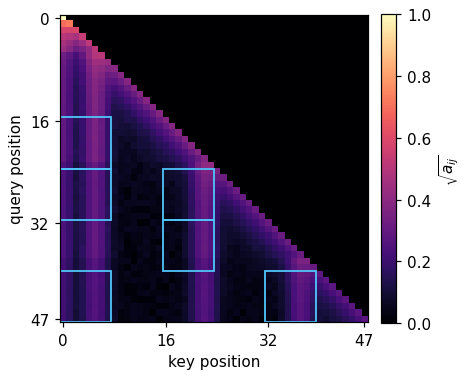
\includegraphics[width=0.8\linewidth]{figures/attention.png}
  \caption{Dense attention weights for one head of layer 18 on a 4k-token
  excerpt. Blocks selected by \textsc{Sieve} are outlined.}
  \label{fig:attention}
\end{figure}

\subsection{Ablations}

Removing the spread term $\sigma_i$ from the block score costs 2.1 points on
needle retrieval, and disabling selection reuse across layers increases
latency by 18\% with no change in accuracy. See \autoref{sec:analysis} for
why the spread term matters.

\section{Results}
\label{sec:results}

We evaluate on four long-context benchmarks: needle retrieval, multi-document
question answering, code completion over whole repositories, and long-form
summarisation. All models are 7B-parameter decoders fine-tuned at 32k tokens
and evaluated at up to 128k.

\begin{table}[ht]
  \centering
  \caption{Accuracy and keys read per query at 128k tokens. Higher accuracy is
  better; fewer keys is cheaper. Best sparse result in bold.}
  \label{tab:results}
  \begin{tabular}{lrrrr}
    \toprule
    Method        & Needle & Multi-doc QA & Repo code & Keys read \\
    \midrule
    Dense         & 99.1   & 71.4         & 58.2      & 131{,}072 \\
    Sliding window & 41.7  & 52.9         & 44.0      & 4{,}096   \\
    BigBird       & 88.3   & 63.0         & 51.6      & 12{,}288  \\
    Routing       & 95.6   & 68.1         & 55.9      & 16{,}384  \\
    \midrule
    \textsc{Sieve} ($k=8$)  & 97.8 & 69.9 & 56.7 & 6{,}144 \\
    \textsc{Sieve} ($k=16$) & \textbf{98.9} & \textbf{71.0} & \textbf{57.8} & 11{,}264 \\
    \bottomrule
  \end{tabular}
\end{table}

Table~\ref{tab:results} summarises the main comparison. \textsc{Sieve} with
$k = 16$ is within 0.4 points of dense attention on every task while reading
$11.6\times$ fewer keys. Sliding-window attention fails at needle retrieval,
as expected, because the answer is rarely local to the question.

\begin{figure}[ht]
  \centering
  %% Creator: Matplotlib, PGF backend
%%
%% To include the figure in your LaTeX document, write
%%   \input{<filename>.pgf}
%%
%% Make sure the required packages are loaded in your preamble
%%   \usepackage{pgf}
%%
%% Also ensure that all the required font packages are loaded; for instance,
%% the lmodern package is sometimes necessary when using math font.
%%   \usepackage{lmodern}
%%
%% Figures using additional raster images can only be included by \input if
%% they are in the same directory as the main LaTeX file. For loading figures
%% from other directories you can use the `import` package
%%   \usepackage{import}
%%
%% and then include the figures with
%%   \import{<path to file>}{<filename>.pgf}
%%
%% Matplotlib used the following preamble
%%   \def\mathdefault#1{#1}
%%   \everymath=\expandafter{\the\everymath\displaystyle}
%%   
%%   \ifdefined\pdftexversion\else  % non-pdftex case.
%%     \usepackage{fontspec}
%%     \setmainfont{DejaVuSerif.ttf}[Path=\detokenize{/Library/Frameworks/Python.framework/Versions/3.12/lib/python3.12/site-packages/matplotlib/mpl-data/fonts/ttf/}]
%%     \setsansfont{DejaVuSans.ttf}[Path=\detokenize{/Library/Frameworks/Python.framework/Versions/3.12/lib/python3.12/site-packages/matplotlib/mpl-data/fonts/ttf/}]
%%     \setmonofont{DejaVuSansMono.ttf}[Path=\detokenize{/Library/Frameworks/Python.framework/Versions/3.12/lib/python3.12/site-packages/matplotlib/mpl-data/fonts/ttf/}]
%%   \fi
%%   \makeatletter\@ifpackageloaded{underscore}{}{\usepackage[strings]{underscore}}\makeatother
%%
\begingroup%
\makeatletter%
\begin{pgfpicture}%
\pgfpathrectangle{\pgfpointorigin}{\pgfqpoint{4.600000in}{2.900000in}}%
\pgfusepath{use as bounding box, clip}%
\begin{pgfscope}%
\pgfsetbuttcap%
\pgfsetmiterjoin%
\definecolor{currentfill}{rgb}{1.000000,1.000000,1.000000}%
\pgfsetfillcolor{currentfill}%
\pgfsetlinewidth{0.000000pt}%
\definecolor{currentstroke}{rgb}{1.000000,1.000000,1.000000}%
\pgfsetstrokecolor{currentstroke}%
\pgfsetdash{}{0pt}%
\pgfpathmoveto{\pgfqpoint{0.000000in}{0.000000in}}%
\pgfpathlineto{\pgfqpoint{4.600000in}{0.000000in}}%
\pgfpathlineto{\pgfqpoint{4.600000in}{2.900000in}}%
\pgfpathlineto{\pgfqpoint{0.000000in}{2.900000in}}%
\pgfpathlineto{\pgfqpoint{0.000000in}{0.000000in}}%
\pgfpathclose%
\pgfusepath{fill}%
\end{pgfscope}%
\begin{pgfscope}%
\pgfsetbuttcap%
\pgfsetmiterjoin%
\definecolor{currentfill}{rgb}{1.000000,1.000000,1.000000}%
\pgfsetfillcolor{currentfill}%
\pgfsetlinewidth{0.000000pt}%
\definecolor{currentstroke}{rgb}{0.000000,0.000000,0.000000}%
\pgfsetstrokecolor{currentstroke}%
\pgfsetstrokeopacity{0.000000}%
\pgfsetdash{}{0pt}%
\pgfpathmoveto{\pgfqpoint{0.942108in}{0.582778in}}%
\pgfpathlineto{\pgfqpoint{4.450000in}{0.582778in}}%
\pgfpathlineto{\pgfqpoint{4.450000in}{2.750000in}}%
\pgfpathlineto{\pgfqpoint{0.942108in}{2.750000in}}%
\pgfpathlineto{\pgfqpoint{0.942108in}{0.582778in}}%
\pgfpathclose%
\pgfusepath{fill}%
\end{pgfscope}%
\begin{pgfscope}%
\pgfpathrectangle{\pgfqpoint{0.942108in}{0.582778in}}{\pgfqpoint{3.507892in}{2.167222in}}%
\pgfusepath{clip}%
\pgfsetbuttcap%
\pgfsetroundjoin%
\definecolor{currentfill}{rgb}{1.000000,0.584314,0.000000}%
\pgfsetfillcolor{currentfill}%
\pgfsetfillopacity{0.180000}%
\pgfsetlinewidth{0.000000pt}%
\definecolor{currentstroke}{rgb}{1.000000,0.584314,0.000000}%
\pgfsetstrokecolor{currentstroke}%
\pgfsetstrokeopacity{0.180000}%
\pgfsetdash{}{0pt}%
\pgfsys@defobject{currentmarker}{\pgfqpoint{1.101557in}{0.700885in}}{\pgfqpoint{4.290550in}{2.495498in}}{%
\pgfpathmoveto{\pgfqpoint{1.101557in}{2.495498in}}%
\pgfpathlineto{\pgfqpoint{1.101557in}{2.417550in}}%
\pgfpathlineto{\pgfqpoint{1.121488in}{2.374273in}}%
\pgfpathlineto{\pgfqpoint{1.141420in}{2.310227in}}%
\pgfpathlineto{\pgfqpoint{1.161351in}{2.287531in}}%
\pgfpathlineto{\pgfqpoint{1.181282in}{2.240011in}}%
\pgfpathlineto{\pgfqpoint{1.201213in}{2.215017in}}%
\pgfpathlineto{\pgfqpoint{1.221144in}{2.162805in}}%
\pgfpathlineto{\pgfqpoint{1.241076in}{2.119581in}}%
\pgfpathlineto{\pgfqpoint{1.261007in}{2.085505in}}%
\pgfpathlineto{\pgfqpoint{1.280938in}{2.050904in}}%
\pgfpathlineto{\pgfqpoint{1.300869in}{2.008160in}}%
\pgfpathlineto{\pgfqpoint{1.320800in}{1.976095in}}%
\pgfpathlineto{\pgfqpoint{1.340732in}{1.929877in}}%
\pgfpathlineto{\pgfqpoint{1.360663in}{1.904543in}}%
\pgfpathlineto{\pgfqpoint{1.380594in}{1.879047in}}%
\pgfpathlineto{\pgfqpoint{1.400525in}{1.856081in}}%
\pgfpathlineto{\pgfqpoint{1.420457in}{1.812893in}}%
\pgfpathlineto{\pgfqpoint{1.440388in}{1.777388in}}%
\pgfpathlineto{\pgfqpoint{1.460319in}{1.754407in}}%
\pgfpathlineto{\pgfqpoint{1.480250in}{1.722701in}}%
\pgfpathlineto{\pgfqpoint{1.500181in}{1.698938in}}%
\pgfpathlineto{\pgfqpoint{1.520113in}{1.664865in}}%
\pgfpathlineto{\pgfqpoint{1.540044in}{1.625673in}}%
\pgfpathlineto{\pgfqpoint{1.559975in}{1.601581in}}%
\pgfpathlineto{\pgfqpoint{1.579906in}{1.573959in}}%
\pgfpathlineto{\pgfqpoint{1.599837in}{1.548897in}}%
\pgfpathlineto{\pgfqpoint{1.619769in}{1.522375in}}%
\pgfpathlineto{\pgfqpoint{1.639700in}{1.488027in}}%
\pgfpathlineto{\pgfqpoint{1.659631in}{1.450840in}}%
\pgfpathlineto{\pgfqpoint{1.679562in}{1.441056in}}%
\pgfpathlineto{\pgfqpoint{1.699493in}{1.404633in}}%
\pgfpathlineto{\pgfqpoint{1.719425in}{1.402809in}}%
\pgfpathlineto{\pgfqpoint{1.739356in}{1.380364in}}%
\pgfpathlineto{\pgfqpoint{1.759287in}{1.342313in}}%
\pgfpathlineto{\pgfqpoint{1.779218in}{1.345331in}}%
\pgfpathlineto{\pgfqpoint{1.799149in}{1.327086in}}%
\pgfpathlineto{\pgfqpoint{1.819081in}{1.299820in}}%
\pgfpathlineto{\pgfqpoint{1.839012in}{1.296794in}}%
\pgfpathlineto{\pgfqpoint{1.858943in}{1.280513in}}%
\pgfpathlineto{\pgfqpoint{1.878874in}{1.231137in}}%
\pgfpathlineto{\pgfqpoint{1.898805in}{1.236844in}}%
\pgfpathlineto{\pgfqpoint{1.918737in}{1.213867in}}%
\pgfpathlineto{\pgfqpoint{1.938668in}{1.197274in}}%
\pgfpathlineto{\pgfqpoint{1.958599in}{1.186760in}}%
\pgfpathlineto{\pgfqpoint{1.978530in}{1.154095in}}%
\pgfpathlineto{\pgfqpoint{1.998462in}{1.140456in}}%
\pgfpathlineto{\pgfqpoint{2.018393in}{1.123469in}}%
\pgfpathlineto{\pgfqpoint{2.038324in}{1.110151in}}%
\pgfpathlineto{\pgfqpoint{2.058255in}{1.103458in}}%
\pgfpathlineto{\pgfqpoint{2.078186in}{1.075874in}}%
\pgfpathlineto{\pgfqpoint{2.098118in}{1.067387in}}%
\pgfpathlineto{\pgfqpoint{2.118049in}{1.072241in}}%
\pgfpathlineto{\pgfqpoint{2.137980in}{1.053360in}}%
\pgfpathlineto{\pgfqpoint{2.157911in}{1.046571in}}%
\pgfpathlineto{\pgfqpoint{2.177842in}{1.011003in}}%
\pgfpathlineto{\pgfqpoint{2.197774in}{1.011974in}}%
\pgfpathlineto{\pgfqpoint{2.217705in}{1.003878in}}%
\pgfpathlineto{\pgfqpoint{2.237636in}{0.999971in}}%
\pgfpathlineto{\pgfqpoint{2.257567in}{0.983480in}}%
\pgfpathlineto{\pgfqpoint{2.277498in}{0.990178in}}%
\pgfpathlineto{\pgfqpoint{2.297430in}{0.970365in}}%
\pgfpathlineto{\pgfqpoint{2.317361in}{0.962247in}}%
\pgfpathlineto{\pgfqpoint{2.337292in}{0.953582in}}%
\pgfpathlineto{\pgfqpoint{2.357223in}{0.952656in}}%
\pgfpathlineto{\pgfqpoint{2.377154in}{0.931985in}}%
\pgfpathlineto{\pgfqpoint{2.397086in}{0.941206in}}%
\pgfpathlineto{\pgfqpoint{2.417017in}{0.926623in}}%
\pgfpathlineto{\pgfqpoint{2.436948in}{0.916085in}}%
\pgfpathlineto{\pgfqpoint{2.456879in}{0.907859in}}%
\pgfpathlineto{\pgfqpoint{2.476810in}{0.906163in}}%
\pgfpathlineto{\pgfqpoint{2.496742in}{0.904850in}}%
\pgfpathlineto{\pgfqpoint{2.516673in}{0.897768in}}%
\pgfpathlineto{\pgfqpoint{2.536604in}{0.885615in}}%
\pgfpathlineto{\pgfqpoint{2.556535in}{0.885001in}}%
\pgfpathlineto{\pgfqpoint{2.576467in}{0.871282in}}%
\pgfpathlineto{\pgfqpoint{2.596398in}{0.877727in}}%
\pgfpathlineto{\pgfqpoint{2.616329in}{0.858941in}}%
\pgfpathlineto{\pgfqpoint{2.636260in}{0.832128in}}%
\pgfpathlineto{\pgfqpoint{2.656191in}{0.863177in}}%
\pgfpathlineto{\pgfqpoint{2.676123in}{0.845518in}}%
\pgfpathlineto{\pgfqpoint{2.696054in}{0.827485in}}%
\pgfpathlineto{\pgfqpoint{2.715985in}{0.833274in}}%
\pgfpathlineto{\pgfqpoint{2.735916in}{0.821827in}}%
\pgfpathlineto{\pgfqpoint{2.755847in}{0.848677in}}%
\pgfpathlineto{\pgfqpoint{2.775779in}{0.828111in}}%
\pgfpathlineto{\pgfqpoint{2.795710in}{0.802798in}}%
\pgfpathlineto{\pgfqpoint{2.815641in}{0.821040in}}%
\pgfpathlineto{\pgfqpoint{2.835572in}{0.807719in}}%
\pgfpathlineto{\pgfqpoint{2.855503in}{0.828004in}}%
\pgfpathlineto{\pgfqpoint{2.875435in}{0.794247in}}%
\pgfpathlineto{\pgfqpoint{2.895366in}{0.778763in}}%
\pgfpathlineto{\pgfqpoint{2.915297in}{0.799455in}}%
\pgfpathlineto{\pgfqpoint{2.935228in}{0.792266in}}%
\pgfpathlineto{\pgfqpoint{2.955159in}{0.788714in}}%
\pgfpathlineto{\pgfqpoint{2.975091in}{0.768414in}}%
\pgfpathlineto{\pgfqpoint{2.995022in}{0.791818in}}%
\pgfpathlineto{\pgfqpoint{3.014953in}{0.801711in}}%
\pgfpathlineto{\pgfqpoint{3.034884in}{0.763259in}}%
\pgfpathlineto{\pgfqpoint{3.054815in}{0.791773in}}%
\pgfpathlineto{\pgfqpoint{3.074747in}{0.772132in}}%
\pgfpathlineto{\pgfqpoint{3.094678in}{0.798798in}}%
\pgfpathlineto{\pgfqpoint{3.114609in}{0.777778in}}%
\pgfpathlineto{\pgfqpoint{3.134540in}{0.769560in}}%
\pgfpathlineto{\pgfqpoint{3.154472in}{0.780285in}}%
\pgfpathlineto{\pgfqpoint{3.174403in}{0.772687in}}%
\pgfpathlineto{\pgfqpoint{3.194334in}{0.759906in}}%
\pgfpathlineto{\pgfqpoint{3.214265in}{0.770844in}}%
\pgfpathlineto{\pgfqpoint{3.234196in}{0.757275in}}%
\pgfpathlineto{\pgfqpoint{3.254128in}{0.743228in}}%
\pgfpathlineto{\pgfqpoint{3.274059in}{0.778522in}}%
\pgfpathlineto{\pgfqpoint{3.293990in}{0.754145in}}%
\pgfpathlineto{\pgfqpoint{3.313921in}{0.750206in}}%
\pgfpathlineto{\pgfqpoint{3.333852in}{0.757868in}}%
\pgfpathlineto{\pgfqpoint{3.353784in}{0.738404in}}%
\pgfpathlineto{\pgfqpoint{3.373715in}{0.739117in}}%
\pgfpathlineto{\pgfqpoint{3.393646in}{0.746003in}}%
\pgfpathlineto{\pgfqpoint{3.413577in}{0.744622in}}%
\pgfpathlineto{\pgfqpoint{3.433508in}{0.749027in}}%
\pgfpathlineto{\pgfqpoint{3.453440in}{0.757690in}}%
\pgfpathlineto{\pgfqpoint{3.473371in}{0.741741in}}%
\pgfpathlineto{\pgfqpoint{3.493302in}{0.749682in}}%
\pgfpathlineto{\pgfqpoint{3.513233in}{0.749669in}}%
\pgfpathlineto{\pgfqpoint{3.533164in}{0.733162in}}%
\pgfpathlineto{\pgfqpoint{3.553096in}{0.744330in}}%
\pgfpathlineto{\pgfqpoint{3.573027in}{0.732720in}}%
\pgfpathlineto{\pgfqpoint{3.592958in}{0.750149in}}%
\pgfpathlineto{\pgfqpoint{3.612889in}{0.743789in}}%
\pgfpathlineto{\pgfqpoint{3.632821in}{0.739025in}}%
\pgfpathlineto{\pgfqpoint{3.652752in}{0.726028in}}%
\pgfpathlineto{\pgfqpoint{3.672683in}{0.738420in}}%
\pgfpathlineto{\pgfqpoint{3.692614in}{0.729817in}}%
\pgfpathlineto{\pgfqpoint{3.712545in}{0.742266in}}%
\pgfpathlineto{\pgfqpoint{3.732477in}{0.734287in}}%
\pgfpathlineto{\pgfqpoint{3.752408in}{0.727536in}}%
\pgfpathlineto{\pgfqpoint{3.772339in}{0.742233in}}%
\pgfpathlineto{\pgfqpoint{3.792270in}{0.739840in}}%
\pgfpathlineto{\pgfqpoint{3.812201in}{0.727793in}}%
\pgfpathlineto{\pgfqpoint{3.832133in}{0.742508in}}%
\pgfpathlineto{\pgfqpoint{3.852064in}{0.729337in}}%
\pgfpathlineto{\pgfqpoint{3.871995in}{0.728757in}}%
\pgfpathlineto{\pgfqpoint{3.891926in}{0.732009in}}%
\pgfpathlineto{\pgfqpoint{3.911857in}{0.724041in}}%
\pgfpathlineto{\pgfqpoint{3.931789in}{0.726280in}}%
\pgfpathlineto{\pgfqpoint{3.951720in}{0.728259in}}%
\pgfpathlineto{\pgfqpoint{3.971651in}{0.742106in}}%
\pgfpathlineto{\pgfqpoint{3.991582in}{0.741407in}}%
\pgfpathlineto{\pgfqpoint{4.011513in}{0.726273in}}%
\pgfpathlineto{\pgfqpoint{4.031445in}{0.741487in}}%
\pgfpathlineto{\pgfqpoint{4.051376in}{0.727374in}}%
\pgfpathlineto{\pgfqpoint{4.071307in}{0.730549in}}%
\pgfpathlineto{\pgfqpoint{4.091238in}{0.734355in}}%
\pgfpathlineto{\pgfqpoint{4.111169in}{0.729167in}}%
\pgfpathlineto{\pgfqpoint{4.131101in}{0.746147in}}%
\pgfpathlineto{\pgfqpoint{4.151032in}{0.728169in}}%
\pgfpathlineto{\pgfqpoint{4.170963in}{0.716167in}}%
\pgfpathlineto{\pgfqpoint{4.190894in}{0.736178in}}%
\pgfpathlineto{\pgfqpoint{4.210826in}{0.722074in}}%
\pgfpathlineto{\pgfqpoint{4.230757in}{0.722710in}}%
\pgfpathlineto{\pgfqpoint{4.250688in}{0.700885in}}%
\pgfpathlineto{\pgfqpoint{4.270619in}{0.732643in}}%
\pgfpathlineto{\pgfqpoint{4.290550in}{0.730954in}}%
\pgfpathlineto{\pgfqpoint{4.290550in}{0.799688in}}%
\pgfpathlineto{\pgfqpoint{4.290550in}{0.799688in}}%
\pgfpathlineto{\pgfqpoint{4.270619in}{0.801403in}}%
\pgfpathlineto{\pgfqpoint{4.250688in}{0.770748in}}%
\pgfpathlineto{\pgfqpoint{4.230757in}{0.791953in}}%
\pgfpathlineto{\pgfqpoint{4.210826in}{0.791423in}}%
\pgfpathlineto{\pgfqpoint{4.190894in}{0.805161in}}%
\pgfpathlineto{\pgfqpoint{4.170963in}{0.785882in}}%
\pgfpathlineto{\pgfqpoint{4.151032in}{0.797588in}}%
\pgfpathlineto{\pgfqpoint{4.131101in}{0.815081in}}%
\pgfpathlineto{\pgfqpoint{4.111169in}{0.798741in}}%
\pgfpathlineto{\pgfqpoint{4.091238in}{0.803858in}}%
\pgfpathlineto{\pgfqpoint{4.071307in}{0.800274in}}%
\pgfpathlineto{\pgfqpoint{4.051376in}{0.797302in}}%
\pgfpathlineto{\pgfqpoint{4.031445in}{0.811061in}}%
\pgfpathlineto{\pgfqpoint{4.011513in}{0.796444in}}%
\pgfpathlineto{\pgfqpoint{3.991582in}{0.811194in}}%
\pgfpathlineto{\pgfqpoint{3.971651in}{0.811979in}}%
\pgfpathlineto{\pgfqpoint{3.951720in}{0.798694in}}%
\pgfpathlineto{\pgfqpoint{3.931789in}{0.796894in}}%
\pgfpathlineto{\pgfqpoint{3.911857in}{0.794844in}}%
\pgfpathlineto{\pgfqpoint{3.891926in}{0.802669in}}%
\pgfpathlineto{\pgfqpoint{3.871995in}{0.799645in}}%
\pgfpathlineto{\pgfqpoint{3.852064in}{0.800329in}}%
\pgfpathlineto{\pgfqpoint{3.832133in}{0.813194in}}%
\pgfpathlineto{\pgfqpoint{3.812201in}{0.799092in}}%
\pgfpathlineto{\pgfqpoint{3.792270in}{0.810874in}}%
\pgfpathlineto{\pgfqpoint{3.772339in}{0.813321in}}%
\pgfpathlineto{\pgfqpoint{3.752408in}{0.799247in}}%
\pgfpathlineto{\pgfqpoint{3.732477in}{0.805914in}}%
\pgfpathlineto{\pgfqpoint{3.712545in}{0.813771in}}%
\pgfpathlineto{\pgfqpoint{3.692614in}{0.801882in}}%
\pgfpathlineto{\pgfqpoint{3.672683in}{0.810346in}}%
\pgfpathlineto{\pgfqpoint{3.652752in}{0.798521in}}%
\pgfpathlineto{\pgfqpoint{3.632821in}{0.811238in}}%
\pgfpathlineto{\pgfqpoint{3.612889in}{0.816000in}}%
\pgfpathlineto{\pgfqpoint{3.592958in}{0.822308in}}%
\pgfpathlineto{\pgfqpoint{3.573027in}{0.805630in}}%
\pgfpathlineto{\pgfqpoint{3.553096in}{0.817016in}}%
\pgfpathlineto{\pgfqpoint{3.533164in}{0.806398in}}%
\pgfpathlineto{\pgfqpoint{3.513233in}{0.822521in}}%
\pgfpathlineto{\pgfqpoint{3.493302in}{0.822712in}}%
\pgfpathlineto{\pgfqpoint{3.473371in}{0.815222in}}%
\pgfpathlineto{\pgfqpoint{3.453440in}{0.830816in}}%
\pgfpathlineto{\pgfqpoint{3.433508in}{0.822636in}}%
\pgfpathlineto{\pgfqpoint{3.413577in}{0.818575in}}%
\pgfpathlineto{\pgfqpoint{3.393646in}{0.820107in}}%
\pgfpathlineto{\pgfqpoint{3.373715in}{0.813661in}}%
\pgfpathlineto{\pgfqpoint{3.353784in}{0.813179in}}%
\pgfpathlineto{\pgfqpoint{3.333852in}{0.832181in}}%
\pgfpathlineto{\pgfqpoint{3.313921in}{0.824999in}}%
\pgfpathlineto{\pgfqpoint{3.293990in}{0.829020in}}%
\pgfpathlineto{\pgfqpoint{3.274059in}{0.852777in}}%
\pgfpathlineto{\pgfqpoint{3.254128in}{0.818936in}}%
\pgfpathlineto{\pgfqpoint{3.234196in}{0.832724in}}%
\pgfpathlineto{\pgfqpoint{3.214265in}{0.846057in}}%
\pgfpathlineto{\pgfqpoint{3.194334in}{0.835742in}}%
\pgfpathlineto{\pgfqpoint{3.174403in}{0.848322in}}%
\pgfpathlineto{\pgfqpoint{3.154472in}{0.855904in}}%
\pgfpathlineto{\pgfqpoint{3.134540in}{0.845812in}}%
\pgfpathlineto{\pgfqpoint{3.114609in}{0.854001in}}%
\pgfpathlineto{\pgfqpoint{3.094678in}{0.874546in}}%
\pgfpathlineto{\pgfqpoint{3.074747in}{0.849094in}}%
\pgfpathlineto{\pgfqpoint{3.054815in}{0.868314in}}%
\pgfpathlineto{\pgfqpoint{3.034884in}{0.841102in}}%
\pgfpathlineto{\pgfqpoint{3.014953in}{0.878467in}}%
\pgfpathlineto{\pgfqpoint{2.995022in}{0.869220in}}%
\pgfpathlineto{\pgfqpoint{2.975091in}{0.846961in}}%
\pgfpathlineto{\pgfqpoint{2.955159in}{0.866832in}}%
\pgfpathlineto{\pgfqpoint{2.935228in}{0.870569in}}%
\pgfpathlineto{\pgfqpoint{2.915297in}{0.877815in}}%
\pgfpathlineto{\pgfqpoint{2.895366in}{0.858204in}}%
\pgfpathlineto{\pgfqpoint{2.875435in}{0.873453in}}%
\pgfpathlineto{\pgfqpoint{2.855503in}{0.906316in}}%
\pgfpathlineto{\pgfqpoint{2.835572in}{0.887113in}}%
\pgfpathlineto{\pgfqpoint{2.815641in}{0.900295in}}%
\pgfpathlineto{\pgfqpoint{2.795710in}{0.883084in}}%
\pgfpathlineto{\pgfqpoint{2.775779in}{0.907824in}}%
\pgfpathlineto{\pgfqpoint{2.755847in}{0.928001in}}%
\pgfpathlineto{\pgfqpoint{2.735916in}{0.902521in}}%
\pgfpathlineto{\pgfqpoint{2.715985in}{0.913927in}}%
\pgfpathlineto{\pgfqpoint{2.696054in}{0.908748in}}%
\pgfpathlineto{\pgfqpoint{2.676123in}{0.926505in}}%
\pgfpathlineto{\pgfqpoint{2.656191in}{0.943908in}}%
\pgfpathlineto{\pgfqpoint{2.636260in}{0.914444in}}%
\pgfpathlineto{\pgfqpoint{2.616329in}{0.940665in}}%
\pgfpathlineto{\pgfqpoint{2.596398in}{0.959170in}}%
\pgfpathlineto{\pgfqpoint{2.576467in}{0.953405in}}%
\pgfpathlineto{\pgfqpoint{2.556535in}{0.967048in}}%
\pgfpathlineto{\pgfqpoint{2.536604in}{0.968090in}}%
\pgfpathlineto{\pgfqpoint{2.516673in}{0.980241in}}%
\pgfpathlineto{\pgfqpoint{2.496742in}{0.987521in}}%
\pgfpathlineto{\pgfqpoint{2.476810in}{0.989259in}}%
\pgfpathlineto{\pgfqpoint{2.456879in}{0.991377in}}%
\pgfpathlineto{\pgfqpoint{2.436948in}{0.999779in}}%
\pgfpathlineto{\pgfqpoint{2.417017in}{1.010414in}}%
\pgfpathlineto{\pgfqpoint{2.397086in}{1.024943in}}%
\pgfpathlineto{\pgfqpoint{2.377154in}{1.016602in}}%
\pgfpathlineto{\pgfqpoint{2.357223in}{1.036996in}}%
\pgfpathlineto{\pgfqpoint{2.337292in}{1.038425in}}%
\pgfpathlineto{\pgfqpoint{2.317361in}{1.047298in}}%
\pgfpathlineto{\pgfqpoint{2.297430in}{1.055655in}}%
\pgfpathlineto{\pgfqpoint{2.277498in}{1.075254in}}%
\pgfpathlineto{\pgfqpoint{2.257567in}{1.069397in}}%
\pgfpathlineto{\pgfqpoint{2.237636in}{1.085821in}}%
\pgfpathlineto{\pgfqpoint{2.217705in}{1.090169in}}%
\pgfpathlineto{\pgfqpoint{2.197774in}{1.098549in}}%
\pgfpathlineto{\pgfqpoint{2.177842in}{1.098235in}}%
\pgfpathlineto{\pgfqpoint{2.157911in}{1.133003in}}%
\pgfpathlineto{\pgfqpoint{2.137980in}{1.140154in}}%
\pgfpathlineto{\pgfqpoint{2.118049in}{1.158921in}}%
\pgfpathlineto{\pgfqpoint{2.098118in}{1.154917in}}%
\pgfpathlineto{\pgfqpoint{2.078186in}{1.163727in}}%
\pgfpathlineto{\pgfqpoint{2.058255in}{1.190870in}}%
\pgfpathlineto{\pgfqpoint{2.038324in}{1.197977in}}%
\pgfpathlineto{\pgfqpoint{2.018393in}{1.211449in}}%
\pgfpathlineto{\pgfqpoint{1.998462in}{1.228450in}}%
\pgfpathlineto{\pgfqpoint{1.978530in}{1.242249in}}%
\pgfpathlineto{\pgfqpoint{1.958599in}{1.274310in}}%
\pgfpathlineto{\pgfqpoint{1.938668in}{1.285127in}}%
\pgfpathlineto{\pgfqpoint{1.918737in}{1.301787in}}%
\pgfpathlineto{\pgfqpoint{1.898805in}{1.324581in}}%
\pgfpathlineto{\pgfqpoint{1.878874in}{1.319867in}}%
\pgfpathlineto{\pgfqpoint{1.858943in}{1.368003in}}%
\pgfpathlineto{\pgfqpoint{1.839012in}{1.384399in}}%
\pgfpathlineto{\pgfqpoint{1.819081in}{1.388088in}}%
\pgfpathlineto{\pgfqpoint{1.799149in}{1.415041in}}%
\pgfpathlineto{\pgfqpoint{1.779218in}{1.433350in}}%
\pgfpathlineto{\pgfqpoint{1.759287in}{1.431274in}}%
\pgfpathlineto{\pgfqpoint{1.739356in}{1.468597in}}%
\pgfpathlineto{\pgfqpoint{1.719425in}{1.490963in}}%
\pgfpathlineto{\pgfqpoint{1.699493in}{1.493559in}}%
\pgfpathlineto{\pgfqpoint{1.679562in}{1.529349in}}%
\pgfpathlineto{\pgfqpoint{1.659631in}{1.539599in}}%
\pgfpathlineto{\pgfqpoint{1.639700in}{1.576142in}}%
\pgfpathlineto{\pgfqpoint{1.619769in}{1.609975in}}%
\pgfpathlineto{\pgfqpoint{1.599837in}{1.636309in}}%
\pgfpathlineto{\pgfqpoint{1.579906in}{1.661251in}}%
\pgfpathlineto{\pgfqpoint{1.559975in}{1.688660in}}%
\pgfpathlineto{\pgfqpoint{1.540044in}{1.712691in}}%
\pgfpathlineto{\pgfqpoint{1.520113in}{1.751226in}}%
\pgfpathlineto{\pgfqpoint{1.500181in}{1.784859in}}%
\pgfpathlineto{\pgfqpoint{1.480250in}{1.808602in}}%
\pgfpathlineto{\pgfqpoint{1.460319in}{1.839982in}}%
\pgfpathlineto{\pgfqpoint{1.440388in}{1.862992in}}%
\pgfpathlineto{\pgfqpoint{1.420457in}{1.898040in}}%
\pgfpathlineto{\pgfqpoint{1.400525in}{1.940483in}}%
\pgfpathlineto{\pgfqpoint{1.380594in}{1.963505in}}%
\pgfpathlineto{\pgfqpoint{1.360663in}{1.988967in}}%
\pgfpathlineto{\pgfqpoint{1.340732in}{2.014282in}}%
\pgfpathlineto{\pgfqpoint{1.320800in}{2.059679in}}%
\pgfpathlineto{\pgfqpoint{1.300869in}{2.091484in}}%
\pgfpathlineto{\pgfqpoint{1.280938in}{2.133567in}}%
\pgfpathlineto{\pgfqpoint{1.261007in}{2.167830in}}%
\pgfpathlineto{\pgfqpoint{1.241076in}{2.201598in}}%
\pgfpathlineto{\pgfqpoint{1.221144in}{2.244179in}}%
\pgfpathlineto{\pgfqpoint{1.201213in}{2.295425in}}%
\pgfpathlineto{\pgfqpoint{1.181282in}{2.320481in}}%
\pgfpathlineto{\pgfqpoint{1.161351in}{2.367236in}}%
\pgfpathlineto{\pgfqpoint{1.141420in}{2.390093in}}%
\pgfpathlineto{\pgfqpoint{1.121488in}{2.452793in}}%
\pgfpathlineto{\pgfqpoint{1.101557in}{2.495498in}}%
\pgfpathlineto{\pgfqpoint{1.101557in}{2.495498in}}%
\pgfpathclose%
\pgfusepath{fill}%
}%
\begin{pgfscope}%
\pgfsys@transformshift{0.000000in}{0.000000in}%
\pgfsys@useobject{currentmarker}{}%
\end{pgfscope}%
\end{pgfscope}%
\begin{pgfscope}%
\pgfpathrectangle{\pgfqpoint{0.942108in}{0.582778in}}{\pgfqpoint{3.507892in}{2.167222in}}%
\pgfusepath{clip}%
\pgfsetrectcap%
\pgfsetroundjoin%
\pgfsetlinewidth{0.602250pt}%
\definecolor{currentstroke}{rgb}{0.819608,0.819608,0.839216}%
\pgfsetstrokecolor{currentstroke}%
\pgfsetdash{}{0pt}%
\pgfpathmoveto{\pgfqpoint{1.101557in}{0.582778in}}%
\pgfpathlineto{\pgfqpoint{1.101557in}{2.750000in}}%
\pgfusepath{stroke}%
\end{pgfscope}%
\begin{pgfscope}%
\pgfsetbuttcap%
\pgfsetroundjoin%
\definecolor{currentfill}{rgb}{0.000000,0.000000,0.000000}%
\pgfsetfillcolor{currentfill}%
\pgfsetlinewidth{0.803000pt}%
\definecolor{currentstroke}{rgb}{0.000000,0.000000,0.000000}%
\pgfsetstrokecolor{currentstroke}%
\pgfsetdash{}{0pt}%
\pgfsys@defobject{currentmarker}{\pgfqpoint{0.000000in}{-0.048611in}}{\pgfqpoint{0.000000in}{0.000000in}}{%
\pgfpathmoveto{\pgfqpoint{0.000000in}{0.000000in}}%
\pgfpathlineto{\pgfqpoint{0.000000in}{-0.048611in}}%
\pgfusepath{stroke,fill}%
}%
\begin{pgfscope}%
\pgfsys@transformshift{1.101557in}{0.582778in}%
\pgfsys@useobject{currentmarker}{}%
\end{pgfscope}%
\end{pgfscope}%
\begin{pgfscope}%
\definecolor{textcolor}{rgb}{0.000000,0.000000,0.000000}%
\pgfsetstrokecolor{textcolor}%
\pgfsetfillcolor{textcolor}%
\pgftext[x=1.101557in,y=0.485556in,,top]{\color{textcolor}{\sffamily\fontsize{10.000000}{12.000000}\selectfont\catcode`\^=\active\def^{\ifmmode\sp\else\^{}\fi}\catcode`\%=\active\def%{\%}0}}%
\end{pgfscope}%
\begin{pgfscope}%
\pgfpathrectangle{\pgfqpoint{0.942108in}{0.582778in}}{\pgfqpoint{3.507892in}{2.167222in}}%
\pgfusepath{clip}%
\pgfsetrectcap%
\pgfsetroundjoin%
\pgfsetlinewidth{0.602250pt}%
\definecolor{currentstroke}{rgb}{0.819608,0.819608,0.839216}%
\pgfsetstrokecolor{currentstroke}%
\pgfsetdash{}{0pt}%
\pgfpathmoveto{\pgfqpoint{1.898805in}{0.582778in}}%
\pgfpathlineto{\pgfqpoint{1.898805in}{2.750000in}}%
\pgfusepath{stroke}%
\end{pgfscope}%
\begin{pgfscope}%
\pgfsetbuttcap%
\pgfsetroundjoin%
\definecolor{currentfill}{rgb}{0.000000,0.000000,0.000000}%
\pgfsetfillcolor{currentfill}%
\pgfsetlinewidth{0.803000pt}%
\definecolor{currentstroke}{rgb}{0.000000,0.000000,0.000000}%
\pgfsetstrokecolor{currentstroke}%
\pgfsetdash{}{0pt}%
\pgfsys@defobject{currentmarker}{\pgfqpoint{0.000000in}{-0.048611in}}{\pgfqpoint{0.000000in}{0.000000in}}{%
\pgfpathmoveto{\pgfqpoint{0.000000in}{0.000000in}}%
\pgfpathlineto{\pgfqpoint{0.000000in}{-0.048611in}}%
\pgfusepath{stroke,fill}%
}%
\begin{pgfscope}%
\pgfsys@transformshift{1.898805in}{0.582778in}%
\pgfsys@useobject{currentmarker}{}%
\end{pgfscope}%
\end{pgfscope}%
\begin{pgfscope}%
\definecolor{textcolor}{rgb}{0.000000,0.000000,0.000000}%
\pgfsetstrokecolor{textcolor}%
\pgfsetfillcolor{textcolor}%
\pgftext[x=1.898805in,y=0.485556in,,top]{\color{textcolor}{\sffamily\fontsize{10.000000}{12.000000}\selectfont\catcode`\^=\active\def^{\ifmmode\sp\else\^{}\fi}\catcode`\%=\active\def%{\%}5k}}%
\end{pgfscope}%
\begin{pgfscope}%
\pgfpathrectangle{\pgfqpoint{0.942108in}{0.582778in}}{\pgfqpoint{3.507892in}{2.167222in}}%
\pgfusepath{clip}%
\pgfsetrectcap%
\pgfsetroundjoin%
\pgfsetlinewidth{0.602250pt}%
\definecolor{currentstroke}{rgb}{0.819608,0.819608,0.839216}%
\pgfsetstrokecolor{currentstroke}%
\pgfsetdash{}{0pt}%
\pgfpathmoveto{\pgfqpoint{2.696054in}{0.582778in}}%
\pgfpathlineto{\pgfqpoint{2.696054in}{2.750000in}}%
\pgfusepath{stroke}%
\end{pgfscope}%
\begin{pgfscope}%
\pgfsetbuttcap%
\pgfsetroundjoin%
\definecolor{currentfill}{rgb}{0.000000,0.000000,0.000000}%
\pgfsetfillcolor{currentfill}%
\pgfsetlinewidth{0.803000pt}%
\definecolor{currentstroke}{rgb}{0.000000,0.000000,0.000000}%
\pgfsetstrokecolor{currentstroke}%
\pgfsetdash{}{0pt}%
\pgfsys@defobject{currentmarker}{\pgfqpoint{0.000000in}{-0.048611in}}{\pgfqpoint{0.000000in}{0.000000in}}{%
\pgfpathmoveto{\pgfqpoint{0.000000in}{0.000000in}}%
\pgfpathlineto{\pgfqpoint{0.000000in}{-0.048611in}}%
\pgfusepath{stroke,fill}%
}%
\begin{pgfscope}%
\pgfsys@transformshift{2.696054in}{0.582778in}%
\pgfsys@useobject{currentmarker}{}%
\end{pgfscope}%
\end{pgfscope}%
\begin{pgfscope}%
\definecolor{textcolor}{rgb}{0.000000,0.000000,0.000000}%
\pgfsetstrokecolor{textcolor}%
\pgfsetfillcolor{textcolor}%
\pgftext[x=2.696054in,y=0.485556in,,top]{\color{textcolor}{\sffamily\fontsize{10.000000}{12.000000}\selectfont\catcode`\^=\active\def^{\ifmmode\sp\else\^{}\fi}\catcode`\%=\active\def%{\%}10k}}%
\end{pgfscope}%
\begin{pgfscope}%
\pgfpathrectangle{\pgfqpoint{0.942108in}{0.582778in}}{\pgfqpoint{3.507892in}{2.167222in}}%
\pgfusepath{clip}%
\pgfsetrectcap%
\pgfsetroundjoin%
\pgfsetlinewidth{0.602250pt}%
\definecolor{currentstroke}{rgb}{0.819608,0.819608,0.839216}%
\pgfsetstrokecolor{currentstroke}%
\pgfsetdash{}{0pt}%
\pgfpathmoveto{\pgfqpoint{3.493302in}{0.582778in}}%
\pgfpathlineto{\pgfqpoint{3.493302in}{2.750000in}}%
\pgfusepath{stroke}%
\end{pgfscope}%
\begin{pgfscope}%
\pgfsetbuttcap%
\pgfsetroundjoin%
\definecolor{currentfill}{rgb}{0.000000,0.000000,0.000000}%
\pgfsetfillcolor{currentfill}%
\pgfsetlinewidth{0.803000pt}%
\definecolor{currentstroke}{rgb}{0.000000,0.000000,0.000000}%
\pgfsetstrokecolor{currentstroke}%
\pgfsetdash{}{0pt}%
\pgfsys@defobject{currentmarker}{\pgfqpoint{0.000000in}{-0.048611in}}{\pgfqpoint{0.000000in}{0.000000in}}{%
\pgfpathmoveto{\pgfqpoint{0.000000in}{0.000000in}}%
\pgfpathlineto{\pgfqpoint{0.000000in}{-0.048611in}}%
\pgfusepath{stroke,fill}%
}%
\begin{pgfscope}%
\pgfsys@transformshift{3.493302in}{0.582778in}%
\pgfsys@useobject{currentmarker}{}%
\end{pgfscope}%
\end{pgfscope}%
\begin{pgfscope}%
\definecolor{textcolor}{rgb}{0.000000,0.000000,0.000000}%
\pgfsetstrokecolor{textcolor}%
\pgfsetfillcolor{textcolor}%
\pgftext[x=3.493302in,y=0.485556in,,top]{\color{textcolor}{\sffamily\fontsize{10.000000}{12.000000}\selectfont\catcode`\^=\active\def^{\ifmmode\sp\else\^{}\fi}\catcode`\%=\active\def%{\%}15k}}%
\end{pgfscope}%
\begin{pgfscope}%
\pgfpathrectangle{\pgfqpoint{0.942108in}{0.582778in}}{\pgfqpoint{3.507892in}{2.167222in}}%
\pgfusepath{clip}%
\pgfsetrectcap%
\pgfsetroundjoin%
\pgfsetlinewidth{0.602250pt}%
\definecolor{currentstroke}{rgb}{0.819608,0.819608,0.839216}%
\pgfsetstrokecolor{currentstroke}%
\pgfsetdash{}{0pt}%
\pgfpathmoveto{\pgfqpoint{4.290550in}{0.582778in}}%
\pgfpathlineto{\pgfqpoint{4.290550in}{2.750000in}}%
\pgfusepath{stroke}%
\end{pgfscope}%
\begin{pgfscope}%
\pgfsetbuttcap%
\pgfsetroundjoin%
\definecolor{currentfill}{rgb}{0.000000,0.000000,0.000000}%
\pgfsetfillcolor{currentfill}%
\pgfsetlinewidth{0.803000pt}%
\definecolor{currentstroke}{rgb}{0.000000,0.000000,0.000000}%
\pgfsetstrokecolor{currentstroke}%
\pgfsetdash{}{0pt}%
\pgfsys@defobject{currentmarker}{\pgfqpoint{0.000000in}{-0.048611in}}{\pgfqpoint{0.000000in}{0.000000in}}{%
\pgfpathmoveto{\pgfqpoint{0.000000in}{0.000000in}}%
\pgfpathlineto{\pgfqpoint{0.000000in}{-0.048611in}}%
\pgfusepath{stroke,fill}%
}%
\begin{pgfscope}%
\pgfsys@transformshift{4.290550in}{0.582778in}%
\pgfsys@useobject{currentmarker}{}%
\end{pgfscope}%
\end{pgfscope}%
\begin{pgfscope}%
\definecolor{textcolor}{rgb}{0.000000,0.000000,0.000000}%
\pgfsetstrokecolor{textcolor}%
\pgfsetfillcolor{textcolor}%
\pgftext[x=4.290550in,y=0.485556in,,top]{\color{textcolor}{\sffamily\fontsize{10.000000}{12.000000}\selectfont\catcode`\^=\active\def^{\ifmmode\sp\else\^{}\fi}\catcode`\%=\active\def%{\%}20k}}%
\end{pgfscope}%
\begin{pgfscope}%
\definecolor{textcolor}{rgb}{0.000000,0.000000,0.000000}%
\pgfsetstrokecolor{textcolor}%
\pgfsetfillcolor{textcolor}%
\pgftext[x=2.696054in,y=0.329200in,,top]{\color{textcolor}{\sffamily\fontsize{10.000000}{12.000000}\selectfont\catcode`\^=\active\def^{\ifmmode\sp\else\^{}\fi}\catcode`\%=\active\def%{\%}training step}}%
\end{pgfscope}%
\begin{pgfscope}%
\pgfsetbuttcap%
\pgfsetroundjoin%
\definecolor{currentfill}{rgb}{0.000000,0.000000,0.000000}%
\pgfsetfillcolor{currentfill}%
\pgfsetlinewidth{0.602250pt}%
\definecolor{currentstroke}{rgb}{0.000000,0.000000,0.000000}%
\pgfsetstrokecolor{currentstroke}%
\pgfsetdash{}{0pt}%
\pgfsys@defobject{currentmarker}{\pgfqpoint{-0.027778in}{0.000000in}}{\pgfqpoint{-0.000000in}{0.000000in}}{%
\pgfpathmoveto{\pgfqpoint{-0.000000in}{0.000000in}}%
\pgfpathlineto{\pgfqpoint{-0.027778in}{0.000000in}}%
\pgfusepath{stroke,fill}%
}%
\begin{pgfscope}%
\pgfsys@transformshift{0.942108in}{0.806278in}%
\pgfsys@useobject{currentmarker}{}%
\end{pgfscope}%
\end{pgfscope}%
\begin{pgfscope}%
\definecolor{textcolor}{rgb}{0.000000,0.000000,0.000000}%
\pgfsetstrokecolor{textcolor}%
\pgfsetfillcolor{textcolor}%
\pgftext[x=0.498790in, y=0.750118in, left, base]{\color{textcolor}{\sffamily\fontsize{10.000000}{12.000000}\selectfont\catcode`\^=\active\def^{\ifmmode\sp\else\^{}\fi}\catcode`\%=\active\def%{\%}$\mathdefault{2\times10^{0}}$}}%
\end{pgfscope}%
\begin{pgfscope}%
\pgfsetbuttcap%
\pgfsetroundjoin%
\definecolor{currentfill}{rgb}{0.000000,0.000000,0.000000}%
\pgfsetfillcolor{currentfill}%
\pgfsetlinewidth{0.602250pt}%
\definecolor{currentstroke}{rgb}{0.000000,0.000000,0.000000}%
\pgfsetstrokecolor{currentstroke}%
\pgfsetdash{}{0pt}%
\pgfsys@defobject{currentmarker}{\pgfqpoint{-0.027778in}{0.000000in}}{\pgfqpoint{-0.000000in}{0.000000in}}{%
\pgfpathmoveto{\pgfqpoint{-0.000000in}{0.000000in}}%
\pgfpathlineto{\pgfqpoint{-0.027778in}{0.000000in}}%
\pgfusepath{stroke,fill}%
}%
\begin{pgfscope}%
\pgfsys@transformshift{0.942108in}{1.666389in}%
\pgfsys@useobject{currentmarker}{}%
\end{pgfscope}%
\end{pgfscope}%
\begin{pgfscope}%
\definecolor{textcolor}{rgb}{0.000000,0.000000,0.000000}%
\pgfsetstrokecolor{textcolor}%
\pgfsetfillcolor{textcolor}%
\pgftext[x=0.498790in, y=1.610229in, left, base]{\color{textcolor}{\sffamily\fontsize{10.000000}{12.000000}\selectfont\catcode`\^=\active\def^{\ifmmode\sp\else\^{}\fi}\catcode`\%=\active\def%{\%}$\mathdefault{3\times10^{0}}$}}%
\end{pgfscope}%
\begin{pgfscope}%
\pgfsetbuttcap%
\pgfsetroundjoin%
\definecolor{currentfill}{rgb}{0.000000,0.000000,0.000000}%
\pgfsetfillcolor{currentfill}%
\pgfsetlinewidth{0.602250pt}%
\definecolor{currentstroke}{rgb}{0.000000,0.000000,0.000000}%
\pgfsetstrokecolor{currentstroke}%
\pgfsetdash{}{0pt}%
\pgfsys@defobject{currentmarker}{\pgfqpoint{-0.027778in}{0.000000in}}{\pgfqpoint{-0.000000in}{0.000000in}}{%
\pgfpathmoveto{\pgfqpoint{-0.000000in}{0.000000in}}%
\pgfpathlineto{\pgfqpoint{-0.027778in}{0.000000in}}%
\pgfusepath{stroke,fill}%
}%
\begin{pgfscope}%
\pgfsys@transformshift{0.942108in}{2.276647in}%
\pgfsys@useobject{currentmarker}{}%
\end{pgfscope}%
\end{pgfscope}%
\begin{pgfscope}%
\definecolor{textcolor}{rgb}{0.000000,0.000000,0.000000}%
\pgfsetstrokecolor{textcolor}%
\pgfsetfillcolor{textcolor}%
\pgftext[x=0.498790in, y=2.220487in, left, base]{\color{textcolor}{\sffamily\fontsize{10.000000}{12.000000}\selectfont\catcode`\^=\active\def^{\ifmmode\sp\else\^{}\fi}\catcode`\%=\active\def%{\%}$\mathdefault{4\times10^{0}}$}}%
\end{pgfscope}%
\begin{pgfscope}%
\pgfsetbuttcap%
\pgfsetroundjoin%
\definecolor{currentfill}{rgb}{0.000000,0.000000,0.000000}%
\pgfsetfillcolor{currentfill}%
\pgfsetlinewidth{0.602250pt}%
\definecolor{currentstroke}{rgb}{0.000000,0.000000,0.000000}%
\pgfsetstrokecolor{currentstroke}%
\pgfsetdash{}{0pt}%
\pgfsys@defobject{currentmarker}{\pgfqpoint{-0.027778in}{0.000000in}}{\pgfqpoint{-0.000000in}{0.000000in}}{%
\pgfpathmoveto{\pgfqpoint{-0.000000in}{0.000000in}}%
\pgfpathlineto{\pgfqpoint{-0.027778in}{0.000000in}}%
\pgfusepath{stroke,fill}%
}%
\begin{pgfscope}%
\pgfsys@transformshift{0.942108in}{2.750000in}%
\pgfsys@useobject{currentmarker}{}%
\end{pgfscope}%
\end{pgfscope}%
\begin{pgfscope}%
\definecolor{textcolor}{rgb}{0.000000,0.000000,0.000000}%
\pgfsetstrokecolor{textcolor}%
\pgfsetfillcolor{textcolor}%
\pgftext[x=0.443235in,y=1.666389in,,bottom,rotate=90.000000]{\color{textcolor}{\sffamily\fontsize{10.000000}{12.000000}\selectfont\catcode`\^=\active\def^{\ifmmode\sp\else\^{}\fi}\catcode`\%=\active\def%{\%}validation loss $\ell$}}%
\end{pgfscope}%
\begin{pgfscope}%
\pgfpathrectangle{\pgfqpoint{0.942108in}{0.582778in}}{\pgfqpoint{3.507892in}{2.167222in}}%
\pgfusepath{clip}%
\pgfsetrectcap%
\pgfsetroundjoin%
\pgfsetlinewidth{1.405250pt}%
\definecolor{currentstroke}{rgb}{0.000000,0.478431,1.000000}%
\pgfsetstrokecolor{currentstroke}%
\pgfsetdash{}{0pt}%
\pgfpathmoveto{\pgfqpoint{1.101557in}{2.435375in}}%
\pgfpathlineto{\pgfqpoint{1.121488in}{2.394885in}}%
\pgfpathlineto{\pgfqpoint{1.181282in}{2.252099in}}%
\pgfpathlineto{\pgfqpoint{1.201213in}{2.213736in}}%
\pgfpathlineto{\pgfqpoint{1.221144in}{2.187594in}}%
\pgfpathlineto{\pgfqpoint{1.241076in}{2.150292in}}%
\pgfpathlineto{\pgfqpoint{1.261007in}{2.101742in}}%
\pgfpathlineto{\pgfqpoint{1.280938in}{2.066257in}}%
\pgfpathlineto{\pgfqpoint{1.300869in}{2.016278in}}%
\pgfpathlineto{\pgfqpoint{1.340732in}{1.947505in}}%
\pgfpathlineto{\pgfqpoint{1.360663in}{1.901770in}}%
\pgfpathlineto{\pgfqpoint{1.380594in}{1.867160in}}%
\pgfpathlineto{\pgfqpoint{1.400525in}{1.840680in}}%
\pgfpathlineto{\pgfqpoint{1.440388in}{1.765522in}}%
\pgfpathlineto{\pgfqpoint{1.460319in}{1.744407in}}%
\pgfpathlineto{\pgfqpoint{1.480250in}{1.708155in}}%
\pgfpathlineto{\pgfqpoint{1.500181in}{1.687550in}}%
\pgfpathlineto{\pgfqpoint{1.520113in}{1.649813in}}%
\pgfpathlineto{\pgfqpoint{1.540044in}{1.618430in}}%
\pgfpathlineto{\pgfqpoint{1.559975in}{1.593512in}}%
\pgfpathlineto{\pgfqpoint{1.599837in}{1.532593in}}%
\pgfpathlineto{\pgfqpoint{1.619769in}{1.508560in}}%
\pgfpathlineto{\pgfqpoint{1.639700in}{1.492553in}}%
\pgfpathlineto{\pgfqpoint{1.659631in}{1.466952in}}%
\pgfpathlineto{\pgfqpoint{1.679562in}{1.448209in}}%
\pgfpathlineto{\pgfqpoint{1.699493in}{1.399677in}}%
\pgfpathlineto{\pgfqpoint{1.719425in}{1.387858in}}%
\pgfpathlineto{\pgfqpoint{1.739356in}{1.365486in}}%
\pgfpathlineto{\pgfqpoint{1.759287in}{1.348969in}}%
\pgfpathlineto{\pgfqpoint{1.779218in}{1.322659in}}%
\pgfpathlineto{\pgfqpoint{1.799149in}{1.301790in}}%
\pgfpathlineto{\pgfqpoint{1.819081in}{1.293360in}}%
\pgfpathlineto{\pgfqpoint{1.839012in}{1.268952in}}%
\pgfpathlineto{\pgfqpoint{1.858943in}{1.238505in}}%
\pgfpathlineto{\pgfqpoint{1.878874in}{1.242585in}}%
\pgfpathlineto{\pgfqpoint{1.898805in}{1.222172in}}%
\pgfpathlineto{\pgfqpoint{1.918737in}{1.191258in}}%
\pgfpathlineto{\pgfqpoint{1.938668in}{1.187403in}}%
\pgfpathlineto{\pgfqpoint{1.958599in}{1.157439in}}%
\pgfpathlineto{\pgfqpoint{1.978530in}{1.158769in}}%
\pgfpathlineto{\pgfqpoint{1.998462in}{1.131742in}}%
\pgfpathlineto{\pgfqpoint{2.018393in}{1.111962in}}%
\pgfpathlineto{\pgfqpoint{2.038324in}{1.101862in}}%
\pgfpathlineto{\pgfqpoint{2.058255in}{1.084719in}}%
\pgfpathlineto{\pgfqpoint{2.078186in}{1.080346in}}%
\pgfpathlineto{\pgfqpoint{2.118049in}{1.053961in}}%
\pgfpathlineto{\pgfqpoint{2.137980in}{1.036651in}}%
\pgfpathlineto{\pgfqpoint{2.157911in}{0.996395in}}%
\pgfpathlineto{\pgfqpoint{2.177842in}{1.020039in}}%
\pgfpathlineto{\pgfqpoint{2.197774in}{0.990939in}}%
\pgfpathlineto{\pgfqpoint{2.217705in}{1.000337in}}%
\pgfpathlineto{\pgfqpoint{2.237636in}{0.998463in}}%
\pgfpathlineto{\pgfqpoint{2.257567in}{0.980914in}}%
\pgfpathlineto{\pgfqpoint{2.277498in}{0.965447in}}%
\pgfpathlineto{\pgfqpoint{2.297430in}{0.958349in}}%
\pgfpathlineto{\pgfqpoint{2.317361in}{0.950059in}}%
\pgfpathlineto{\pgfqpoint{2.337292in}{0.937796in}}%
\pgfpathlineto{\pgfqpoint{2.357223in}{0.929347in}}%
\pgfpathlineto{\pgfqpoint{2.377154in}{0.918358in}}%
\pgfpathlineto{\pgfqpoint{2.397086in}{0.930216in}}%
\pgfpathlineto{\pgfqpoint{2.417017in}{0.911854in}}%
\pgfpathlineto{\pgfqpoint{2.436948in}{0.913712in}}%
\pgfpathlineto{\pgfqpoint{2.456879in}{0.895838in}}%
\pgfpathlineto{\pgfqpoint{2.476810in}{0.892230in}}%
\pgfpathlineto{\pgfqpoint{2.496742in}{0.883672in}}%
\pgfpathlineto{\pgfqpoint{2.516673in}{0.883354in}}%
\pgfpathlineto{\pgfqpoint{2.536604in}{0.880770in}}%
\pgfpathlineto{\pgfqpoint{2.556535in}{0.869735in}}%
\pgfpathlineto{\pgfqpoint{2.576467in}{0.855924in}}%
\pgfpathlineto{\pgfqpoint{2.596398in}{0.849684in}}%
\pgfpathlineto{\pgfqpoint{2.616329in}{0.866702in}}%
\pgfpathlineto{\pgfqpoint{2.636260in}{0.844248in}}%
\pgfpathlineto{\pgfqpoint{2.656191in}{0.839421in}}%
\pgfpathlineto{\pgfqpoint{2.676123in}{0.850674in}}%
\pgfpathlineto{\pgfqpoint{2.696054in}{0.842874in}}%
\pgfpathlineto{\pgfqpoint{2.715985in}{0.833657in}}%
\pgfpathlineto{\pgfqpoint{2.735916in}{0.821200in}}%
\pgfpathlineto{\pgfqpoint{2.755847in}{0.841798in}}%
\pgfpathlineto{\pgfqpoint{2.775779in}{0.820568in}}%
\pgfpathlineto{\pgfqpoint{2.795710in}{0.818278in}}%
\pgfpathlineto{\pgfqpoint{2.815641in}{0.808379in}}%
\pgfpathlineto{\pgfqpoint{2.835572in}{0.793950in}}%
\pgfpathlineto{\pgfqpoint{2.855503in}{0.791428in}}%
\pgfpathlineto{\pgfqpoint{2.875435in}{0.803692in}}%
\pgfpathlineto{\pgfqpoint{2.895366in}{0.800524in}}%
\pgfpathlineto{\pgfqpoint{2.915297in}{0.792067in}}%
\pgfpathlineto{\pgfqpoint{2.935228in}{0.781103in}}%
\pgfpathlineto{\pgfqpoint{2.955159in}{0.776067in}}%
\pgfpathlineto{\pgfqpoint{2.975091in}{0.783211in}}%
\pgfpathlineto{\pgfqpoint{2.995022in}{0.770909in}}%
\pgfpathlineto{\pgfqpoint{3.014953in}{0.788890in}}%
\pgfpathlineto{\pgfqpoint{3.034884in}{0.788720in}}%
\pgfpathlineto{\pgfqpoint{3.054815in}{0.800722in}}%
\pgfpathlineto{\pgfqpoint{3.074747in}{0.781934in}}%
\pgfpathlineto{\pgfqpoint{3.094678in}{0.767302in}}%
\pgfpathlineto{\pgfqpoint{3.114609in}{0.762948in}}%
\pgfpathlineto{\pgfqpoint{3.134540in}{0.739007in}}%
\pgfpathlineto{\pgfqpoint{3.154472in}{0.761573in}}%
\pgfpathlineto{\pgfqpoint{3.174403in}{0.763333in}}%
\pgfpathlineto{\pgfqpoint{3.194334in}{0.771212in}}%
\pgfpathlineto{\pgfqpoint{3.214265in}{0.766569in}}%
\pgfpathlineto{\pgfqpoint{3.234196in}{0.764773in}}%
\pgfpathlineto{\pgfqpoint{3.254128in}{0.760125in}}%
\pgfpathlineto{\pgfqpoint{3.274059in}{0.762344in}}%
\pgfpathlineto{\pgfqpoint{3.293990in}{0.767370in}}%
\pgfpathlineto{\pgfqpoint{3.313921in}{0.745345in}}%
\pgfpathlineto{\pgfqpoint{3.333852in}{0.749056in}}%
\pgfpathlineto{\pgfqpoint{3.353784in}{0.740187in}}%
\pgfpathlineto{\pgfqpoint{3.373715in}{0.763445in}}%
\pgfpathlineto{\pgfqpoint{3.393646in}{0.759640in}}%
\pgfpathlineto{\pgfqpoint{3.413577in}{0.754104in}}%
\pgfpathlineto{\pgfqpoint{3.433508in}{0.737307in}}%
\pgfpathlineto{\pgfqpoint{3.453440in}{0.747310in}}%
\pgfpathlineto{\pgfqpoint{3.473371in}{0.743052in}}%
\pgfpathlineto{\pgfqpoint{3.493302in}{0.744606in}}%
\pgfpathlineto{\pgfqpoint{3.513233in}{0.741548in}}%
\pgfpathlineto{\pgfqpoint{3.533164in}{0.746248in}}%
\pgfpathlineto{\pgfqpoint{3.553096in}{0.738186in}}%
\pgfpathlineto{\pgfqpoint{3.573027in}{0.747151in}}%
\pgfpathlineto{\pgfqpoint{3.612889in}{0.736635in}}%
\pgfpathlineto{\pgfqpoint{3.632821in}{0.737314in}}%
\pgfpathlineto{\pgfqpoint{3.652752in}{0.734074in}}%
\pgfpathlineto{\pgfqpoint{3.672683in}{0.743040in}}%
\pgfpathlineto{\pgfqpoint{3.692614in}{0.734064in}}%
\pgfpathlineto{\pgfqpoint{3.712545in}{0.737762in}}%
\pgfpathlineto{\pgfqpoint{3.732477in}{0.731928in}}%
\pgfpathlineto{\pgfqpoint{3.752408in}{0.723064in}}%
\pgfpathlineto{\pgfqpoint{3.772339in}{0.740587in}}%
\pgfpathlineto{\pgfqpoint{3.792270in}{0.725274in}}%
\pgfpathlineto{\pgfqpoint{3.812201in}{0.737786in}}%
\pgfpathlineto{\pgfqpoint{3.832133in}{0.735343in}}%
\pgfpathlineto{\pgfqpoint{3.852064in}{0.719417in}}%
\pgfpathlineto{\pgfqpoint{3.871995in}{0.724285in}}%
\pgfpathlineto{\pgfqpoint{3.891926in}{0.727047in}}%
\pgfpathlineto{\pgfqpoint{3.931789in}{0.721350in}}%
\pgfpathlineto{\pgfqpoint{3.951720in}{0.734979in}}%
\pgfpathlineto{\pgfqpoint{3.971651in}{0.727489in}}%
\pgfpathlineto{\pgfqpoint{3.991582in}{0.731641in}}%
\pgfpathlineto{\pgfqpoint{4.011513in}{0.725413in}}%
\pgfpathlineto{\pgfqpoint{4.031445in}{0.730356in}}%
\pgfpathlineto{\pgfqpoint{4.051376in}{0.722486in}}%
\pgfpathlineto{\pgfqpoint{4.091238in}{0.731345in}}%
\pgfpathlineto{\pgfqpoint{4.151032in}{0.718796in}}%
\pgfpathlineto{\pgfqpoint{4.170963in}{0.727310in}}%
\pgfpathlineto{\pgfqpoint{4.190894in}{0.728286in}}%
\pgfpathlineto{\pgfqpoint{4.230757in}{0.720136in}}%
\pgfpathlineto{\pgfqpoint{4.250688in}{0.728922in}}%
\pgfpathlineto{\pgfqpoint{4.270619in}{0.741853in}}%
\pgfpathlineto{\pgfqpoint{4.290550in}{0.722741in}}%
\pgfpathlineto{\pgfqpoint{4.290550in}{0.722741in}}%
\pgfusepath{stroke}%
\end{pgfscope}%
\begin{pgfscope}%
\pgfpathrectangle{\pgfqpoint{0.942108in}{0.582778in}}{\pgfqpoint{3.507892in}{2.167222in}}%
\pgfusepath{clip}%
\pgfsetbuttcap%
\pgfsetroundjoin%
\definecolor{currentfill}{rgb}{0.000000,0.478431,1.000000}%
\pgfsetfillcolor{currentfill}%
\pgfsetlinewidth{1.003750pt}%
\definecolor{currentstroke}{rgb}{0.000000,0.478431,1.000000}%
\pgfsetstrokecolor{currentstroke}%
\pgfsetdash{}{0pt}%
\pgfsys@defobject{currentmarker}{\pgfqpoint{-0.022222in}{-0.022222in}}{\pgfqpoint{0.022222in}{0.022222in}}{%
\pgfpathmoveto{\pgfqpoint{0.000000in}{-0.022222in}}%
\pgfpathcurveto{\pgfqpoint{0.005893in}{-0.022222in}}{\pgfqpoint{0.011546in}{-0.019881in}}{\pgfqpoint{0.015713in}{-0.015713in}}%
\pgfpathcurveto{\pgfqpoint{0.019881in}{-0.011546in}}{\pgfqpoint{0.022222in}{-0.005893in}}{\pgfqpoint{0.022222in}{0.000000in}}%
\pgfpathcurveto{\pgfqpoint{0.022222in}{0.005893in}}{\pgfqpoint{0.019881in}{0.011546in}}{\pgfqpoint{0.015713in}{0.015713in}}%
\pgfpathcurveto{\pgfqpoint{0.011546in}{0.019881in}}{\pgfqpoint{0.005893in}{0.022222in}}{\pgfqpoint{0.000000in}{0.022222in}}%
\pgfpathcurveto{\pgfqpoint{-0.005893in}{0.022222in}}{\pgfqpoint{-0.011546in}{0.019881in}}{\pgfqpoint{-0.015713in}{0.015713in}}%
\pgfpathcurveto{\pgfqpoint{-0.019881in}{0.011546in}}{\pgfqpoint{-0.022222in}{0.005893in}}{\pgfqpoint{-0.022222in}{0.000000in}}%
\pgfpathcurveto{\pgfqpoint{-0.022222in}{-0.005893in}}{\pgfqpoint{-0.019881in}{-0.011546in}}{\pgfqpoint{-0.015713in}{-0.015713in}}%
\pgfpathcurveto{\pgfqpoint{-0.011546in}{-0.019881in}}{\pgfqpoint{-0.005893in}{-0.022222in}}{\pgfqpoint{0.000000in}{-0.022222in}}%
\pgfpathlineto{\pgfqpoint{0.000000in}{-0.022222in}}%
\pgfpathclose%
\pgfusepath{stroke,fill}%
}%
\begin{pgfscope}%
\pgfsys@transformshift{1.101557in}{2.435375in}%
\pgfsys@useobject{currentmarker}{}%
\end{pgfscope}%
\begin{pgfscope}%
\pgfsys@transformshift{1.500181in}{1.687550in}%
\pgfsys@useobject{currentmarker}{}%
\end{pgfscope}%
\begin{pgfscope}%
\pgfsys@transformshift{1.898805in}{1.222172in}%
\pgfsys@useobject{currentmarker}{}%
\end{pgfscope}%
\begin{pgfscope}%
\pgfsys@transformshift{2.297430in}{0.958349in}%
\pgfsys@useobject{currentmarker}{}%
\end{pgfscope}%
\begin{pgfscope}%
\pgfsys@transformshift{2.696054in}{0.842874in}%
\pgfsys@useobject{currentmarker}{}%
\end{pgfscope}%
\begin{pgfscope}%
\pgfsys@transformshift{3.094678in}{0.767302in}%
\pgfsys@useobject{currentmarker}{}%
\end{pgfscope}%
\begin{pgfscope}%
\pgfsys@transformshift{3.493302in}{0.744606in}%
\pgfsys@useobject{currentmarker}{}%
\end{pgfscope}%
\begin{pgfscope}%
\pgfsys@transformshift{3.891926in}{0.727047in}%
\pgfsys@useobject{currentmarker}{}%
\end{pgfscope}%
\begin{pgfscope}%
\pgfsys@transformshift{4.290550in}{0.722741in}%
\pgfsys@useobject{currentmarker}{}%
\end{pgfscope}%
\end{pgfscope}%
\begin{pgfscope}%
\pgfpathrectangle{\pgfqpoint{0.942108in}{0.582778in}}{\pgfqpoint{3.507892in}{2.167222in}}%
\pgfusepath{clip}%
\pgfsetbuttcap%
\pgfsetroundjoin%
\pgfsetlinewidth{1.405250pt}%
\definecolor{currentstroke}{rgb}{1.000000,0.584314,0.000000}%
\pgfsetstrokecolor{currentstroke}%
\pgfsetdash{{5.180000pt}{2.240000pt}}{0.000000pt}%
\pgfpathmoveto{\pgfqpoint{1.101557in}{2.456882in}}%
\pgfpathlineto{\pgfqpoint{1.121488in}{2.413897in}}%
\pgfpathlineto{\pgfqpoint{1.141420in}{2.350536in}}%
\pgfpathlineto{\pgfqpoint{1.161351in}{2.327758in}}%
\pgfpathlineto{\pgfqpoint{1.181282in}{2.280628in}}%
\pgfpathlineto{\pgfqpoint{1.201213in}{2.255602in}}%
\pgfpathlineto{\pgfqpoint{1.221144in}{2.203882in}}%
\pgfpathlineto{\pgfqpoint{1.241076in}{2.160986in}}%
\pgfpathlineto{\pgfqpoint{1.280938in}{2.092638in}}%
\pgfpathlineto{\pgfqpoint{1.300869in}{2.050231in}}%
\pgfpathlineto{\pgfqpoint{1.320800in}{2.018298in}}%
\pgfpathlineto{\pgfqpoint{1.340732in}{1.972499in}}%
\pgfpathlineto{\pgfqpoint{1.380594in}{1.921696in}}%
\pgfpathlineto{\pgfqpoint{1.400525in}{1.898702in}}%
\pgfpathlineto{\pgfqpoint{1.420457in}{1.855893in}}%
\pgfpathlineto{\pgfqpoint{1.440388in}{1.820622in}}%
\pgfpathlineto{\pgfqpoint{1.460319in}{1.797626in}}%
\pgfpathlineto{\pgfqpoint{1.480250in}{1.766086in}}%
\pgfpathlineto{\pgfqpoint{1.500181in}{1.742334in}}%
\pgfpathlineto{\pgfqpoint{1.520113in}{1.708485in}}%
\pgfpathlineto{\pgfqpoint{1.540044in}{1.669628in}}%
\pgfpathlineto{\pgfqpoint{1.559975in}{1.645567in}}%
\pgfpathlineto{\pgfqpoint{1.579906in}{1.618054in}}%
\pgfpathlineto{\pgfqpoint{1.619769in}{1.566627in}}%
\pgfpathlineto{\pgfqpoint{1.639700in}{1.532542in}}%
\pgfpathlineto{\pgfqpoint{1.659631in}{1.495684in}}%
\pgfpathlineto{\pgfqpoint{1.679562in}{1.485662in}}%
\pgfpathlineto{\pgfqpoint{1.699493in}{1.449562in}}%
\pgfpathlineto{\pgfqpoint{1.719425in}{1.447344in}}%
\pgfpathlineto{\pgfqpoint{1.739356in}{1.424939in}}%
\pgfpathlineto{\pgfqpoint{1.759287in}{1.387260in}}%
\pgfpathlineto{\pgfqpoint{1.779218in}{1.389797in}}%
\pgfpathlineto{\pgfqpoint{1.799149in}{1.371519in}}%
\pgfpathlineto{\pgfqpoint{1.819081in}{1.344413in}}%
\pgfpathlineto{\pgfqpoint{1.839012in}{1.341049in}}%
\pgfpathlineto{\pgfqpoint{1.858943in}{1.324709in}}%
\pgfpathlineto{\pgfqpoint{1.878874in}{1.275966in}}%
\pgfpathlineto{\pgfqpoint{1.898805in}{1.281166in}}%
\pgfpathlineto{\pgfqpoint{1.918737in}{1.258282in}}%
\pgfpathlineto{\pgfqpoint{1.938668in}{1.241655in}}%
\pgfpathlineto{\pgfqpoint{1.958599in}{1.230987in}}%
\pgfpathlineto{\pgfqpoint{1.978530in}{1.198630in}}%
\pgfpathlineto{\pgfqpoint{1.998462in}{1.184909in}}%
\pgfpathlineto{\pgfqpoint{2.018393in}{1.167915in}}%
\pgfpathlineto{\pgfqpoint{2.038324in}{1.154518in}}%
\pgfpathlineto{\pgfqpoint{2.058255in}{1.147614in}}%
\pgfpathlineto{\pgfqpoint{2.078186in}{1.120255in}}%
\pgfpathlineto{\pgfqpoint{2.098118in}{1.111603in}}%
\pgfpathlineto{\pgfqpoint{2.118049in}{1.116024in}}%
\pgfpathlineto{\pgfqpoint{2.137980in}{1.097201in}}%
\pgfpathlineto{\pgfqpoint{2.157911in}{1.090227in}}%
\pgfpathlineto{\pgfqpoint{2.177842in}{1.055067in}}%
\pgfpathlineto{\pgfqpoint{2.197774in}{1.055703in}}%
\pgfpathlineto{\pgfqpoint{2.217705in}{1.047462in}}%
\pgfpathlineto{\pgfqpoint{2.237636in}{1.043331in}}%
\pgfpathlineto{\pgfqpoint{2.257567in}{1.026873in}}%
\pgfpathlineto{\pgfqpoint{2.277498in}{1.033142in}}%
\pgfpathlineto{\pgfqpoint{2.297430in}{1.013439in}}%
\pgfpathlineto{\pgfqpoint{2.337292in}{0.996427in}}%
\pgfpathlineto{\pgfqpoint{2.357223in}{0.995246in}}%
\pgfpathlineto{\pgfqpoint{2.377154in}{0.974716in}}%
\pgfpathlineto{\pgfqpoint{2.397086in}{0.983488in}}%
\pgfpathlineto{\pgfqpoint{2.417017in}{0.968932in}}%
\pgfpathlineto{\pgfqpoint{2.436948in}{0.958345in}}%
\pgfpathlineto{\pgfqpoint{2.456879in}{0.950029in}}%
\pgfpathlineto{\pgfqpoint{2.496742in}{0.946588in}}%
\pgfpathlineto{\pgfqpoint{2.516673in}{0.939405in}}%
\pgfpathlineto{\pgfqpoint{2.536604in}{0.927253in}}%
\pgfpathlineto{\pgfqpoint{2.556535in}{0.926421in}}%
\pgfpathlineto{\pgfqpoint{2.576467in}{0.912741in}}%
\pgfpathlineto{\pgfqpoint{2.596398in}{0.918839in}}%
\pgfpathlineto{\pgfqpoint{2.616329in}{0.900197in}}%
\pgfpathlineto{\pgfqpoint{2.636260in}{0.873685in}}%
\pgfpathlineto{\pgfqpoint{2.656191in}{0.903926in}}%
\pgfpathlineto{\pgfqpoint{2.696054in}{0.868506in}}%
\pgfpathlineto{\pgfqpoint{2.715985in}{0.873983in}}%
\pgfpathlineto{\pgfqpoint{2.735916in}{0.862558in}}%
\pgfpathlineto{\pgfqpoint{2.755847in}{0.888710in}}%
\pgfpathlineto{\pgfqpoint{2.775779in}{0.868342in}}%
\pgfpathlineto{\pgfqpoint{2.795710in}{0.843321in}}%
\pgfpathlineto{\pgfqpoint{2.815641in}{0.861038in}}%
\pgfpathlineto{\pgfqpoint{2.835572in}{0.847787in}}%
\pgfpathlineto{\pgfqpoint{2.855503in}{0.867521in}}%
\pgfpathlineto{\pgfqpoint{2.875435in}{0.834219in}}%
\pgfpathlineto{\pgfqpoint{2.895366in}{0.818855in}}%
\pgfpathlineto{\pgfqpoint{2.915297in}{0.838996in}}%
\pgfpathlineto{\pgfqpoint{2.935228in}{0.831779in}}%
\pgfpathlineto{\pgfqpoint{2.955159in}{0.828133in}}%
\pgfpathlineto{\pgfqpoint{2.975091in}{0.808051in}}%
\pgfpathlineto{\pgfqpoint{2.995022in}{0.830872in}}%
\pgfpathlineto{\pgfqpoint{3.014953in}{0.840436in}}%
\pgfpathlineto{\pgfqpoint{3.034884in}{0.802537in}}%
\pgfpathlineto{\pgfqpoint{3.054815in}{0.830389in}}%
\pgfpathlineto{\pgfqpoint{3.074747in}{0.810962in}}%
\pgfpathlineto{\pgfqpoint{3.094678in}{0.837010in}}%
\pgfpathlineto{\pgfqpoint{3.114609in}{0.816232in}}%
\pgfpathlineto{\pgfqpoint{3.134540in}{0.808029in}}%
\pgfpathlineto{\pgfqpoint{3.154472in}{0.818431in}}%
\pgfpathlineto{\pgfqpoint{3.174403in}{0.810842in}}%
\pgfpathlineto{\pgfqpoint{3.194334in}{0.798163in}}%
\pgfpathlineto{\pgfqpoint{3.214265in}{0.808784in}}%
\pgfpathlineto{\pgfqpoint{3.254128in}{0.781419in}}%
\pgfpathlineto{\pgfqpoint{3.274059in}{0.815974in}}%
\pgfpathlineto{\pgfqpoint{3.293990in}{0.791913in}}%
\pgfpathlineto{\pgfqpoint{3.313921in}{0.787932in}}%
\pgfpathlineto{\pgfqpoint{3.333852in}{0.795350in}}%
\pgfpathlineto{\pgfqpoint{3.353784in}{0.776121in}}%
\pgfpathlineto{\pgfqpoint{3.373715in}{0.776717in}}%
\pgfpathlineto{\pgfqpoint{3.393646in}{0.783378in}}%
\pgfpathlineto{\pgfqpoint{3.413577in}{0.781921in}}%
\pgfpathlineto{\pgfqpoint{3.433508in}{0.786151in}}%
\pgfpathlineto{\pgfqpoint{3.453440in}{0.794568in}}%
\pgfpathlineto{\pgfqpoint{3.473371in}{0.778800in}}%
\pgfpathlineto{\pgfqpoint{3.493302in}{0.786511in}}%
\pgfpathlineto{\pgfqpoint{3.513233in}{0.786408in}}%
\pgfpathlineto{\pgfqpoint{3.533164in}{0.770096in}}%
\pgfpathlineto{\pgfqpoint{3.553096in}{0.780984in}}%
\pgfpathlineto{\pgfqpoint{3.573027in}{0.769488in}}%
\pgfpathlineto{\pgfqpoint{3.592958in}{0.786536in}}%
\pgfpathlineto{\pgfqpoint{3.612889in}{0.780202in}}%
\pgfpathlineto{\pgfqpoint{3.632821in}{0.775439in}}%
\pgfpathlineto{\pgfqpoint{3.652752in}{0.762584in}}%
\pgfpathlineto{\pgfqpoint{3.672683in}{0.774688in}}%
\pgfpathlineto{\pgfqpoint{3.692614in}{0.766155in}}%
\pgfpathlineto{\pgfqpoint{3.712545in}{0.778319in}}%
\pgfpathlineto{\pgfqpoint{3.732477in}{0.770403in}}%
\pgfpathlineto{\pgfqpoint{3.752408in}{0.763695in}}%
\pgfpathlineto{\pgfqpoint{3.772339in}{0.778074in}}%
\pgfpathlineto{\pgfqpoint{3.792270in}{0.775654in}}%
\pgfpathlineto{\pgfqpoint{3.812201in}{0.763742in}}%
\pgfpathlineto{\pgfqpoint{3.832133in}{0.778146in}}%
\pgfpathlineto{\pgfqpoint{3.852064in}{0.765130in}}%
\pgfpathlineto{\pgfqpoint{3.871995in}{0.764497in}}%
\pgfpathlineto{\pgfqpoint{3.891926in}{0.767633in}}%
\pgfpathlineto{\pgfqpoint{3.911857in}{0.759738in}}%
\pgfpathlineto{\pgfqpoint{3.951720in}{0.763769in}}%
\pgfpathlineto{\pgfqpoint{3.971651in}{0.777330in}}%
\pgfpathlineto{\pgfqpoint{3.991582in}{0.776587in}}%
\pgfpathlineto{\pgfqpoint{4.011513in}{0.761649in}}%
\pgfpathlineto{\pgfqpoint{4.031445in}{0.776559in}}%
\pgfpathlineto{\pgfqpoint{4.051376in}{0.762626in}}%
\pgfpathlineto{\pgfqpoint{4.091238in}{0.769391in}}%
\pgfpathlineto{\pgfqpoint{4.111169in}{0.764239in}}%
\pgfpathlineto{\pgfqpoint{4.131101in}{0.780894in}}%
\pgfpathlineto{\pgfqpoint{4.151032in}{0.763162in}}%
\pgfpathlineto{\pgfqpoint{4.170963in}{0.751311in}}%
\pgfpathlineto{\pgfqpoint{4.190894in}{0.770950in}}%
\pgfpathlineto{\pgfqpoint{4.210826in}{0.757032in}}%
\pgfpathlineto{\pgfqpoint{4.230757in}{0.757614in}}%
\pgfpathlineto{\pgfqpoint{4.250688in}{0.736104in}}%
\pgfpathlineto{\pgfqpoint{4.270619in}{0.767301in}}%
\pgfpathlineto{\pgfqpoint{4.290550in}{0.765599in}}%
\pgfpathlineto{\pgfqpoint{4.290550in}{0.765599in}}%
\pgfusepath{stroke}%
\end{pgfscope}%
\begin{pgfscope}%
\pgfsetrectcap%
\pgfsetmiterjoin%
\pgfsetlinewidth{0.803000pt}%
\definecolor{currentstroke}{rgb}{0.000000,0.000000,0.000000}%
\pgfsetstrokecolor{currentstroke}%
\pgfsetdash{}{0pt}%
\pgfpathmoveto{\pgfqpoint{0.942108in}{0.582778in}}%
\pgfpathlineto{\pgfqpoint{0.942108in}{2.750000in}}%
\pgfusepath{stroke}%
\end{pgfscope}%
\begin{pgfscope}%
\pgfsetrectcap%
\pgfsetmiterjoin%
\pgfsetlinewidth{0.803000pt}%
\definecolor{currentstroke}{rgb}{0.000000,0.000000,0.000000}%
\pgfsetstrokecolor{currentstroke}%
\pgfsetdash{}{0pt}%
\pgfpathmoveto{\pgfqpoint{0.942108in}{0.582778in}}%
\pgfpathlineto{\pgfqpoint{4.450000in}{0.582778in}}%
\pgfusepath{stroke}%
\end{pgfscope}%
\begin{pgfscope}%
\definecolor{textcolor}{rgb}{0.227451,0.227451,0.235294}%
\pgfsetstrokecolor{textcolor}%
\pgfsetfillcolor{textcolor}%
\pgftext[x=3.094678in,y=1.803294in,left,base]{\color{textcolor}{\sffamily\fontsize{9.000000}{10.800000}\selectfont\catcode`\^=\active\def^{\ifmmode\sp\else\^{}\fi}\catcode`\%=\active\def%{\%}$\Delta\ell < 10^{-2}$}}%
\end{pgfscope}%
\begin{pgfscope}%
\pgfsetbuttcap%
\pgfsetmiterjoin%
\definecolor{currentfill}{rgb}{1.000000,1.000000,1.000000}%
\pgfsetfillcolor{currentfill}%
\pgfsetfillopacity{0.900000}%
\pgfsetlinewidth{1.003750pt}%
\definecolor{currentstroke}{rgb}{0.780392,0.780392,0.800000}%
\pgfsetstrokecolor{currentstroke}%
\pgfsetstrokeopacity{0.900000}%
\pgfsetdash{}{0pt}%
\pgfpathmoveto{\pgfqpoint{2.745567in}{2.254143in}}%
\pgfpathlineto{\pgfqpoint{4.352778in}{2.254143in}}%
\pgfpathquadraticcurveto{\pgfqpoint{4.380556in}{2.254143in}}{\pgfqpoint{4.380556in}{2.281921in}}%
\pgfpathlineto{\pgfqpoint{4.380556in}{2.652778in}}%
\pgfpathquadraticcurveto{\pgfqpoint{4.380556in}{2.680556in}}{\pgfqpoint{4.352778in}{2.680556in}}%
\pgfpathlineto{\pgfqpoint{2.745567in}{2.680556in}}%
\pgfpathquadraticcurveto{\pgfqpoint{2.717789in}{2.680556in}}{\pgfqpoint{2.717789in}{2.652778in}}%
\pgfpathlineto{\pgfqpoint{2.717789in}{2.281921in}}%
\pgfpathquadraticcurveto{\pgfqpoint{2.717789in}{2.254143in}}{\pgfqpoint{2.745567in}{2.254143in}}%
\pgfpathlineto{\pgfqpoint{2.745567in}{2.254143in}}%
\pgfpathclose%
\pgfusepath{stroke,fill}%
\end{pgfscope}%
\begin{pgfscope}%
\pgfsetrectcap%
\pgfsetroundjoin%
\pgfsetlinewidth{1.405250pt}%
\definecolor{currentstroke}{rgb}{0.000000,0.478431,1.000000}%
\pgfsetstrokecolor{currentstroke}%
\pgfsetdash{}{0pt}%
\pgfpathmoveto{\pgfqpoint{2.773345in}{2.576389in}}%
\pgfpathlineto{\pgfqpoint{2.912233in}{2.576389in}}%
\pgfpathlineto{\pgfqpoint{3.051122in}{2.576389in}}%
\pgfusepath{stroke}%
\end{pgfscope}%
\begin{pgfscope}%
\pgfsetbuttcap%
\pgfsetroundjoin%
\definecolor{currentfill}{rgb}{0.000000,0.478431,1.000000}%
\pgfsetfillcolor{currentfill}%
\pgfsetlinewidth{1.003750pt}%
\definecolor{currentstroke}{rgb}{0.000000,0.478431,1.000000}%
\pgfsetstrokecolor{currentstroke}%
\pgfsetdash{}{0pt}%
\pgfsys@defobject{currentmarker}{\pgfqpoint{-0.022222in}{-0.022222in}}{\pgfqpoint{0.022222in}{0.022222in}}{%
\pgfpathmoveto{\pgfqpoint{0.000000in}{-0.022222in}}%
\pgfpathcurveto{\pgfqpoint{0.005893in}{-0.022222in}}{\pgfqpoint{0.011546in}{-0.019881in}}{\pgfqpoint{0.015713in}{-0.015713in}}%
\pgfpathcurveto{\pgfqpoint{0.019881in}{-0.011546in}}{\pgfqpoint{0.022222in}{-0.005893in}}{\pgfqpoint{0.022222in}{0.000000in}}%
\pgfpathcurveto{\pgfqpoint{0.022222in}{0.005893in}}{\pgfqpoint{0.019881in}{0.011546in}}{\pgfqpoint{0.015713in}{0.015713in}}%
\pgfpathcurveto{\pgfqpoint{0.011546in}{0.019881in}}{\pgfqpoint{0.005893in}{0.022222in}}{\pgfqpoint{0.000000in}{0.022222in}}%
\pgfpathcurveto{\pgfqpoint{-0.005893in}{0.022222in}}{\pgfqpoint{-0.011546in}{0.019881in}}{\pgfqpoint{-0.015713in}{0.015713in}}%
\pgfpathcurveto{\pgfqpoint{-0.019881in}{0.011546in}}{\pgfqpoint{-0.022222in}{0.005893in}}{\pgfqpoint{-0.022222in}{0.000000in}}%
\pgfpathcurveto{\pgfqpoint{-0.022222in}{-0.005893in}}{\pgfqpoint{-0.019881in}{-0.011546in}}{\pgfqpoint{-0.015713in}{-0.015713in}}%
\pgfpathcurveto{\pgfqpoint{-0.011546in}{-0.019881in}}{\pgfqpoint{-0.005893in}{-0.022222in}}{\pgfqpoint{0.000000in}{-0.022222in}}%
\pgfpathlineto{\pgfqpoint{0.000000in}{-0.022222in}}%
\pgfpathclose%
\pgfusepath{stroke,fill}%
}%
\begin{pgfscope}%
\pgfsys@transformshift{2.912233in}{2.576389in}%
\pgfsys@useobject{currentmarker}{}%
\end{pgfscope}%
\end{pgfscope}%
\begin{pgfscope}%
\definecolor{textcolor}{rgb}{0.000000,0.000000,0.000000}%
\pgfsetstrokecolor{textcolor}%
\pgfsetfillcolor{textcolor}%
\pgftext[x=3.162233in,y=2.527778in,left,base]{\color{textcolor}{\sffamily\fontsize{10.000000}{12.000000}\selectfont\catcode`\^=\active\def^{\ifmmode\sp\else\^{}\fi}\catcode`\%=\active\def%{\%}Dense}}%
\end{pgfscope}%
\begin{pgfscope}%
\pgfsetbuttcap%
\pgfsetroundjoin%
\pgfsetlinewidth{1.405250pt}%
\definecolor{currentstroke}{rgb}{1.000000,0.584314,0.000000}%
\pgfsetstrokecolor{currentstroke}%
\pgfsetdash{{5.180000pt}{2.240000pt}}{0.000000pt}%
\pgfpathmoveto{\pgfqpoint{2.773345in}{2.388122in}}%
\pgfpathlineto{\pgfqpoint{2.912233in}{2.388122in}}%
\pgfpathlineto{\pgfqpoint{3.051122in}{2.388122in}}%
\pgfusepath{stroke}%
\end{pgfscope}%
\begin{pgfscope}%
\definecolor{textcolor}{rgb}{0.000000,0.000000,0.000000}%
\pgfsetstrokecolor{textcolor}%
\pgfsetfillcolor{textcolor}%
\pgftext[x=3.162233in,y=2.339511in,left,base]{\color{textcolor}{\sffamily\fontsize{10.000000}{12.000000}\selectfont\catcode`\^=\active\def^{\ifmmode\sp\else\^{}\fi}\catcode`\%=\active\def%{\%}\textsc{Sieve} ($k=16$)}}%
\end{pgfscope}%
\end{pgfpicture}%
\makeatother%
\endgroup%

  \caption{Validation loss during fine-tuning. \textsc{Sieve} tracks dense
  attention closely; the shaded band is the spread over three seeds.}
  \label{fig:loss}
\end{figure}

Figure~\ref{fig:loss} shows that training with \textsc{Sieve} converges at the
same rate as dense attention, and Figure~\ref{fig:attention} shows why: the
selected blocks cover the bright regions of the dense attention map.

\begin{figure}[ht]
  \centering
  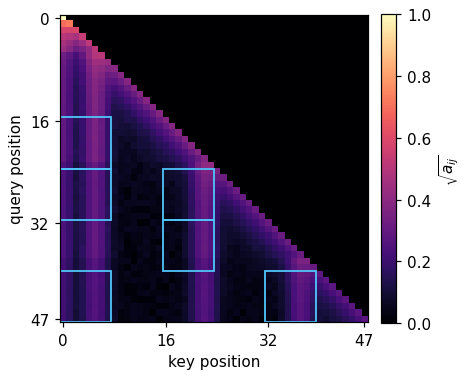
\includegraphics[width=0.8\linewidth]{figures/attention.png}
  \caption{Dense attention weights for one head of layer 18 on a 4k-token
  excerpt. Blocks selected by \textsc{Sieve} are outlined.}
  \label{fig:attention}
\end{figure}

\subsection{Ablations}

Removing the spread term $\sigma_i$ from the block score costs 2.1 points on
needle retrieval, and disabling selection reuse across layers increases
latency by 18\% with no change in accuracy. See \autoref{sec:analysis} for
why the spread term matters.

\section{Results}
\label{sec:results}

We evaluate on four long-context benchmarks: needle retrieval, multi-document
question answering, code completion over whole repositories, and long-form
summarisation. All models are 7B-parameter decoders fine-tuned at 32k tokens
and evaluated at up to 128k.

\begin{table}[ht]
  \centering
  \caption{Accuracy and keys read per query at 128k tokens. Higher accuracy is
  better; fewer keys is cheaper. Best sparse result in bold.}
  \label{tab:results}
  \begin{tabular}{lrrrr}
    \toprule
    Method        & Needle & Multi-doc QA & Repo code & Keys read \\
    \midrule
    Dense         & 99.1   & 71.4         & 58.2      & 131{,}072 \\
    Sliding window & 41.7  & 52.9         & 44.0      & 4{,}096   \\
    BigBird       & 88.3   & 63.0         & 51.6      & 12{,}288  \\
    Routing       & 95.6   & 68.1         & 55.9      & 16{,}384  \\
    \midrule
    \textsc{Sieve} ($k=8$)  & 97.8 & 69.9 & 56.7 & 6{,}144 \\
    \textsc{Sieve} ($k=16$) & \textbf{98.9} & \textbf{71.0} & \textbf{57.8} & 11{,}264 \\
    \bottomrule
  \end{tabular}
\end{table}

Table~\ref{tab:results} summarises the main comparison. \textsc{Sieve} with
$k = 16$ is within 0.4 points of dense attention on every task while reading
$11.6\times$ fewer keys. Sliding-window attention fails at needle retrieval,
as expected, because the answer is rarely local to the question.

\begin{figure}[ht]
  \centering
  %% Creator: Matplotlib, PGF backend
%%
%% To include the figure in your LaTeX document, write
%%   \input{<filename>.pgf}
%%
%% Make sure the required packages are loaded in your preamble
%%   \usepackage{pgf}
%%
%% Also ensure that all the required font packages are loaded; for instance,
%% the lmodern package is sometimes necessary when using math font.
%%   \usepackage{lmodern}
%%
%% Figures using additional raster images can only be included by \input if
%% they are in the same directory as the main LaTeX file. For loading figures
%% from other directories you can use the `import` package
%%   \usepackage{import}
%%
%% and then include the figures with
%%   \import{<path to file>}{<filename>.pgf}
%%
%% Matplotlib used the following preamble
%%   \def\mathdefault#1{#1}
%%   \everymath=\expandafter{\the\everymath\displaystyle}
%%   
%%   \ifdefined\pdftexversion\else  % non-pdftex case.
%%     \usepackage{fontspec}
%%     \setmainfont{DejaVuSerif.ttf}[Path=\detokenize{/Library/Frameworks/Python.framework/Versions/3.12/lib/python3.12/site-packages/matplotlib/mpl-data/fonts/ttf/}]
%%     \setsansfont{DejaVuSans.ttf}[Path=\detokenize{/Library/Frameworks/Python.framework/Versions/3.12/lib/python3.12/site-packages/matplotlib/mpl-data/fonts/ttf/}]
%%     \setmonofont{DejaVuSansMono.ttf}[Path=\detokenize{/Library/Frameworks/Python.framework/Versions/3.12/lib/python3.12/site-packages/matplotlib/mpl-data/fonts/ttf/}]
%%   \fi
%%   \makeatletter\@ifpackageloaded{underscore}{}{\usepackage[strings]{underscore}}\makeatother
%%
\begingroup%
\makeatletter%
\begin{pgfpicture}%
\pgfpathrectangle{\pgfpointorigin}{\pgfqpoint{4.600000in}{2.900000in}}%
\pgfusepath{use as bounding box, clip}%
\begin{pgfscope}%
\pgfsetbuttcap%
\pgfsetmiterjoin%
\definecolor{currentfill}{rgb}{1.000000,1.000000,1.000000}%
\pgfsetfillcolor{currentfill}%
\pgfsetlinewidth{0.000000pt}%
\definecolor{currentstroke}{rgb}{1.000000,1.000000,1.000000}%
\pgfsetstrokecolor{currentstroke}%
\pgfsetdash{}{0pt}%
\pgfpathmoveto{\pgfqpoint{0.000000in}{0.000000in}}%
\pgfpathlineto{\pgfqpoint{4.600000in}{0.000000in}}%
\pgfpathlineto{\pgfqpoint{4.600000in}{2.900000in}}%
\pgfpathlineto{\pgfqpoint{0.000000in}{2.900000in}}%
\pgfpathlineto{\pgfqpoint{0.000000in}{0.000000in}}%
\pgfpathclose%
\pgfusepath{fill}%
\end{pgfscope}%
\begin{pgfscope}%
\pgfsetbuttcap%
\pgfsetmiterjoin%
\definecolor{currentfill}{rgb}{1.000000,1.000000,1.000000}%
\pgfsetfillcolor{currentfill}%
\pgfsetlinewidth{0.000000pt}%
\definecolor{currentstroke}{rgb}{0.000000,0.000000,0.000000}%
\pgfsetstrokecolor{currentstroke}%
\pgfsetstrokeopacity{0.000000}%
\pgfsetdash{}{0pt}%
\pgfpathmoveto{\pgfqpoint{0.942108in}{0.582778in}}%
\pgfpathlineto{\pgfqpoint{4.450000in}{0.582778in}}%
\pgfpathlineto{\pgfqpoint{4.450000in}{2.750000in}}%
\pgfpathlineto{\pgfqpoint{0.942108in}{2.750000in}}%
\pgfpathlineto{\pgfqpoint{0.942108in}{0.582778in}}%
\pgfpathclose%
\pgfusepath{fill}%
\end{pgfscope}%
\begin{pgfscope}%
\pgfpathrectangle{\pgfqpoint{0.942108in}{0.582778in}}{\pgfqpoint{3.507892in}{2.167222in}}%
\pgfusepath{clip}%
\pgfsetbuttcap%
\pgfsetroundjoin%
\definecolor{currentfill}{rgb}{1.000000,0.584314,0.000000}%
\pgfsetfillcolor{currentfill}%
\pgfsetfillopacity{0.180000}%
\pgfsetlinewidth{0.000000pt}%
\definecolor{currentstroke}{rgb}{1.000000,0.584314,0.000000}%
\pgfsetstrokecolor{currentstroke}%
\pgfsetstrokeopacity{0.180000}%
\pgfsetdash{}{0pt}%
\pgfsys@defobject{currentmarker}{\pgfqpoint{1.101557in}{0.700885in}}{\pgfqpoint{4.290550in}{2.495498in}}{%
\pgfpathmoveto{\pgfqpoint{1.101557in}{2.495498in}}%
\pgfpathlineto{\pgfqpoint{1.101557in}{2.417550in}}%
\pgfpathlineto{\pgfqpoint{1.121488in}{2.374273in}}%
\pgfpathlineto{\pgfqpoint{1.141420in}{2.310227in}}%
\pgfpathlineto{\pgfqpoint{1.161351in}{2.287531in}}%
\pgfpathlineto{\pgfqpoint{1.181282in}{2.240011in}}%
\pgfpathlineto{\pgfqpoint{1.201213in}{2.215017in}}%
\pgfpathlineto{\pgfqpoint{1.221144in}{2.162805in}}%
\pgfpathlineto{\pgfqpoint{1.241076in}{2.119581in}}%
\pgfpathlineto{\pgfqpoint{1.261007in}{2.085505in}}%
\pgfpathlineto{\pgfqpoint{1.280938in}{2.050904in}}%
\pgfpathlineto{\pgfqpoint{1.300869in}{2.008160in}}%
\pgfpathlineto{\pgfqpoint{1.320800in}{1.976095in}}%
\pgfpathlineto{\pgfqpoint{1.340732in}{1.929877in}}%
\pgfpathlineto{\pgfqpoint{1.360663in}{1.904543in}}%
\pgfpathlineto{\pgfqpoint{1.380594in}{1.879047in}}%
\pgfpathlineto{\pgfqpoint{1.400525in}{1.856081in}}%
\pgfpathlineto{\pgfqpoint{1.420457in}{1.812893in}}%
\pgfpathlineto{\pgfqpoint{1.440388in}{1.777388in}}%
\pgfpathlineto{\pgfqpoint{1.460319in}{1.754407in}}%
\pgfpathlineto{\pgfqpoint{1.480250in}{1.722701in}}%
\pgfpathlineto{\pgfqpoint{1.500181in}{1.698938in}}%
\pgfpathlineto{\pgfqpoint{1.520113in}{1.664865in}}%
\pgfpathlineto{\pgfqpoint{1.540044in}{1.625673in}}%
\pgfpathlineto{\pgfqpoint{1.559975in}{1.601581in}}%
\pgfpathlineto{\pgfqpoint{1.579906in}{1.573959in}}%
\pgfpathlineto{\pgfqpoint{1.599837in}{1.548897in}}%
\pgfpathlineto{\pgfqpoint{1.619769in}{1.522375in}}%
\pgfpathlineto{\pgfqpoint{1.639700in}{1.488027in}}%
\pgfpathlineto{\pgfqpoint{1.659631in}{1.450840in}}%
\pgfpathlineto{\pgfqpoint{1.679562in}{1.441056in}}%
\pgfpathlineto{\pgfqpoint{1.699493in}{1.404633in}}%
\pgfpathlineto{\pgfqpoint{1.719425in}{1.402809in}}%
\pgfpathlineto{\pgfqpoint{1.739356in}{1.380364in}}%
\pgfpathlineto{\pgfqpoint{1.759287in}{1.342313in}}%
\pgfpathlineto{\pgfqpoint{1.779218in}{1.345331in}}%
\pgfpathlineto{\pgfqpoint{1.799149in}{1.327086in}}%
\pgfpathlineto{\pgfqpoint{1.819081in}{1.299820in}}%
\pgfpathlineto{\pgfqpoint{1.839012in}{1.296794in}}%
\pgfpathlineto{\pgfqpoint{1.858943in}{1.280513in}}%
\pgfpathlineto{\pgfqpoint{1.878874in}{1.231137in}}%
\pgfpathlineto{\pgfqpoint{1.898805in}{1.236844in}}%
\pgfpathlineto{\pgfqpoint{1.918737in}{1.213867in}}%
\pgfpathlineto{\pgfqpoint{1.938668in}{1.197274in}}%
\pgfpathlineto{\pgfqpoint{1.958599in}{1.186760in}}%
\pgfpathlineto{\pgfqpoint{1.978530in}{1.154095in}}%
\pgfpathlineto{\pgfqpoint{1.998462in}{1.140456in}}%
\pgfpathlineto{\pgfqpoint{2.018393in}{1.123469in}}%
\pgfpathlineto{\pgfqpoint{2.038324in}{1.110151in}}%
\pgfpathlineto{\pgfqpoint{2.058255in}{1.103458in}}%
\pgfpathlineto{\pgfqpoint{2.078186in}{1.075874in}}%
\pgfpathlineto{\pgfqpoint{2.098118in}{1.067387in}}%
\pgfpathlineto{\pgfqpoint{2.118049in}{1.072241in}}%
\pgfpathlineto{\pgfqpoint{2.137980in}{1.053360in}}%
\pgfpathlineto{\pgfqpoint{2.157911in}{1.046571in}}%
\pgfpathlineto{\pgfqpoint{2.177842in}{1.011003in}}%
\pgfpathlineto{\pgfqpoint{2.197774in}{1.011974in}}%
\pgfpathlineto{\pgfqpoint{2.217705in}{1.003878in}}%
\pgfpathlineto{\pgfqpoint{2.237636in}{0.999971in}}%
\pgfpathlineto{\pgfqpoint{2.257567in}{0.983480in}}%
\pgfpathlineto{\pgfqpoint{2.277498in}{0.990178in}}%
\pgfpathlineto{\pgfqpoint{2.297430in}{0.970365in}}%
\pgfpathlineto{\pgfqpoint{2.317361in}{0.962247in}}%
\pgfpathlineto{\pgfqpoint{2.337292in}{0.953582in}}%
\pgfpathlineto{\pgfqpoint{2.357223in}{0.952656in}}%
\pgfpathlineto{\pgfqpoint{2.377154in}{0.931985in}}%
\pgfpathlineto{\pgfqpoint{2.397086in}{0.941206in}}%
\pgfpathlineto{\pgfqpoint{2.417017in}{0.926623in}}%
\pgfpathlineto{\pgfqpoint{2.436948in}{0.916085in}}%
\pgfpathlineto{\pgfqpoint{2.456879in}{0.907859in}}%
\pgfpathlineto{\pgfqpoint{2.476810in}{0.906163in}}%
\pgfpathlineto{\pgfqpoint{2.496742in}{0.904850in}}%
\pgfpathlineto{\pgfqpoint{2.516673in}{0.897768in}}%
\pgfpathlineto{\pgfqpoint{2.536604in}{0.885615in}}%
\pgfpathlineto{\pgfqpoint{2.556535in}{0.885001in}}%
\pgfpathlineto{\pgfqpoint{2.576467in}{0.871282in}}%
\pgfpathlineto{\pgfqpoint{2.596398in}{0.877727in}}%
\pgfpathlineto{\pgfqpoint{2.616329in}{0.858941in}}%
\pgfpathlineto{\pgfqpoint{2.636260in}{0.832128in}}%
\pgfpathlineto{\pgfqpoint{2.656191in}{0.863177in}}%
\pgfpathlineto{\pgfqpoint{2.676123in}{0.845518in}}%
\pgfpathlineto{\pgfqpoint{2.696054in}{0.827485in}}%
\pgfpathlineto{\pgfqpoint{2.715985in}{0.833274in}}%
\pgfpathlineto{\pgfqpoint{2.735916in}{0.821827in}}%
\pgfpathlineto{\pgfqpoint{2.755847in}{0.848677in}}%
\pgfpathlineto{\pgfqpoint{2.775779in}{0.828111in}}%
\pgfpathlineto{\pgfqpoint{2.795710in}{0.802798in}}%
\pgfpathlineto{\pgfqpoint{2.815641in}{0.821040in}}%
\pgfpathlineto{\pgfqpoint{2.835572in}{0.807719in}}%
\pgfpathlineto{\pgfqpoint{2.855503in}{0.828004in}}%
\pgfpathlineto{\pgfqpoint{2.875435in}{0.794247in}}%
\pgfpathlineto{\pgfqpoint{2.895366in}{0.778763in}}%
\pgfpathlineto{\pgfqpoint{2.915297in}{0.799455in}}%
\pgfpathlineto{\pgfqpoint{2.935228in}{0.792266in}}%
\pgfpathlineto{\pgfqpoint{2.955159in}{0.788714in}}%
\pgfpathlineto{\pgfqpoint{2.975091in}{0.768414in}}%
\pgfpathlineto{\pgfqpoint{2.995022in}{0.791818in}}%
\pgfpathlineto{\pgfqpoint{3.014953in}{0.801711in}}%
\pgfpathlineto{\pgfqpoint{3.034884in}{0.763259in}}%
\pgfpathlineto{\pgfqpoint{3.054815in}{0.791773in}}%
\pgfpathlineto{\pgfqpoint{3.074747in}{0.772132in}}%
\pgfpathlineto{\pgfqpoint{3.094678in}{0.798798in}}%
\pgfpathlineto{\pgfqpoint{3.114609in}{0.777778in}}%
\pgfpathlineto{\pgfqpoint{3.134540in}{0.769560in}}%
\pgfpathlineto{\pgfqpoint{3.154472in}{0.780285in}}%
\pgfpathlineto{\pgfqpoint{3.174403in}{0.772687in}}%
\pgfpathlineto{\pgfqpoint{3.194334in}{0.759906in}}%
\pgfpathlineto{\pgfqpoint{3.214265in}{0.770844in}}%
\pgfpathlineto{\pgfqpoint{3.234196in}{0.757275in}}%
\pgfpathlineto{\pgfqpoint{3.254128in}{0.743228in}}%
\pgfpathlineto{\pgfqpoint{3.274059in}{0.778522in}}%
\pgfpathlineto{\pgfqpoint{3.293990in}{0.754145in}}%
\pgfpathlineto{\pgfqpoint{3.313921in}{0.750206in}}%
\pgfpathlineto{\pgfqpoint{3.333852in}{0.757868in}}%
\pgfpathlineto{\pgfqpoint{3.353784in}{0.738404in}}%
\pgfpathlineto{\pgfqpoint{3.373715in}{0.739117in}}%
\pgfpathlineto{\pgfqpoint{3.393646in}{0.746003in}}%
\pgfpathlineto{\pgfqpoint{3.413577in}{0.744622in}}%
\pgfpathlineto{\pgfqpoint{3.433508in}{0.749027in}}%
\pgfpathlineto{\pgfqpoint{3.453440in}{0.757690in}}%
\pgfpathlineto{\pgfqpoint{3.473371in}{0.741741in}}%
\pgfpathlineto{\pgfqpoint{3.493302in}{0.749682in}}%
\pgfpathlineto{\pgfqpoint{3.513233in}{0.749669in}}%
\pgfpathlineto{\pgfqpoint{3.533164in}{0.733162in}}%
\pgfpathlineto{\pgfqpoint{3.553096in}{0.744330in}}%
\pgfpathlineto{\pgfqpoint{3.573027in}{0.732720in}}%
\pgfpathlineto{\pgfqpoint{3.592958in}{0.750149in}}%
\pgfpathlineto{\pgfqpoint{3.612889in}{0.743789in}}%
\pgfpathlineto{\pgfqpoint{3.632821in}{0.739025in}}%
\pgfpathlineto{\pgfqpoint{3.652752in}{0.726028in}}%
\pgfpathlineto{\pgfqpoint{3.672683in}{0.738420in}}%
\pgfpathlineto{\pgfqpoint{3.692614in}{0.729817in}}%
\pgfpathlineto{\pgfqpoint{3.712545in}{0.742266in}}%
\pgfpathlineto{\pgfqpoint{3.732477in}{0.734287in}}%
\pgfpathlineto{\pgfqpoint{3.752408in}{0.727536in}}%
\pgfpathlineto{\pgfqpoint{3.772339in}{0.742233in}}%
\pgfpathlineto{\pgfqpoint{3.792270in}{0.739840in}}%
\pgfpathlineto{\pgfqpoint{3.812201in}{0.727793in}}%
\pgfpathlineto{\pgfqpoint{3.832133in}{0.742508in}}%
\pgfpathlineto{\pgfqpoint{3.852064in}{0.729337in}}%
\pgfpathlineto{\pgfqpoint{3.871995in}{0.728757in}}%
\pgfpathlineto{\pgfqpoint{3.891926in}{0.732009in}}%
\pgfpathlineto{\pgfqpoint{3.911857in}{0.724041in}}%
\pgfpathlineto{\pgfqpoint{3.931789in}{0.726280in}}%
\pgfpathlineto{\pgfqpoint{3.951720in}{0.728259in}}%
\pgfpathlineto{\pgfqpoint{3.971651in}{0.742106in}}%
\pgfpathlineto{\pgfqpoint{3.991582in}{0.741407in}}%
\pgfpathlineto{\pgfqpoint{4.011513in}{0.726273in}}%
\pgfpathlineto{\pgfqpoint{4.031445in}{0.741487in}}%
\pgfpathlineto{\pgfqpoint{4.051376in}{0.727374in}}%
\pgfpathlineto{\pgfqpoint{4.071307in}{0.730549in}}%
\pgfpathlineto{\pgfqpoint{4.091238in}{0.734355in}}%
\pgfpathlineto{\pgfqpoint{4.111169in}{0.729167in}}%
\pgfpathlineto{\pgfqpoint{4.131101in}{0.746147in}}%
\pgfpathlineto{\pgfqpoint{4.151032in}{0.728169in}}%
\pgfpathlineto{\pgfqpoint{4.170963in}{0.716167in}}%
\pgfpathlineto{\pgfqpoint{4.190894in}{0.736178in}}%
\pgfpathlineto{\pgfqpoint{4.210826in}{0.722074in}}%
\pgfpathlineto{\pgfqpoint{4.230757in}{0.722710in}}%
\pgfpathlineto{\pgfqpoint{4.250688in}{0.700885in}}%
\pgfpathlineto{\pgfqpoint{4.270619in}{0.732643in}}%
\pgfpathlineto{\pgfqpoint{4.290550in}{0.730954in}}%
\pgfpathlineto{\pgfqpoint{4.290550in}{0.799688in}}%
\pgfpathlineto{\pgfqpoint{4.290550in}{0.799688in}}%
\pgfpathlineto{\pgfqpoint{4.270619in}{0.801403in}}%
\pgfpathlineto{\pgfqpoint{4.250688in}{0.770748in}}%
\pgfpathlineto{\pgfqpoint{4.230757in}{0.791953in}}%
\pgfpathlineto{\pgfqpoint{4.210826in}{0.791423in}}%
\pgfpathlineto{\pgfqpoint{4.190894in}{0.805161in}}%
\pgfpathlineto{\pgfqpoint{4.170963in}{0.785882in}}%
\pgfpathlineto{\pgfqpoint{4.151032in}{0.797588in}}%
\pgfpathlineto{\pgfqpoint{4.131101in}{0.815081in}}%
\pgfpathlineto{\pgfqpoint{4.111169in}{0.798741in}}%
\pgfpathlineto{\pgfqpoint{4.091238in}{0.803858in}}%
\pgfpathlineto{\pgfqpoint{4.071307in}{0.800274in}}%
\pgfpathlineto{\pgfqpoint{4.051376in}{0.797302in}}%
\pgfpathlineto{\pgfqpoint{4.031445in}{0.811061in}}%
\pgfpathlineto{\pgfqpoint{4.011513in}{0.796444in}}%
\pgfpathlineto{\pgfqpoint{3.991582in}{0.811194in}}%
\pgfpathlineto{\pgfqpoint{3.971651in}{0.811979in}}%
\pgfpathlineto{\pgfqpoint{3.951720in}{0.798694in}}%
\pgfpathlineto{\pgfqpoint{3.931789in}{0.796894in}}%
\pgfpathlineto{\pgfqpoint{3.911857in}{0.794844in}}%
\pgfpathlineto{\pgfqpoint{3.891926in}{0.802669in}}%
\pgfpathlineto{\pgfqpoint{3.871995in}{0.799645in}}%
\pgfpathlineto{\pgfqpoint{3.852064in}{0.800329in}}%
\pgfpathlineto{\pgfqpoint{3.832133in}{0.813194in}}%
\pgfpathlineto{\pgfqpoint{3.812201in}{0.799092in}}%
\pgfpathlineto{\pgfqpoint{3.792270in}{0.810874in}}%
\pgfpathlineto{\pgfqpoint{3.772339in}{0.813321in}}%
\pgfpathlineto{\pgfqpoint{3.752408in}{0.799247in}}%
\pgfpathlineto{\pgfqpoint{3.732477in}{0.805914in}}%
\pgfpathlineto{\pgfqpoint{3.712545in}{0.813771in}}%
\pgfpathlineto{\pgfqpoint{3.692614in}{0.801882in}}%
\pgfpathlineto{\pgfqpoint{3.672683in}{0.810346in}}%
\pgfpathlineto{\pgfqpoint{3.652752in}{0.798521in}}%
\pgfpathlineto{\pgfqpoint{3.632821in}{0.811238in}}%
\pgfpathlineto{\pgfqpoint{3.612889in}{0.816000in}}%
\pgfpathlineto{\pgfqpoint{3.592958in}{0.822308in}}%
\pgfpathlineto{\pgfqpoint{3.573027in}{0.805630in}}%
\pgfpathlineto{\pgfqpoint{3.553096in}{0.817016in}}%
\pgfpathlineto{\pgfqpoint{3.533164in}{0.806398in}}%
\pgfpathlineto{\pgfqpoint{3.513233in}{0.822521in}}%
\pgfpathlineto{\pgfqpoint{3.493302in}{0.822712in}}%
\pgfpathlineto{\pgfqpoint{3.473371in}{0.815222in}}%
\pgfpathlineto{\pgfqpoint{3.453440in}{0.830816in}}%
\pgfpathlineto{\pgfqpoint{3.433508in}{0.822636in}}%
\pgfpathlineto{\pgfqpoint{3.413577in}{0.818575in}}%
\pgfpathlineto{\pgfqpoint{3.393646in}{0.820107in}}%
\pgfpathlineto{\pgfqpoint{3.373715in}{0.813661in}}%
\pgfpathlineto{\pgfqpoint{3.353784in}{0.813179in}}%
\pgfpathlineto{\pgfqpoint{3.333852in}{0.832181in}}%
\pgfpathlineto{\pgfqpoint{3.313921in}{0.824999in}}%
\pgfpathlineto{\pgfqpoint{3.293990in}{0.829020in}}%
\pgfpathlineto{\pgfqpoint{3.274059in}{0.852777in}}%
\pgfpathlineto{\pgfqpoint{3.254128in}{0.818936in}}%
\pgfpathlineto{\pgfqpoint{3.234196in}{0.832724in}}%
\pgfpathlineto{\pgfqpoint{3.214265in}{0.846057in}}%
\pgfpathlineto{\pgfqpoint{3.194334in}{0.835742in}}%
\pgfpathlineto{\pgfqpoint{3.174403in}{0.848322in}}%
\pgfpathlineto{\pgfqpoint{3.154472in}{0.855904in}}%
\pgfpathlineto{\pgfqpoint{3.134540in}{0.845812in}}%
\pgfpathlineto{\pgfqpoint{3.114609in}{0.854001in}}%
\pgfpathlineto{\pgfqpoint{3.094678in}{0.874546in}}%
\pgfpathlineto{\pgfqpoint{3.074747in}{0.849094in}}%
\pgfpathlineto{\pgfqpoint{3.054815in}{0.868314in}}%
\pgfpathlineto{\pgfqpoint{3.034884in}{0.841102in}}%
\pgfpathlineto{\pgfqpoint{3.014953in}{0.878467in}}%
\pgfpathlineto{\pgfqpoint{2.995022in}{0.869220in}}%
\pgfpathlineto{\pgfqpoint{2.975091in}{0.846961in}}%
\pgfpathlineto{\pgfqpoint{2.955159in}{0.866832in}}%
\pgfpathlineto{\pgfqpoint{2.935228in}{0.870569in}}%
\pgfpathlineto{\pgfqpoint{2.915297in}{0.877815in}}%
\pgfpathlineto{\pgfqpoint{2.895366in}{0.858204in}}%
\pgfpathlineto{\pgfqpoint{2.875435in}{0.873453in}}%
\pgfpathlineto{\pgfqpoint{2.855503in}{0.906316in}}%
\pgfpathlineto{\pgfqpoint{2.835572in}{0.887113in}}%
\pgfpathlineto{\pgfqpoint{2.815641in}{0.900295in}}%
\pgfpathlineto{\pgfqpoint{2.795710in}{0.883084in}}%
\pgfpathlineto{\pgfqpoint{2.775779in}{0.907824in}}%
\pgfpathlineto{\pgfqpoint{2.755847in}{0.928001in}}%
\pgfpathlineto{\pgfqpoint{2.735916in}{0.902521in}}%
\pgfpathlineto{\pgfqpoint{2.715985in}{0.913927in}}%
\pgfpathlineto{\pgfqpoint{2.696054in}{0.908748in}}%
\pgfpathlineto{\pgfqpoint{2.676123in}{0.926505in}}%
\pgfpathlineto{\pgfqpoint{2.656191in}{0.943908in}}%
\pgfpathlineto{\pgfqpoint{2.636260in}{0.914444in}}%
\pgfpathlineto{\pgfqpoint{2.616329in}{0.940665in}}%
\pgfpathlineto{\pgfqpoint{2.596398in}{0.959170in}}%
\pgfpathlineto{\pgfqpoint{2.576467in}{0.953405in}}%
\pgfpathlineto{\pgfqpoint{2.556535in}{0.967048in}}%
\pgfpathlineto{\pgfqpoint{2.536604in}{0.968090in}}%
\pgfpathlineto{\pgfqpoint{2.516673in}{0.980241in}}%
\pgfpathlineto{\pgfqpoint{2.496742in}{0.987521in}}%
\pgfpathlineto{\pgfqpoint{2.476810in}{0.989259in}}%
\pgfpathlineto{\pgfqpoint{2.456879in}{0.991377in}}%
\pgfpathlineto{\pgfqpoint{2.436948in}{0.999779in}}%
\pgfpathlineto{\pgfqpoint{2.417017in}{1.010414in}}%
\pgfpathlineto{\pgfqpoint{2.397086in}{1.024943in}}%
\pgfpathlineto{\pgfqpoint{2.377154in}{1.016602in}}%
\pgfpathlineto{\pgfqpoint{2.357223in}{1.036996in}}%
\pgfpathlineto{\pgfqpoint{2.337292in}{1.038425in}}%
\pgfpathlineto{\pgfqpoint{2.317361in}{1.047298in}}%
\pgfpathlineto{\pgfqpoint{2.297430in}{1.055655in}}%
\pgfpathlineto{\pgfqpoint{2.277498in}{1.075254in}}%
\pgfpathlineto{\pgfqpoint{2.257567in}{1.069397in}}%
\pgfpathlineto{\pgfqpoint{2.237636in}{1.085821in}}%
\pgfpathlineto{\pgfqpoint{2.217705in}{1.090169in}}%
\pgfpathlineto{\pgfqpoint{2.197774in}{1.098549in}}%
\pgfpathlineto{\pgfqpoint{2.177842in}{1.098235in}}%
\pgfpathlineto{\pgfqpoint{2.157911in}{1.133003in}}%
\pgfpathlineto{\pgfqpoint{2.137980in}{1.140154in}}%
\pgfpathlineto{\pgfqpoint{2.118049in}{1.158921in}}%
\pgfpathlineto{\pgfqpoint{2.098118in}{1.154917in}}%
\pgfpathlineto{\pgfqpoint{2.078186in}{1.163727in}}%
\pgfpathlineto{\pgfqpoint{2.058255in}{1.190870in}}%
\pgfpathlineto{\pgfqpoint{2.038324in}{1.197977in}}%
\pgfpathlineto{\pgfqpoint{2.018393in}{1.211449in}}%
\pgfpathlineto{\pgfqpoint{1.998462in}{1.228450in}}%
\pgfpathlineto{\pgfqpoint{1.978530in}{1.242249in}}%
\pgfpathlineto{\pgfqpoint{1.958599in}{1.274310in}}%
\pgfpathlineto{\pgfqpoint{1.938668in}{1.285127in}}%
\pgfpathlineto{\pgfqpoint{1.918737in}{1.301787in}}%
\pgfpathlineto{\pgfqpoint{1.898805in}{1.324581in}}%
\pgfpathlineto{\pgfqpoint{1.878874in}{1.319867in}}%
\pgfpathlineto{\pgfqpoint{1.858943in}{1.368003in}}%
\pgfpathlineto{\pgfqpoint{1.839012in}{1.384399in}}%
\pgfpathlineto{\pgfqpoint{1.819081in}{1.388088in}}%
\pgfpathlineto{\pgfqpoint{1.799149in}{1.415041in}}%
\pgfpathlineto{\pgfqpoint{1.779218in}{1.433350in}}%
\pgfpathlineto{\pgfqpoint{1.759287in}{1.431274in}}%
\pgfpathlineto{\pgfqpoint{1.739356in}{1.468597in}}%
\pgfpathlineto{\pgfqpoint{1.719425in}{1.490963in}}%
\pgfpathlineto{\pgfqpoint{1.699493in}{1.493559in}}%
\pgfpathlineto{\pgfqpoint{1.679562in}{1.529349in}}%
\pgfpathlineto{\pgfqpoint{1.659631in}{1.539599in}}%
\pgfpathlineto{\pgfqpoint{1.639700in}{1.576142in}}%
\pgfpathlineto{\pgfqpoint{1.619769in}{1.609975in}}%
\pgfpathlineto{\pgfqpoint{1.599837in}{1.636309in}}%
\pgfpathlineto{\pgfqpoint{1.579906in}{1.661251in}}%
\pgfpathlineto{\pgfqpoint{1.559975in}{1.688660in}}%
\pgfpathlineto{\pgfqpoint{1.540044in}{1.712691in}}%
\pgfpathlineto{\pgfqpoint{1.520113in}{1.751226in}}%
\pgfpathlineto{\pgfqpoint{1.500181in}{1.784859in}}%
\pgfpathlineto{\pgfqpoint{1.480250in}{1.808602in}}%
\pgfpathlineto{\pgfqpoint{1.460319in}{1.839982in}}%
\pgfpathlineto{\pgfqpoint{1.440388in}{1.862992in}}%
\pgfpathlineto{\pgfqpoint{1.420457in}{1.898040in}}%
\pgfpathlineto{\pgfqpoint{1.400525in}{1.940483in}}%
\pgfpathlineto{\pgfqpoint{1.380594in}{1.963505in}}%
\pgfpathlineto{\pgfqpoint{1.360663in}{1.988967in}}%
\pgfpathlineto{\pgfqpoint{1.340732in}{2.014282in}}%
\pgfpathlineto{\pgfqpoint{1.320800in}{2.059679in}}%
\pgfpathlineto{\pgfqpoint{1.300869in}{2.091484in}}%
\pgfpathlineto{\pgfqpoint{1.280938in}{2.133567in}}%
\pgfpathlineto{\pgfqpoint{1.261007in}{2.167830in}}%
\pgfpathlineto{\pgfqpoint{1.241076in}{2.201598in}}%
\pgfpathlineto{\pgfqpoint{1.221144in}{2.244179in}}%
\pgfpathlineto{\pgfqpoint{1.201213in}{2.295425in}}%
\pgfpathlineto{\pgfqpoint{1.181282in}{2.320481in}}%
\pgfpathlineto{\pgfqpoint{1.161351in}{2.367236in}}%
\pgfpathlineto{\pgfqpoint{1.141420in}{2.390093in}}%
\pgfpathlineto{\pgfqpoint{1.121488in}{2.452793in}}%
\pgfpathlineto{\pgfqpoint{1.101557in}{2.495498in}}%
\pgfpathlineto{\pgfqpoint{1.101557in}{2.495498in}}%
\pgfpathclose%
\pgfusepath{fill}%
}%
\begin{pgfscope}%
\pgfsys@transformshift{0.000000in}{0.000000in}%
\pgfsys@useobject{currentmarker}{}%
\end{pgfscope}%
\end{pgfscope}%
\begin{pgfscope}%
\pgfpathrectangle{\pgfqpoint{0.942108in}{0.582778in}}{\pgfqpoint{3.507892in}{2.167222in}}%
\pgfusepath{clip}%
\pgfsetrectcap%
\pgfsetroundjoin%
\pgfsetlinewidth{0.602250pt}%
\definecolor{currentstroke}{rgb}{0.819608,0.819608,0.839216}%
\pgfsetstrokecolor{currentstroke}%
\pgfsetdash{}{0pt}%
\pgfpathmoveto{\pgfqpoint{1.101557in}{0.582778in}}%
\pgfpathlineto{\pgfqpoint{1.101557in}{2.750000in}}%
\pgfusepath{stroke}%
\end{pgfscope}%
\begin{pgfscope}%
\pgfsetbuttcap%
\pgfsetroundjoin%
\definecolor{currentfill}{rgb}{0.000000,0.000000,0.000000}%
\pgfsetfillcolor{currentfill}%
\pgfsetlinewidth{0.803000pt}%
\definecolor{currentstroke}{rgb}{0.000000,0.000000,0.000000}%
\pgfsetstrokecolor{currentstroke}%
\pgfsetdash{}{0pt}%
\pgfsys@defobject{currentmarker}{\pgfqpoint{0.000000in}{-0.048611in}}{\pgfqpoint{0.000000in}{0.000000in}}{%
\pgfpathmoveto{\pgfqpoint{0.000000in}{0.000000in}}%
\pgfpathlineto{\pgfqpoint{0.000000in}{-0.048611in}}%
\pgfusepath{stroke,fill}%
}%
\begin{pgfscope}%
\pgfsys@transformshift{1.101557in}{0.582778in}%
\pgfsys@useobject{currentmarker}{}%
\end{pgfscope}%
\end{pgfscope}%
\begin{pgfscope}%
\definecolor{textcolor}{rgb}{0.000000,0.000000,0.000000}%
\pgfsetstrokecolor{textcolor}%
\pgfsetfillcolor{textcolor}%
\pgftext[x=1.101557in,y=0.485556in,,top]{\color{textcolor}{\sffamily\fontsize{10.000000}{12.000000}\selectfont\catcode`\^=\active\def^{\ifmmode\sp\else\^{}\fi}\catcode`\%=\active\def%{\%}0}}%
\end{pgfscope}%
\begin{pgfscope}%
\pgfpathrectangle{\pgfqpoint{0.942108in}{0.582778in}}{\pgfqpoint{3.507892in}{2.167222in}}%
\pgfusepath{clip}%
\pgfsetrectcap%
\pgfsetroundjoin%
\pgfsetlinewidth{0.602250pt}%
\definecolor{currentstroke}{rgb}{0.819608,0.819608,0.839216}%
\pgfsetstrokecolor{currentstroke}%
\pgfsetdash{}{0pt}%
\pgfpathmoveto{\pgfqpoint{1.898805in}{0.582778in}}%
\pgfpathlineto{\pgfqpoint{1.898805in}{2.750000in}}%
\pgfusepath{stroke}%
\end{pgfscope}%
\begin{pgfscope}%
\pgfsetbuttcap%
\pgfsetroundjoin%
\definecolor{currentfill}{rgb}{0.000000,0.000000,0.000000}%
\pgfsetfillcolor{currentfill}%
\pgfsetlinewidth{0.803000pt}%
\definecolor{currentstroke}{rgb}{0.000000,0.000000,0.000000}%
\pgfsetstrokecolor{currentstroke}%
\pgfsetdash{}{0pt}%
\pgfsys@defobject{currentmarker}{\pgfqpoint{0.000000in}{-0.048611in}}{\pgfqpoint{0.000000in}{0.000000in}}{%
\pgfpathmoveto{\pgfqpoint{0.000000in}{0.000000in}}%
\pgfpathlineto{\pgfqpoint{0.000000in}{-0.048611in}}%
\pgfusepath{stroke,fill}%
}%
\begin{pgfscope}%
\pgfsys@transformshift{1.898805in}{0.582778in}%
\pgfsys@useobject{currentmarker}{}%
\end{pgfscope}%
\end{pgfscope}%
\begin{pgfscope}%
\definecolor{textcolor}{rgb}{0.000000,0.000000,0.000000}%
\pgfsetstrokecolor{textcolor}%
\pgfsetfillcolor{textcolor}%
\pgftext[x=1.898805in,y=0.485556in,,top]{\color{textcolor}{\sffamily\fontsize{10.000000}{12.000000}\selectfont\catcode`\^=\active\def^{\ifmmode\sp\else\^{}\fi}\catcode`\%=\active\def%{\%}5k}}%
\end{pgfscope}%
\begin{pgfscope}%
\pgfpathrectangle{\pgfqpoint{0.942108in}{0.582778in}}{\pgfqpoint{3.507892in}{2.167222in}}%
\pgfusepath{clip}%
\pgfsetrectcap%
\pgfsetroundjoin%
\pgfsetlinewidth{0.602250pt}%
\definecolor{currentstroke}{rgb}{0.819608,0.819608,0.839216}%
\pgfsetstrokecolor{currentstroke}%
\pgfsetdash{}{0pt}%
\pgfpathmoveto{\pgfqpoint{2.696054in}{0.582778in}}%
\pgfpathlineto{\pgfqpoint{2.696054in}{2.750000in}}%
\pgfusepath{stroke}%
\end{pgfscope}%
\begin{pgfscope}%
\pgfsetbuttcap%
\pgfsetroundjoin%
\definecolor{currentfill}{rgb}{0.000000,0.000000,0.000000}%
\pgfsetfillcolor{currentfill}%
\pgfsetlinewidth{0.803000pt}%
\definecolor{currentstroke}{rgb}{0.000000,0.000000,0.000000}%
\pgfsetstrokecolor{currentstroke}%
\pgfsetdash{}{0pt}%
\pgfsys@defobject{currentmarker}{\pgfqpoint{0.000000in}{-0.048611in}}{\pgfqpoint{0.000000in}{0.000000in}}{%
\pgfpathmoveto{\pgfqpoint{0.000000in}{0.000000in}}%
\pgfpathlineto{\pgfqpoint{0.000000in}{-0.048611in}}%
\pgfusepath{stroke,fill}%
}%
\begin{pgfscope}%
\pgfsys@transformshift{2.696054in}{0.582778in}%
\pgfsys@useobject{currentmarker}{}%
\end{pgfscope}%
\end{pgfscope}%
\begin{pgfscope}%
\definecolor{textcolor}{rgb}{0.000000,0.000000,0.000000}%
\pgfsetstrokecolor{textcolor}%
\pgfsetfillcolor{textcolor}%
\pgftext[x=2.696054in,y=0.485556in,,top]{\color{textcolor}{\sffamily\fontsize{10.000000}{12.000000}\selectfont\catcode`\^=\active\def^{\ifmmode\sp\else\^{}\fi}\catcode`\%=\active\def%{\%}10k}}%
\end{pgfscope}%
\begin{pgfscope}%
\pgfpathrectangle{\pgfqpoint{0.942108in}{0.582778in}}{\pgfqpoint{3.507892in}{2.167222in}}%
\pgfusepath{clip}%
\pgfsetrectcap%
\pgfsetroundjoin%
\pgfsetlinewidth{0.602250pt}%
\definecolor{currentstroke}{rgb}{0.819608,0.819608,0.839216}%
\pgfsetstrokecolor{currentstroke}%
\pgfsetdash{}{0pt}%
\pgfpathmoveto{\pgfqpoint{3.493302in}{0.582778in}}%
\pgfpathlineto{\pgfqpoint{3.493302in}{2.750000in}}%
\pgfusepath{stroke}%
\end{pgfscope}%
\begin{pgfscope}%
\pgfsetbuttcap%
\pgfsetroundjoin%
\definecolor{currentfill}{rgb}{0.000000,0.000000,0.000000}%
\pgfsetfillcolor{currentfill}%
\pgfsetlinewidth{0.803000pt}%
\definecolor{currentstroke}{rgb}{0.000000,0.000000,0.000000}%
\pgfsetstrokecolor{currentstroke}%
\pgfsetdash{}{0pt}%
\pgfsys@defobject{currentmarker}{\pgfqpoint{0.000000in}{-0.048611in}}{\pgfqpoint{0.000000in}{0.000000in}}{%
\pgfpathmoveto{\pgfqpoint{0.000000in}{0.000000in}}%
\pgfpathlineto{\pgfqpoint{0.000000in}{-0.048611in}}%
\pgfusepath{stroke,fill}%
}%
\begin{pgfscope}%
\pgfsys@transformshift{3.493302in}{0.582778in}%
\pgfsys@useobject{currentmarker}{}%
\end{pgfscope}%
\end{pgfscope}%
\begin{pgfscope}%
\definecolor{textcolor}{rgb}{0.000000,0.000000,0.000000}%
\pgfsetstrokecolor{textcolor}%
\pgfsetfillcolor{textcolor}%
\pgftext[x=3.493302in,y=0.485556in,,top]{\color{textcolor}{\sffamily\fontsize{10.000000}{12.000000}\selectfont\catcode`\^=\active\def^{\ifmmode\sp\else\^{}\fi}\catcode`\%=\active\def%{\%}15k}}%
\end{pgfscope}%
\begin{pgfscope}%
\pgfpathrectangle{\pgfqpoint{0.942108in}{0.582778in}}{\pgfqpoint{3.507892in}{2.167222in}}%
\pgfusepath{clip}%
\pgfsetrectcap%
\pgfsetroundjoin%
\pgfsetlinewidth{0.602250pt}%
\definecolor{currentstroke}{rgb}{0.819608,0.819608,0.839216}%
\pgfsetstrokecolor{currentstroke}%
\pgfsetdash{}{0pt}%
\pgfpathmoveto{\pgfqpoint{4.290550in}{0.582778in}}%
\pgfpathlineto{\pgfqpoint{4.290550in}{2.750000in}}%
\pgfusepath{stroke}%
\end{pgfscope}%
\begin{pgfscope}%
\pgfsetbuttcap%
\pgfsetroundjoin%
\definecolor{currentfill}{rgb}{0.000000,0.000000,0.000000}%
\pgfsetfillcolor{currentfill}%
\pgfsetlinewidth{0.803000pt}%
\definecolor{currentstroke}{rgb}{0.000000,0.000000,0.000000}%
\pgfsetstrokecolor{currentstroke}%
\pgfsetdash{}{0pt}%
\pgfsys@defobject{currentmarker}{\pgfqpoint{0.000000in}{-0.048611in}}{\pgfqpoint{0.000000in}{0.000000in}}{%
\pgfpathmoveto{\pgfqpoint{0.000000in}{0.000000in}}%
\pgfpathlineto{\pgfqpoint{0.000000in}{-0.048611in}}%
\pgfusepath{stroke,fill}%
}%
\begin{pgfscope}%
\pgfsys@transformshift{4.290550in}{0.582778in}%
\pgfsys@useobject{currentmarker}{}%
\end{pgfscope}%
\end{pgfscope}%
\begin{pgfscope}%
\definecolor{textcolor}{rgb}{0.000000,0.000000,0.000000}%
\pgfsetstrokecolor{textcolor}%
\pgfsetfillcolor{textcolor}%
\pgftext[x=4.290550in,y=0.485556in,,top]{\color{textcolor}{\sffamily\fontsize{10.000000}{12.000000}\selectfont\catcode`\^=\active\def^{\ifmmode\sp\else\^{}\fi}\catcode`\%=\active\def%{\%}20k}}%
\end{pgfscope}%
\begin{pgfscope}%
\definecolor{textcolor}{rgb}{0.000000,0.000000,0.000000}%
\pgfsetstrokecolor{textcolor}%
\pgfsetfillcolor{textcolor}%
\pgftext[x=2.696054in,y=0.329200in,,top]{\color{textcolor}{\sffamily\fontsize{10.000000}{12.000000}\selectfont\catcode`\^=\active\def^{\ifmmode\sp\else\^{}\fi}\catcode`\%=\active\def%{\%}training step}}%
\end{pgfscope}%
\begin{pgfscope}%
\pgfsetbuttcap%
\pgfsetroundjoin%
\definecolor{currentfill}{rgb}{0.000000,0.000000,0.000000}%
\pgfsetfillcolor{currentfill}%
\pgfsetlinewidth{0.602250pt}%
\definecolor{currentstroke}{rgb}{0.000000,0.000000,0.000000}%
\pgfsetstrokecolor{currentstroke}%
\pgfsetdash{}{0pt}%
\pgfsys@defobject{currentmarker}{\pgfqpoint{-0.027778in}{0.000000in}}{\pgfqpoint{-0.000000in}{0.000000in}}{%
\pgfpathmoveto{\pgfqpoint{-0.000000in}{0.000000in}}%
\pgfpathlineto{\pgfqpoint{-0.027778in}{0.000000in}}%
\pgfusepath{stroke,fill}%
}%
\begin{pgfscope}%
\pgfsys@transformshift{0.942108in}{0.806278in}%
\pgfsys@useobject{currentmarker}{}%
\end{pgfscope}%
\end{pgfscope}%
\begin{pgfscope}%
\definecolor{textcolor}{rgb}{0.000000,0.000000,0.000000}%
\pgfsetstrokecolor{textcolor}%
\pgfsetfillcolor{textcolor}%
\pgftext[x=0.498790in, y=0.750118in, left, base]{\color{textcolor}{\sffamily\fontsize{10.000000}{12.000000}\selectfont\catcode`\^=\active\def^{\ifmmode\sp\else\^{}\fi}\catcode`\%=\active\def%{\%}$\mathdefault{2\times10^{0}}$}}%
\end{pgfscope}%
\begin{pgfscope}%
\pgfsetbuttcap%
\pgfsetroundjoin%
\definecolor{currentfill}{rgb}{0.000000,0.000000,0.000000}%
\pgfsetfillcolor{currentfill}%
\pgfsetlinewidth{0.602250pt}%
\definecolor{currentstroke}{rgb}{0.000000,0.000000,0.000000}%
\pgfsetstrokecolor{currentstroke}%
\pgfsetdash{}{0pt}%
\pgfsys@defobject{currentmarker}{\pgfqpoint{-0.027778in}{0.000000in}}{\pgfqpoint{-0.000000in}{0.000000in}}{%
\pgfpathmoveto{\pgfqpoint{-0.000000in}{0.000000in}}%
\pgfpathlineto{\pgfqpoint{-0.027778in}{0.000000in}}%
\pgfusepath{stroke,fill}%
}%
\begin{pgfscope}%
\pgfsys@transformshift{0.942108in}{1.666389in}%
\pgfsys@useobject{currentmarker}{}%
\end{pgfscope}%
\end{pgfscope}%
\begin{pgfscope}%
\definecolor{textcolor}{rgb}{0.000000,0.000000,0.000000}%
\pgfsetstrokecolor{textcolor}%
\pgfsetfillcolor{textcolor}%
\pgftext[x=0.498790in, y=1.610229in, left, base]{\color{textcolor}{\sffamily\fontsize{10.000000}{12.000000}\selectfont\catcode`\^=\active\def^{\ifmmode\sp\else\^{}\fi}\catcode`\%=\active\def%{\%}$\mathdefault{3\times10^{0}}$}}%
\end{pgfscope}%
\begin{pgfscope}%
\pgfsetbuttcap%
\pgfsetroundjoin%
\definecolor{currentfill}{rgb}{0.000000,0.000000,0.000000}%
\pgfsetfillcolor{currentfill}%
\pgfsetlinewidth{0.602250pt}%
\definecolor{currentstroke}{rgb}{0.000000,0.000000,0.000000}%
\pgfsetstrokecolor{currentstroke}%
\pgfsetdash{}{0pt}%
\pgfsys@defobject{currentmarker}{\pgfqpoint{-0.027778in}{0.000000in}}{\pgfqpoint{-0.000000in}{0.000000in}}{%
\pgfpathmoveto{\pgfqpoint{-0.000000in}{0.000000in}}%
\pgfpathlineto{\pgfqpoint{-0.027778in}{0.000000in}}%
\pgfusepath{stroke,fill}%
}%
\begin{pgfscope}%
\pgfsys@transformshift{0.942108in}{2.276647in}%
\pgfsys@useobject{currentmarker}{}%
\end{pgfscope}%
\end{pgfscope}%
\begin{pgfscope}%
\definecolor{textcolor}{rgb}{0.000000,0.000000,0.000000}%
\pgfsetstrokecolor{textcolor}%
\pgfsetfillcolor{textcolor}%
\pgftext[x=0.498790in, y=2.220487in, left, base]{\color{textcolor}{\sffamily\fontsize{10.000000}{12.000000}\selectfont\catcode`\^=\active\def^{\ifmmode\sp\else\^{}\fi}\catcode`\%=\active\def%{\%}$\mathdefault{4\times10^{0}}$}}%
\end{pgfscope}%
\begin{pgfscope}%
\pgfsetbuttcap%
\pgfsetroundjoin%
\definecolor{currentfill}{rgb}{0.000000,0.000000,0.000000}%
\pgfsetfillcolor{currentfill}%
\pgfsetlinewidth{0.602250pt}%
\definecolor{currentstroke}{rgb}{0.000000,0.000000,0.000000}%
\pgfsetstrokecolor{currentstroke}%
\pgfsetdash{}{0pt}%
\pgfsys@defobject{currentmarker}{\pgfqpoint{-0.027778in}{0.000000in}}{\pgfqpoint{-0.000000in}{0.000000in}}{%
\pgfpathmoveto{\pgfqpoint{-0.000000in}{0.000000in}}%
\pgfpathlineto{\pgfqpoint{-0.027778in}{0.000000in}}%
\pgfusepath{stroke,fill}%
}%
\begin{pgfscope}%
\pgfsys@transformshift{0.942108in}{2.750000in}%
\pgfsys@useobject{currentmarker}{}%
\end{pgfscope}%
\end{pgfscope}%
\begin{pgfscope}%
\definecolor{textcolor}{rgb}{0.000000,0.000000,0.000000}%
\pgfsetstrokecolor{textcolor}%
\pgfsetfillcolor{textcolor}%
\pgftext[x=0.443235in,y=1.666389in,,bottom,rotate=90.000000]{\color{textcolor}{\sffamily\fontsize{10.000000}{12.000000}\selectfont\catcode`\^=\active\def^{\ifmmode\sp\else\^{}\fi}\catcode`\%=\active\def%{\%}validation loss $\ell$}}%
\end{pgfscope}%
\begin{pgfscope}%
\pgfpathrectangle{\pgfqpoint{0.942108in}{0.582778in}}{\pgfqpoint{3.507892in}{2.167222in}}%
\pgfusepath{clip}%
\pgfsetrectcap%
\pgfsetroundjoin%
\pgfsetlinewidth{1.405250pt}%
\definecolor{currentstroke}{rgb}{0.000000,0.478431,1.000000}%
\pgfsetstrokecolor{currentstroke}%
\pgfsetdash{}{0pt}%
\pgfpathmoveto{\pgfqpoint{1.101557in}{2.435375in}}%
\pgfpathlineto{\pgfqpoint{1.121488in}{2.394885in}}%
\pgfpathlineto{\pgfqpoint{1.181282in}{2.252099in}}%
\pgfpathlineto{\pgfqpoint{1.201213in}{2.213736in}}%
\pgfpathlineto{\pgfqpoint{1.221144in}{2.187594in}}%
\pgfpathlineto{\pgfqpoint{1.241076in}{2.150292in}}%
\pgfpathlineto{\pgfqpoint{1.261007in}{2.101742in}}%
\pgfpathlineto{\pgfqpoint{1.280938in}{2.066257in}}%
\pgfpathlineto{\pgfqpoint{1.300869in}{2.016278in}}%
\pgfpathlineto{\pgfqpoint{1.340732in}{1.947505in}}%
\pgfpathlineto{\pgfqpoint{1.360663in}{1.901770in}}%
\pgfpathlineto{\pgfqpoint{1.380594in}{1.867160in}}%
\pgfpathlineto{\pgfqpoint{1.400525in}{1.840680in}}%
\pgfpathlineto{\pgfqpoint{1.440388in}{1.765522in}}%
\pgfpathlineto{\pgfqpoint{1.460319in}{1.744407in}}%
\pgfpathlineto{\pgfqpoint{1.480250in}{1.708155in}}%
\pgfpathlineto{\pgfqpoint{1.500181in}{1.687550in}}%
\pgfpathlineto{\pgfqpoint{1.520113in}{1.649813in}}%
\pgfpathlineto{\pgfqpoint{1.540044in}{1.618430in}}%
\pgfpathlineto{\pgfqpoint{1.559975in}{1.593512in}}%
\pgfpathlineto{\pgfqpoint{1.599837in}{1.532593in}}%
\pgfpathlineto{\pgfqpoint{1.619769in}{1.508560in}}%
\pgfpathlineto{\pgfqpoint{1.639700in}{1.492553in}}%
\pgfpathlineto{\pgfqpoint{1.659631in}{1.466952in}}%
\pgfpathlineto{\pgfqpoint{1.679562in}{1.448209in}}%
\pgfpathlineto{\pgfqpoint{1.699493in}{1.399677in}}%
\pgfpathlineto{\pgfqpoint{1.719425in}{1.387858in}}%
\pgfpathlineto{\pgfqpoint{1.739356in}{1.365486in}}%
\pgfpathlineto{\pgfqpoint{1.759287in}{1.348969in}}%
\pgfpathlineto{\pgfqpoint{1.779218in}{1.322659in}}%
\pgfpathlineto{\pgfqpoint{1.799149in}{1.301790in}}%
\pgfpathlineto{\pgfqpoint{1.819081in}{1.293360in}}%
\pgfpathlineto{\pgfqpoint{1.839012in}{1.268952in}}%
\pgfpathlineto{\pgfqpoint{1.858943in}{1.238505in}}%
\pgfpathlineto{\pgfqpoint{1.878874in}{1.242585in}}%
\pgfpathlineto{\pgfqpoint{1.898805in}{1.222172in}}%
\pgfpathlineto{\pgfqpoint{1.918737in}{1.191258in}}%
\pgfpathlineto{\pgfqpoint{1.938668in}{1.187403in}}%
\pgfpathlineto{\pgfqpoint{1.958599in}{1.157439in}}%
\pgfpathlineto{\pgfqpoint{1.978530in}{1.158769in}}%
\pgfpathlineto{\pgfqpoint{1.998462in}{1.131742in}}%
\pgfpathlineto{\pgfqpoint{2.018393in}{1.111962in}}%
\pgfpathlineto{\pgfqpoint{2.038324in}{1.101862in}}%
\pgfpathlineto{\pgfqpoint{2.058255in}{1.084719in}}%
\pgfpathlineto{\pgfqpoint{2.078186in}{1.080346in}}%
\pgfpathlineto{\pgfqpoint{2.118049in}{1.053961in}}%
\pgfpathlineto{\pgfqpoint{2.137980in}{1.036651in}}%
\pgfpathlineto{\pgfqpoint{2.157911in}{0.996395in}}%
\pgfpathlineto{\pgfqpoint{2.177842in}{1.020039in}}%
\pgfpathlineto{\pgfqpoint{2.197774in}{0.990939in}}%
\pgfpathlineto{\pgfqpoint{2.217705in}{1.000337in}}%
\pgfpathlineto{\pgfqpoint{2.237636in}{0.998463in}}%
\pgfpathlineto{\pgfqpoint{2.257567in}{0.980914in}}%
\pgfpathlineto{\pgfqpoint{2.277498in}{0.965447in}}%
\pgfpathlineto{\pgfqpoint{2.297430in}{0.958349in}}%
\pgfpathlineto{\pgfqpoint{2.317361in}{0.950059in}}%
\pgfpathlineto{\pgfqpoint{2.337292in}{0.937796in}}%
\pgfpathlineto{\pgfqpoint{2.357223in}{0.929347in}}%
\pgfpathlineto{\pgfqpoint{2.377154in}{0.918358in}}%
\pgfpathlineto{\pgfqpoint{2.397086in}{0.930216in}}%
\pgfpathlineto{\pgfqpoint{2.417017in}{0.911854in}}%
\pgfpathlineto{\pgfqpoint{2.436948in}{0.913712in}}%
\pgfpathlineto{\pgfqpoint{2.456879in}{0.895838in}}%
\pgfpathlineto{\pgfqpoint{2.476810in}{0.892230in}}%
\pgfpathlineto{\pgfqpoint{2.496742in}{0.883672in}}%
\pgfpathlineto{\pgfqpoint{2.516673in}{0.883354in}}%
\pgfpathlineto{\pgfqpoint{2.536604in}{0.880770in}}%
\pgfpathlineto{\pgfqpoint{2.556535in}{0.869735in}}%
\pgfpathlineto{\pgfqpoint{2.576467in}{0.855924in}}%
\pgfpathlineto{\pgfqpoint{2.596398in}{0.849684in}}%
\pgfpathlineto{\pgfqpoint{2.616329in}{0.866702in}}%
\pgfpathlineto{\pgfqpoint{2.636260in}{0.844248in}}%
\pgfpathlineto{\pgfqpoint{2.656191in}{0.839421in}}%
\pgfpathlineto{\pgfqpoint{2.676123in}{0.850674in}}%
\pgfpathlineto{\pgfqpoint{2.696054in}{0.842874in}}%
\pgfpathlineto{\pgfqpoint{2.715985in}{0.833657in}}%
\pgfpathlineto{\pgfqpoint{2.735916in}{0.821200in}}%
\pgfpathlineto{\pgfqpoint{2.755847in}{0.841798in}}%
\pgfpathlineto{\pgfqpoint{2.775779in}{0.820568in}}%
\pgfpathlineto{\pgfqpoint{2.795710in}{0.818278in}}%
\pgfpathlineto{\pgfqpoint{2.815641in}{0.808379in}}%
\pgfpathlineto{\pgfqpoint{2.835572in}{0.793950in}}%
\pgfpathlineto{\pgfqpoint{2.855503in}{0.791428in}}%
\pgfpathlineto{\pgfqpoint{2.875435in}{0.803692in}}%
\pgfpathlineto{\pgfqpoint{2.895366in}{0.800524in}}%
\pgfpathlineto{\pgfqpoint{2.915297in}{0.792067in}}%
\pgfpathlineto{\pgfqpoint{2.935228in}{0.781103in}}%
\pgfpathlineto{\pgfqpoint{2.955159in}{0.776067in}}%
\pgfpathlineto{\pgfqpoint{2.975091in}{0.783211in}}%
\pgfpathlineto{\pgfqpoint{2.995022in}{0.770909in}}%
\pgfpathlineto{\pgfqpoint{3.014953in}{0.788890in}}%
\pgfpathlineto{\pgfqpoint{3.034884in}{0.788720in}}%
\pgfpathlineto{\pgfqpoint{3.054815in}{0.800722in}}%
\pgfpathlineto{\pgfqpoint{3.074747in}{0.781934in}}%
\pgfpathlineto{\pgfqpoint{3.094678in}{0.767302in}}%
\pgfpathlineto{\pgfqpoint{3.114609in}{0.762948in}}%
\pgfpathlineto{\pgfqpoint{3.134540in}{0.739007in}}%
\pgfpathlineto{\pgfqpoint{3.154472in}{0.761573in}}%
\pgfpathlineto{\pgfqpoint{3.174403in}{0.763333in}}%
\pgfpathlineto{\pgfqpoint{3.194334in}{0.771212in}}%
\pgfpathlineto{\pgfqpoint{3.214265in}{0.766569in}}%
\pgfpathlineto{\pgfqpoint{3.234196in}{0.764773in}}%
\pgfpathlineto{\pgfqpoint{3.254128in}{0.760125in}}%
\pgfpathlineto{\pgfqpoint{3.274059in}{0.762344in}}%
\pgfpathlineto{\pgfqpoint{3.293990in}{0.767370in}}%
\pgfpathlineto{\pgfqpoint{3.313921in}{0.745345in}}%
\pgfpathlineto{\pgfqpoint{3.333852in}{0.749056in}}%
\pgfpathlineto{\pgfqpoint{3.353784in}{0.740187in}}%
\pgfpathlineto{\pgfqpoint{3.373715in}{0.763445in}}%
\pgfpathlineto{\pgfqpoint{3.393646in}{0.759640in}}%
\pgfpathlineto{\pgfqpoint{3.413577in}{0.754104in}}%
\pgfpathlineto{\pgfqpoint{3.433508in}{0.737307in}}%
\pgfpathlineto{\pgfqpoint{3.453440in}{0.747310in}}%
\pgfpathlineto{\pgfqpoint{3.473371in}{0.743052in}}%
\pgfpathlineto{\pgfqpoint{3.493302in}{0.744606in}}%
\pgfpathlineto{\pgfqpoint{3.513233in}{0.741548in}}%
\pgfpathlineto{\pgfqpoint{3.533164in}{0.746248in}}%
\pgfpathlineto{\pgfqpoint{3.553096in}{0.738186in}}%
\pgfpathlineto{\pgfqpoint{3.573027in}{0.747151in}}%
\pgfpathlineto{\pgfqpoint{3.612889in}{0.736635in}}%
\pgfpathlineto{\pgfqpoint{3.632821in}{0.737314in}}%
\pgfpathlineto{\pgfqpoint{3.652752in}{0.734074in}}%
\pgfpathlineto{\pgfqpoint{3.672683in}{0.743040in}}%
\pgfpathlineto{\pgfqpoint{3.692614in}{0.734064in}}%
\pgfpathlineto{\pgfqpoint{3.712545in}{0.737762in}}%
\pgfpathlineto{\pgfqpoint{3.732477in}{0.731928in}}%
\pgfpathlineto{\pgfqpoint{3.752408in}{0.723064in}}%
\pgfpathlineto{\pgfqpoint{3.772339in}{0.740587in}}%
\pgfpathlineto{\pgfqpoint{3.792270in}{0.725274in}}%
\pgfpathlineto{\pgfqpoint{3.812201in}{0.737786in}}%
\pgfpathlineto{\pgfqpoint{3.832133in}{0.735343in}}%
\pgfpathlineto{\pgfqpoint{3.852064in}{0.719417in}}%
\pgfpathlineto{\pgfqpoint{3.871995in}{0.724285in}}%
\pgfpathlineto{\pgfqpoint{3.891926in}{0.727047in}}%
\pgfpathlineto{\pgfqpoint{3.931789in}{0.721350in}}%
\pgfpathlineto{\pgfqpoint{3.951720in}{0.734979in}}%
\pgfpathlineto{\pgfqpoint{3.971651in}{0.727489in}}%
\pgfpathlineto{\pgfqpoint{3.991582in}{0.731641in}}%
\pgfpathlineto{\pgfqpoint{4.011513in}{0.725413in}}%
\pgfpathlineto{\pgfqpoint{4.031445in}{0.730356in}}%
\pgfpathlineto{\pgfqpoint{4.051376in}{0.722486in}}%
\pgfpathlineto{\pgfqpoint{4.091238in}{0.731345in}}%
\pgfpathlineto{\pgfqpoint{4.151032in}{0.718796in}}%
\pgfpathlineto{\pgfqpoint{4.170963in}{0.727310in}}%
\pgfpathlineto{\pgfqpoint{4.190894in}{0.728286in}}%
\pgfpathlineto{\pgfqpoint{4.230757in}{0.720136in}}%
\pgfpathlineto{\pgfqpoint{4.250688in}{0.728922in}}%
\pgfpathlineto{\pgfqpoint{4.270619in}{0.741853in}}%
\pgfpathlineto{\pgfqpoint{4.290550in}{0.722741in}}%
\pgfpathlineto{\pgfqpoint{4.290550in}{0.722741in}}%
\pgfusepath{stroke}%
\end{pgfscope}%
\begin{pgfscope}%
\pgfpathrectangle{\pgfqpoint{0.942108in}{0.582778in}}{\pgfqpoint{3.507892in}{2.167222in}}%
\pgfusepath{clip}%
\pgfsetbuttcap%
\pgfsetroundjoin%
\definecolor{currentfill}{rgb}{0.000000,0.478431,1.000000}%
\pgfsetfillcolor{currentfill}%
\pgfsetlinewidth{1.003750pt}%
\definecolor{currentstroke}{rgb}{0.000000,0.478431,1.000000}%
\pgfsetstrokecolor{currentstroke}%
\pgfsetdash{}{0pt}%
\pgfsys@defobject{currentmarker}{\pgfqpoint{-0.022222in}{-0.022222in}}{\pgfqpoint{0.022222in}{0.022222in}}{%
\pgfpathmoveto{\pgfqpoint{0.000000in}{-0.022222in}}%
\pgfpathcurveto{\pgfqpoint{0.005893in}{-0.022222in}}{\pgfqpoint{0.011546in}{-0.019881in}}{\pgfqpoint{0.015713in}{-0.015713in}}%
\pgfpathcurveto{\pgfqpoint{0.019881in}{-0.011546in}}{\pgfqpoint{0.022222in}{-0.005893in}}{\pgfqpoint{0.022222in}{0.000000in}}%
\pgfpathcurveto{\pgfqpoint{0.022222in}{0.005893in}}{\pgfqpoint{0.019881in}{0.011546in}}{\pgfqpoint{0.015713in}{0.015713in}}%
\pgfpathcurveto{\pgfqpoint{0.011546in}{0.019881in}}{\pgfqpoint{0.005893in}{0.022222in}}{\pgfqpoint{0.000000in}{0.022222in}}%
\pgfpathcurveto{\pgfqpoint{-0.005893in}{0.022222in}}{\pgfqpoint{-0.011546in}{0.019881in}}{\pgfqpoint{-0.015713in}{0.015713in}}%
\pgfpathcurveto{\pgfqpoint{-0.019881in}{0.011546in}}{\pgfqpoint{-0.022222in}{0.005893in}}{\pgfqpoint{-0.022222in}{0.000000in}}%
\pgfpathcurveto{\pgfqpoint{-0.022222in}{-0.005893in}}{\pgfqpoint{-0.019881in}{-0.011546in}}{\pgfqpoint{-0.015713in}{-0.015713in}}%
\pgfpathcurveto{\pgfqpoint{-0.011546in}{-0.019881in}}{\pgfqpoint{-0.005893in}{-0.022222in}}{\pgfqpoint{0.000000in}{-0.022222in}}%
\pgfpathlineto{\pgfqpoint{0.000000in}{-0.022222in}}%
\pgfpathclose%
\pgfusepath{stroke,fill}%
}%
\begin{pgfscope}%
\pgfsys@transformshift{1.101557in}{2.435375in}%
\pgfsys@useobject{currentmarker}{}%
\end{pgfscope}%
\begin{pgfscope}%
\pgfsys@transformshift{1.500181in}{1.687550in}%
\pgfsys@useobject{currentmarker}{}%
\end{pgfscope}%
\begin{pgfscope}%
\pgfsys@transformshift{1.898805in}{1.222172in}%
\pgfsys@useobject{currentmarker}{}%
\end{pgfscope}%
\begin{pgfscope}%
\pgfsys@transformshift{2.297430in}{0.958349in}%
\pgfsys@useobject{currentmarker}{}%
\end{pgfscope}%
\begin{pgfscope}%
\pgfsys@transformshift{2.696054in}{0.842874in}%
\pgfsys@useobject{currentmarker}{}%
\end{pgfscope}%
\begin{pgfscope}%
\pgfsys@transformshift{3.094678in}{0.767302in}%
\pgfsys@useobject{currentmarker}{}%
\end{pgfscope}%
\begin{pgfscope}%
\pgfsys@transformshift{3.493302in}{0.744606in}%
\pgfsys@useobject{currentmarker}{}%
\end{pgfscope}%
\begin{pgfscope}%
\pgfsys@transformshift{3.891926in}{0.727047in}%
\pgfsys@useobject{currentmarker}{}%
\end{pgfscope}%
\begin{pgfscope}%
\pgfsys@transformshift{4.290550in}{0.722741in}%
\pgfsys@useobject{currentmarker}{}%
\end{pgfscope}%
\end{pgfscope}%
\begin{pgfscope}%
\pgfpathrectangle{\pgfqpoint{0.942108in}{0.582778in}}{\pgfqpoint{3.507892in}{2.167222in}}%
\pgfusepath{clip}%
\pgfsetbuttcap%
\pgfsetroundjoin%
\pgfsetlinewidth{1.405250pt}%
\definecolor{currentstroke}{rgb}{1.000000,0.584314,0.000000}%
\pgfsetstrokecolor{currentstroke}%
\pgfsetdash{{5.180000pt}{2.240000pt}}{0.000000pt}%
\pgfpathmoveto{\pgfqpoint{1.101557in}{2.456882in}}%
\pgfpathlineto{\pgfqpoint{1.121488in}{2.413897in}}%
\pgfpathlineto{\pgfqpoint{1.141420in}{2.350536in}}%
\pgfpathlineto{\pgfqpoint{1.161351in}{2.327758in}}%
\pgfpathlineto{\pgfqpoint{1.181282in}{2.280628in}}%
\pgfpathlineto{\pgfqpoint{1.201213in}{2.255602in}}%
\pgfpathlineto{\pgfqpoint{1.221144in}{2.203882in}}%
\pgfpathlineto{\pgfqpoint{1.241076in}{2.160986in}}%
\pgfpathlineto{\pgfqpoint{1.280938in}{2.092638in}}%
\pgfpathlineto{\pgfqpoint{1.300869in}{2.050231in}}%
\pgfpathlineto{\pgfqpoint{1.320800in}{2.018298in}}%
\pgfpathlineto{\pgfqpoint{1.340732in}{1.972499in}}%
\pgfpathlineto{\pgfqpoint{1.380594in}{1.921696in}}%
\pgfpathlineto{\pgfqpoint{1.400525in}{1.898702in}}%
\pgfpathlineto{\pgfqpoint{1.420457in}{1.855893in}}%
\pgfpathlineto{\pgfqpoint{1.440388in}{1.820622in}}%
\pgfpathlineto{\pgfqpoint{1.460319in}{1.797626in}}%
\pgfpathlineto{\pgfqpoint{1.480250in}{1.766086in}}%
\pgfpathlineto{\pgfqpoint{1.500181in}{1.742334in}}%
\pgfpathlineto{\pgfqpoint{1.520113in}{1.708485in}}%
\pgfpathlineto{\pgfqpoint{1.540044in}{1.669628in}}%
\pgfpathlineto{\pgfqpoint{1.559975in}{1.645567in}}%
\pgfpathlineto{\pgfqpoint{1.579906in}{1.618054in}}%
\pgfpathlineto{\pgfqpoint{1.619769in}{1.566627in}}%
\pgfpathlineto{\pgfqpoint{1.639700in}{1.532542in}}%
\pgfpathlineto{\pgfqpoint{1.659631in}{1.495684in}}%
\pgfpathlineto{\pgfqpoint{1.679562in}{1.485662in}}%
\pgfpathlineto{\pgfqpoint{1.699493in}{1.449562in}}%
\pgfpathlineto{\pgfqpoint{1.719425in}{1.447344in}}%
\pgfpathlineto{\pgfqpoint{1.739356in}{1.424939in}}%
\pgfpathlineto{\pgfqpoint{1.759287in}{1.387260in}}%
\pgfpathlineto{\pgfqpoint{1.779218in}{1.389797in}}%
\pgfpathlineto{\pgfqpoint{1.799149in}{1.371519in}}%
\pgfpathlineto{\pgfqpoint{1.819081in}{1.344413in}}%
\pgfpathlineto{\pgfqpoint{1.839012in}{1.341049in}}%
\pgfpathlineto{\pgfqpoint{1.858943in}{1.324709in}}%
\pgfpathlineto{\pgfqpoint{1.878874in}{1.275966in}}%
\pgfpathlineto{\pgfqpoint{1.898805in}{1.281166in}}%
\pgfpathlineto{\pgfqpoint{1.918737in}{1.258282in}}%
\pgfpathlineto{\pgfqpoint{1.938668in}{1.241655in}}%
\pgfpathlineto{\pgfqpoint{1.958599in}{1.230987in}}%
\pgfpathlineto{\pgfqpoint{1.978530in}{1.198630in}}%
\pgfpathlineto{\pgfqpoint{1.998462in}{1.184909in}}%
\pgfpathlineto{\pgfqpoint{2.018393in}{1.167915in}}%
\pgfpathlineto{\pgfqpoint{2.038324in}{1.154518in}}%
\pgfpathlineto{\pgfqpoint{2.058255in}{1.147614in}}%
\pgfpathlineto{\pgfqpoint{2.078186in}{1.120255in}}%
\pgfpathlineto{\pgfqpoint{2.098118in}{1.111603in}}%
\pgfpathlineto{\pgfqpoint{2.118049in}{1.116024in}}%
\pgfpathlineto{\pgfqpoint{2.137980in}{1.097201in}}%
\pgfpathlineto{\pgfqpoint{2.157911in}{1.090227in}}%
\pgfpathlineto{\pgfqpoint{2.177842in}{1.055067in}}%
\pgfpathlineto{\pgfqpoint{2.197774in}{1.055703in}}%
\pgfpathlineto{\pgfqpoint{2.217705in}{1.047462in}}%
\pgfpathlineto{\pgfqpoint{2.237636in}{1.043331in}}%
\pgfpathlineto{\pgfqpoint{2.257567in}{1.026873in}}%
\pgfpathlineto{\pgfqpoint{2.277498in}{1.033142in}}%
\pgfpathlineto{\pgfqpoint{2.297430in}{1.013439in}}%
\pgfpathlineto{\pgfqpoint{2.337292in}{0.996427in}}%
\pgfpathlineto{\pgfqpoint{2.357223in}{0.995246in}}%
\pgfpathlineto{\pgfqpoint{2.377154in}{0.974716in}}%
\pgfpathlineto{\pgfqpoint{2.397086in}{0.983488in}}%
\pgfpathlineto{\pgfqpoint{2.417017in}{0.968932in}}%
\pgfpathlineto{\pgfqpoint{2.436948in}{0.958345in}}%
\pgfpathlineto{\pgfqpoint{2.456879in}{0.950029in}}%
\pgfpathlineto{\pgfqpoint{2.496742in}{0.946588in}}%
\pgfpathlineto{\pgfqpoint{2.516673in}{0.939405in}}%
\pgfpathlineto{\pgfqpoint{2.536604in}{0.927253in}}%
\pgfpathlineto{\pgfqpoint{2.556535in}{0.926421in}}%
\pgfpathlineto{\pgfqpoint{2.576467in}{0.912741in}}%
\pgfpathlineto{\pgfqpoint{2.596398in}{0.918839in}}%
\pgfpathlineto{\pgfqpoint{2.616329in}{0.900197in}}%
\pgfpathlineto{\pgfqpoint{2.636260in}{0.873685in}}%
\pgfpathlineto{\pgfqpoint{2.656191in}{0.903926in}}%
\pgfpathlineto{\pgfqpoint{2.696054in}{0.868506in}}%
\pgfpathlineto{\pgfqpoint{2.715985in}{0.873983in}}%
\pgfpathlineto{\pgfqpoint{2.735916in}{0.862558in}}%
\pgfpathlineto{\pgfqpoint{2.755847in}{0.888710in}}%
\pgfpathlineto{\pgfqpoint{2.775779in}{0.868342in}}%
\pgfpathlineto{\pgfqpoint{2.795710in}{0.843321in}}%
\pgfpathlineto{\pgfqpoint{2.815641in}{0.861038in}}%
\pgfpathlineto{\pgfqpoint{2.835572in}{0.847787in}}%
\pgfpathlineto{\pgfqpoint{2.855503in}{0.867521in}}%
\pgfpathlineto{\pgfqpoint{2.875435in}{0.834219in}}%
\pgfpathlineto{\pgfqpoint{2.895366in}{0.818855in}}%
\pgfpathlineto{\pgfqpoint{2.915297in}{0.838996in}}%
\pgfpathlineto{\pgfqpoint{2.935228in}{0.831779in}}%
\pgfpathlineto{\pgfqpoint{2.955159in}{0.828133in}}%
\pgfpathlineto{\pgfqpoint{2.975091in}{0.808051in}}%
\pgfpathlineto{\pgfqpoint{2.995022in}{0.830872in}}%
\pgfpathlineto{\pgfqpoint{3.014953in}{0.840436in}}%
\pgfpathlineto{\pgfqpoint{3.034884in}{0.802537in}}%
\pgfpathlineto{\pgfqpoint{3.054815in}{0.830389in}}%
\pgfpathlineto{\pgfqpoint{3.074747in}{0.810962in}}%
\pgfpathlineto{\pgfqpoint{3.094678in}{0.837010in}}%
\pgfpathlineto{\pgfqpoint{3.114609in}{0.816232in}}%
\pgfpathlineto{\pgfqpoint{3.134540in}{0.808029in}}%
\pgfpathlineto{\pgfqpoint{3.154472in}{0.818431in}}%
\pgfpathlineto{\pgfqpoint{3.174403in}{0.810842in}}%
\pgfpathlineto{\pgfqpoint{3.194334in}{0.798163in}}%
\pgfpathlineto{\pgfqpoint{3.214265in}{0.808784in}}%
\pgfpathlineto{\pgfqpoint{3.254128in}{0.781419in}}%
\pgfpathlineto{\pgfqpoint{3.274059in}{0.815974in}}%
\pgfpathlineto{\pgfqpoint{3.293990in}{0.791913in}}%
\pgfpathlineto{\pgfqpoint{3.313921in}{0.787932in}}%
\pgfpathlineto{\pgfqpoint{3.333852in}{0.795350in}}%
\pgfpathlineto{\pgfqpoint{3.353784in}{0.776121in}}%
\pgfpathlineto{\pgfqpoint{3.373715in}{0.776717in}}%
\pgfpathlineto{\pgfqpoint{3.393646in}{0.783378in}}%
\pgfpathlineto{\pgfqpoint{3.413577in}{0.781921in}}%
\pgfpathlineto{\pgfqpoint{3.433508in}{0.786151in}}%
\pgfpathlineto{\pgfqpoint{3.453440in}{0.794568in}}%
\pgfpathlineto{\pgfqpoint{3.473371in}{0.778800in}}%
\pgfpathlineto{\pgfqpoint{3.493302in}{0.786511in}}%
\pgfpathlineto{\pgfqpoint{3.513233in}{0.786408in}}%
\pgfpathlineto{\pgfqpoint{3.533164in}{0.770096in}}%
\pgfpathlineto{\pgfqpoint{3.553096in}{0.780984in}}%
\pgfpathlineto{\pgfqpoint{3.573027in}{0.769488in}}%
\pgfpathlineto{\pgfqpoint{3.592958in}{0.786536in}}%
\pgfpathlineto{\pgfqpoint{3.612889in}{0.780202in}}%
\pgfpathlineto{\pgfqpoint{3.632821in}{0.775439in}}%
\pgfpathlineto{\pgfqpoint{3.652752in}{0.762584in}}%
\pgfpathlineto{\pgfqpoint{3.672683in}{0.774688in}}%
\pgfpathlineto{\pgfqpoint{3.692614in}{0.766155in}}%
\pgfpathlineto{\pgfqpoint{3.712545in}{0.778319in}}%
\pgfpathlineto{\pgfqpoint{3.732477in}{0.770403in}}%
\pgfpathlineto{\pgfqpoint{3.752408in}{0.763695in}}%
\pgfpathlineto{\pgfqpoint{3.772339in}{0.778074in}}%
\pgfpathlineto{\pgfqpoint{3.792270in}{0.775654in}}%
\pgfpathlineto{\pgfqpoint{3.812201in}{0.763742in}}%
\pgfpathlineto{\pgfqpoint{3.832133in}{0.778146in}}%
\pgfpathlineto{\pgfqpoint{3.852064in}{0.765130in}}%
\pgfpathlineto{\pgfqpoint{3.871995in}{0.764497in}}%
\pgfpathlineto{\pgfqpoint{3.891926in}{0.767633in}}%
\pgfpathlineto{\pgfqpoint{3.911857in}{0.759738in}}%
\pgfpathlineto{\pgfqpoint{3.951720in}{0.763769in}}%
\pgfpathlineto{\pgfqpoint{3.971651in}{0.777330in}}%
\pgfpathlineto{\pgfqpoint{3.991582in}{0.776587in}}%
\pgfpathlineto{\pgfqpoint{4.011513in}{0.761649in}}%
\pgfpathlineto{\pgfqpoint{4.031445in}{0.776559in}}%
\pgfpathlineto{\pgfqpoint{4.051376in}{0.762626in}}%
\pgfpathlineto{\pgfqpoint{4.091238in}{0.769391in}}%
\pgfpathlineto{\pgfqpoint{4.111169in}{0.764239in}}%
\pgfpathlineto{\pgfqpoint{4.131101in}{0.780894in}}%
\pgfpathlineto{\pgfqpoint{4.151032in}{0.763162in}}%
\pgfpathlineto{\pgfqpoint{4.170963in}{0.751311in}}%
\pgfpathlineto{\pgfqpoint{4.190894in}{0.770950in}}%
\pgfpathlineto{\pgfqpoint{4.210826in}{0.757032in}}%
\pgfpathlineto{\pgfqpoint{4.230757in}{0.757614in}}%
\pgfpathlineto{\pgfqpoint{4.250688in}{0.736104in}}%
\pgfpathlineto{\pgfqpoint{4.270619in}{0.767301in}}%
\pgfpathlineto{\pgfqpoint{4.290550in}{0.765599in}}%
\pgfpathlineto{\pgfqpoint{4.290550in}{0.765599in}}%
\pgfusepath{stroke}%
\end{pgfscope}%
\begin{pgfscope}%
\pgfsetrectcap%
\pgfsetmiterjoin%
\pgfsetlinewidth{0.803000pt}%
\definecolor{currentstroke}{rgb}{0.000000,0.000000,0.000000}%
\pgfsetstrokecolor{currentstroke}%
\pgfsetdash{}{0pt}%
\pgfpathmoveto{\pgfqpoint{0.942108in}{0.582778in}}%
\pgfpathlineto{\pgfqpoint{0.942108in}{2.750000in}}%
\pgfusepath{stroke}%
\end{pgfscope}%
\begin{pgfscope}%
\pgfsetrectcap%
\pgfsetmiterjoin%
\pgfsetlinewidth{0.803000pt}%
\definecolor{currentstroke}{rgb}{0.000000,0.000000,0.000000}%
\pgfsetstrokecolor{currentstroke}%
\pgfsetdash{}{0pt}%
\pgfpathmoveto{\pgfqpoint{0.942108in}{0.582778in}}%
\pgfpathlineto{\pgfqpoint{4.450000in}{0.582778in}}%
\pgfusepath{stroke}%
\end{pgfscope}%
\begin{pgfscope}%
\definecolor{textcolor}{rgb}{0.227451,0.227451,0.235294}%
\pgfsetstrokecolor{textcolor}%
\pgfsetfillcolor{textcolor}%
\pgftext[x=3.094678in,y=1.803294in,left,base]{\color{textcolor}{\sffamily\fontsize{9.000000}{10.800000}\selectfont\catcode`\^=\active\def^{\ifmmode\sp\else\^{}\fi}\catcode`\%=\active\def%{\%}$\Delta\ell < 10^{-2}$}}%
\end{pgfscope}%
\begin{pgfscope}%
\pgfsetbuttcap%
\pgfsetmiterjoin%
\definecolor{currentfill}{rgb}{1.000000,1.000000,1.000000}%
\pgfsetfillcolor{currentfill}%
\pgfsetfillopacity{0.900000}%
\pgfsetlinewidth{1.003750pt}%
\definecolor{currentstroke}{rgb}{0.780392,0.780392,0.800000}%
\pgfsetstrokecolor{currentstroke}%
\pgfsetstrokeopacity{0.900000}%
\pgfsetdash{}{0pt}%
\pgfpathmoveto{\pgfqpoint{2.745567in}{2.254143in}}%
\pgfpathlineto{\pgfqpoint{4.352778in}{2.254143in}}%
\pgfpathquadraticcurveto{\pgfqpoint{4.380556in}{2.254143in}}{\pgfqpoint{4.380556in}{2.281921in}}%
\pgfpathlineto{\pgfqpoint{4.380556in}{2.652778in}}%
\pgfpathquadraticcurveto{\pgfqpoint{4.380556in}{2.680556in}}{\pgfqpoint{4.352778in}{2.680556in}}%
\pgfpathlineto{\pgfqpoint{2.745567in}{2.680556in}}%
\pgfpathquadraticcurveto{\pgfqpoint{2.717789in}{2.680556in}}{\pgfqpoint{2.717789in}{2.652778in}}%
\pgfpathlineto{\pgfqpoint{2.717789in}{2.281921in}}%
\pgfpathquadraticcurveto{\pgfqpoint{2.717789in}{2.254143in}}{\pgfqpoint{2.745567in}{2.254143in}}%
\pgfpathlineto{\pgfqpoint{2.745567in}{2.254143in}}%
\pgfpathclose%
\pgfusepath{stroke,fill}%
\end{pgfscope}%
\begin{pgfscope}%
\pgfsetrectcap%
\pgfsetroundjoin%
\pgfsetlinewidth{1.405250pt}%
\definecolor{currentstroke}{rgb}{0.000000,0.478431,1.000000}%
\pgfsetstrokecolor{currentstroke}%
\pgfsetdash{}{0pt}%
\pgfpathmoveto{\pgfqpoint{2.773345in}{2.576389in}}%
\pgfpathlineto{\pgfqpoint{2.912233in}{2.576389in}}%
\pgfpathlineto{\pgfqpoint{3.051122in}{2.576389in}}%
\pgfusepath{stroke}%
\end{pgfscope}%
\begin{pgfscope}%
\pgfsetbuttcap%
\pgfsetroundjoin%
\definecolor{currentfill}{rgb}{0.000000,0.478431,1.000000}%
\pgfsetfillcolor{currentfill}%
\pgfsetlinewidth{1.003750pt}%
\definecolor{currentstroke}{rgb}{0.000000,0.478431,1.000000}%
\pgfsetstrokecolor{currentstroke}%
\pgfsetdash{}{0pt}%
\pgfsys@defobject{currentmarker}{\pgfqpoint{-0.022222in}{-0.022222in}}{\pgfqpoint{0.022222in}{0.022222in}}{%
\pgfpathmoveto{\pgfqpoint{0.000000in}{-0.022222in}}%
\pgfpathcurveto{\pgfqpoint{0.005893in}{-0.022222in}}{\pgfqpoint{0.011546in}{-0.019881in}}{\pgfqpoint{0.015713in}{-0.015713in}}%
\pgfpathcurveto{\pgfqpoint{0.019881in}{-0.011546in}}{\pgfqpoint{0.022222in}{-0.005893in}}{\pgfqpoint{0.022222in}{0.000000in}}%
\pgfpathcurveto{\pgfqpoint{0.022222in}{0.005893in}}{\pgfqpoint{0.019881in}{0.011546in}}{\pgfqpoint{0.015713in}{0.015713in}}%
\pgfpathcurveto{\pgfqpoint{0.011546in}{0.019881in}}{\pgfqpoint{0.005893in}{0.022222in}}{\pgfqpoint{0.000000in}{0.022222in}}%
\pgfpathcurveto{\pgfqpoint{-0.005893in}{0.022222in}}{\pgfqpoint{-0.011546in}{0.019881in}}{\pgfqpoint{-0.015713in}{0.015713in}}%
\pgfpathcurveto{\pgfqpoint{-0.019881in}{0.011546in}}{\pgfqpoint{-0.022222in}{0.005893in}}{\pgfqpoint{-0.022222in}{0.000000in}}%
\pgfpathcurveto{\pgfqpoint{-0.022222in}{-0.005893in}}{\pgfqpoint{-0.019881in}{-0.011546in}}{\pgfqpoint{-0.015713in}{-0.015713in}}%
\pgfpathcurveto{\pgfqpoint{-0.011546in}{-0.019881in}}{\pgfqpoint{-0.005893in}{-0.022222in}}{\pgfqpoint{0.000000in}{-0.022222in}}%
\pgfpathlineto{\pgfqpoint{0.000000in}{-0.022222in}}%
\pgfpathclose%
\pgfusepath{stroke,fill}%
}%
\begin{pgfscope}%
\pgfsys@transformshift{2.912233in}{2.576389in}%
\pgfsys@useobject{currentmarker}{}%
\end{pgfscope}%
\end{pgfscope}%
\begin{pgfscope}%
\definecolor{textcolor}{rgb}{0.000000,0.000000,0.000000}%
\pgfsetstrokecolor{textcolor}%
\pgfsetfillcolor{textcolor}%
\pgftext[x=3.162233in,y=2.527778in,left,base]{\color{textcolor}{\sffamily\fontsize{10.000000}{12.000000}\selectfont\catcode`\^=\active\def^{\ifmmode\sp\else\^{}\fi}\catcode`\%=\active\def%{\%}Dense}}%
\end{pgfscope}%
\begin{pgfscope}%
\pgfsetbuttcap%
\pgfsetroundjoin%
\pgfsetlinewidth{1.405250pt}%
\definecolor{currentstroke}{rgb}{1.000000,0.584314,0.000000}%
\pgfsetstrokecolor{currentstroke}%
\pgfsetdash{{5.180000pt}{2.240000pt}}{0.000000pt}%
\pgfpathmoveto{\pgfqpoint{2.773345in}{2.388122in}}%
\pgfpathlineto{\pgfqpoint{2.912233in}{2.388122in}}%
\pgfpathlineto{\pgfqpoint{3.051122in}{2.388122in}}%
\pgfusepath{stroke}%
\end{pgfscope}%
\begin{pgfscope}%
\definecolor{textcolor}{rgb}{0.000000,0.000000,0.000000}%
\pgfsetstrokecolor{textcolor}%
\pgfsetfillcolor{textcolor}%
\pgftext[x=3.162233in,y=2.339511in,left,base]{\color{textcolor}{\sffamily\fontsize{10.000000}{12.000000}\selectfont\catcode`\^=\active\def^{\ifmmode\sp\else\^{}\fi}\catcode`\%=\active\def%{\%}\textsc{Sieve} ($k=16$)}}%
\end{pgfscope}%
\end{pgfpicture}%
\makeatother%
\endgroup%

  \caption{Validation loss during fine-tuning. \textsc{Sieve} tracks dense
  attention closely; the shaded band is the spread over three seeds.}
  \label{fig:loss}
\end{figure}

Figure~\ref{fig:loss} shows that training with \textsc{Sieve} converges at the
same rate as dense attention, and Figure~\ref{fig:attention} shows why: the
selected blocks cover the bright regions of the dense attention map.

\begin{figure}[ht]
  \centering
  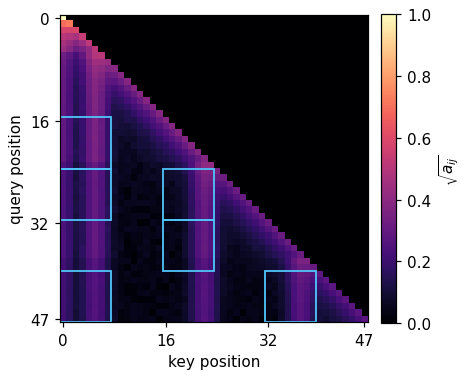
\includegraphics[width=0.8\linewidth]{figures/attention.png}
  \caption{Dense attention weights for one head of layer 18 on a 4k-token
  excerpt. Blocks selected by \textsc{Sieve} are outlined.}
  \label{fig:attention}
\end{figure}

\subsection{Ablations}

Removing the spread term $\sigma_i$ from the block score costs 2.1 points on
needle retrieval, and disabling selection reuse across layers increases
latency by 18\% with no change in accuracy. See \autoref{sec:analysis} for
why the spread term matters.
